\chapter{Residual-based VMS methods}
\label{chap-Rb_VMS}
\section{Introduction}
\label{sec-C4_introduction}

LES techniques for the numerical simulation of turbulent flows \cite{Sagaut2006} are based on a scale separation that permits to reduce the computational cost with respect to direct numerical simulation (DNS). Such scale separation is traditionally achieved by filtering the original Navier-Stokes equations, which leads to an extra forcing term defined by a physical (functional or structural) model. This widely used approach is usually referred to as explicit LES \cite{Sagaut2006}.

By contrast, implicit LES techniques (ILES) rely on purely numerical artifacts without any modification of the continuous problem. This approach was seldom followed, the MILES (Monotone Integrated LES) approach \cite{boris_new_1992,Fureby2002,Grinstein2007} being the main exception, until the VMS method was introduced \cite{hughes_multiscale_1995,hughes_variational_1998} and subsequently proposed as an ILES method (see below). ILES techniques are usually considered to be based on the addition of purely dissipative numerical terms, see  \cite[Section 5.3.4]{Sagaut2006}. It is worth to emphasize that this is not the case of some particular VMS models, as it is shown in \cite{principe_dissipative_2010} and discussed below.

VMS was introduced in \cite{hughes_multiscale_1995,hughes_variational_1998} as a framework for the motivation and development of stabilization techniques, which aim to overcome numerical difficulties encountered when using the standard Galerkin method. On the one hand, the velocity and pressure finite element (FE) spaces need to satisfy the \textit{inf-sup} compatibility condition that guarantees pressure stability and precludes the use of equal order interpolation. Mixed methods satisfying this condition can be used and their finite volume counterpart, based on staggered grids, are common in the LES community. Stabilization techniques that permit the use of equal order interpolation were proposed, e.g., in \cite{douglas_absolutely_1989,hughes_new_1986}. % , and finally recast into the VMS framework. 
On the other hand, global nonphysical oscillations appear in the convection dominated regime, when the mesh is not fine enough, that is, for high mesh Reynolds number flows. The only way to overcome this problem is through the addition of some form of dissipation which was recognized in the early development of stabilized methods \cite{brooks_streamline_1982}. Let us note that  the common practice in the LES community is to rely on the explicit extra term introduced by the physical model using high order approximations of the convective term.
\footnote{It is worth to point out that both problems (convection instability and compatibility conditions) are also present in the \textit{linear} Oseen problem. One of the inconsistencies of an explicit LES approach without a numerical dissipation term is that convection is stabilized by a term that comes from the physical model of the nonlinear Navier Stokes equations and such a term is not present when the linear Oseen problem is considered.} 

The first attempts to perform LES using VMS concepts, presented in \cite{hughes_large_2000,hughes_large_2001,hughes_multiscale_2001,koobus_variational_2004,john_variants_2008},  were performed introducing explicit subgrid modeling. The VMS models used in these works split resolved scales into large and small, introducing an explicit LES model to account for the small scales stress tensor, e.g., a Smagorinsky-type dissipative term acting on the small scales only. As a result, an important fraction of the degrees of freedom are used for the small resolved scales whereas consistency is retained in the large resolved scales only. 

ILES using a VMS approach with resolved and unresolved subgrid scales (the setting that permits to recover stabilized formulations) was suggested in \cite{codina_stabilized_2002} and performed in \cite{Calo_2004,bazilevs_variational_2007,nogueira_implicit_2010}. Excellent results were first presented in \cite{bazilevs_variational_2007}, but using isogeometric analysis for the space approximation \cite{Hughes_2005a}. Compared to classical LES based on filtering, the VMS approach does not face difficulties associated to inhomogeneous non-commutative filters in wall-bounded flows. Further, it retains numerical consistency in the FE equations and optimal convergence up to the interpolation order whereas, e.g., Smagorinsky models introduce a consistency error of order $h^{4/3}$ (see \cite{hughes_large_2000,hughes_large_2001,bazilevs_variational_2007}).

Scale separation is achieved in the VMS formalism by a variational projection. The continuous unknown is split into a resolvable FE component and an unresolvable subgrid or subscale component. The action of the subscales onto the FE scales can be approximated in different ways, leading to different VMS models but in all cases these models are {\em residual based} (no eddy viscosity is introduced), which permits to retain consistency. Among the modeling possibilities is the choice of the subscale space, first discussed in \cite{codina_stabilization_2000}, where it was enforced to be $L^2$-orthogonal to the FE space. Another modeling ingredient is the possibility of considering time-dependent subscales and to keep the VMS decomposition in all the nonlinear terms, which was studied in \cite{codina_stabilized_2002,codina_time_2007}. Clear improvements have been observed when using dynamic and fully nonlinear models for the simulation of laminar flows \cite{codina_time_2007, Avila2011}.

%Usually, the unresolved scales in LES methods are modeled by physical based models, see ... But it has been seen that variational multiscale methods (VMS) can reproduce the effect of the small scales in the flow, as it was introduced in Hughes et al. \cite{hughes_large_2001}. Bazilevs et al. in \cite{bazilevs_variational_2007} stress the fact that with this method additional models as eddy viscosities are not needed. 
%The Galerkin FE method used to solve the Navier-Stokes equations for incompressible flows it is known to have some numerical difficulties. For convection dominating problems, which is the case of high Reynolds number flows, the solution using the FE method has numerical inestabilities. There also are compatibility conditions between the velocity and pressure FE spaces that is the \textit{inf-sup} or \textit{LBB} condition. 
%To avoid this numerical drawbacks we use residual-based stabilized FE methods derived from the VMS concept. 

%The VMS method was introduced by Hughes \cite{hughes_multiscale_1995} and basically consists on a separition of scales by a variational projection. The coarse scale is resolved using the FE method while the small scale is modeled and introduced to the coarse scale equations without the need to add any subgrid viscosity. Later, Codina \cite{codina_stabilization_2000,codina_stabilized_2002} introduced the concept of orthogonal subscales where the subscale space is suposed to be orthogonal to the FE space. The time-dependence of the subscales was studied in \cite{codina_time_2007} and it is shown to exhibit better properties in terms of stability and accuracy.

In this chapter we assess implicit VMS models for the numerical simulation of turbulent flows. We refer to the original references for a comprehensive treatment of the assumptions of the formulations and their numerical analysis. Our intention here is to compare the different VMS schemes in terms of quality of the results and computational cost, and discuss some implementation aspects that we find particularly relevant for the simulation of turbulent flows. Our main motivation is to compare the influence of using orthogonal subscales, in order to enrich current comparisons on VMS techniques for large-eddy simulations, such as \cite{gamnitzer_time-dependent_2010}, where only non-projected subscales are considered. We present a detailed numerical experimentation for three well known problems: the decay of homogeneous isotropic turbulence (DHIT), the Taylor-Green vortex (TGV) and the turbulent flow in a channel (TCF), described in Section \ref{chap-Turbulence}. Thus, both unbounded and wall-bounded flows are considered; only wall-bounded tests are performed in \cite{gamnitzer_time-dependent_2010}. Some other differences with respect to \cite{gamnitzer_time-dependent_2010} are: 1) we consider a nonlinear sub-scale equation; 2) we do not include the time step size in the stabilization term; 3) we have analyzed the effect of the skew-symmetric term. 
 
The first implementation aspect we discuss is the treatment of the convective term. As it is well-known, the numerical analysis \cite{badia_convergence_2014,burman_galerkin_2009,guermond_faedogalerkin_2007} requires a skew-symmetric form of this term in order to avoid any positive contribution to the energy estimates that cannot be properly controlled. The construction of numerical schemes that preserve the skew-symmetry of the convective term at the discrete level has been long studied in the finite difference and finite volume contexts \cite{arakawa_computational_1966, verstappen_symmetry-preserving_2003, gassner_skew-symmetric_2013, trias_symmetry-preserving_2014, del_rey_fernandez_review_2014, svard_review_2014}. However, FE formulations used to perform VMS-based LES use either the conservative form \cite{hughes_large_2000,koobus_variational_2004,bazilevs_variational_2007,calderer_residual-based_2013, Calo_2004,gamnitzer_time-dependent_2010,gravemeier_algebraic_2010,masud_variational_2011} or the non-conservative one \cite{john_variants_2008,codina_time_2007,principe_dissipative_2010}. The approach we follow here is similar to that in \cite{Temam_1984} and is based on a split of the convective term into conservative and non-conservative terms. In the FE (variational) context, this simple approach guarantees the preservation of skew-symmetry at the discrete level. We remark that in the nonlinear VMS models the convective velocity is discontinuous (due to the subscale contribution), which prevents us to use some popular skewsymmetric forms. We also show numerically that a positive energy contribution actually appears if a non skew-symmetric form is used. 

The second point that we address is the use of weighted (by the stabilization parameter) projections and consistent mass matrices when orthogonal subscales are considered. Even though it is cheaper to use non-weighted projections and lumped mass matrices, only the use of consistent projections guarantees exact $L^2$ orthogonality. An alternative is the use of Scott-Zhang projections recently proposed in \cite{badia_stabilized_2012}, although we do not consider this approach here.

We also discuss the influence of the algorithmic constants of the stabilization parameters in the numerical results. In particular, we show that the choice of the stabilization parameter multiplying the div-div term has a strong influence on the numerical results while it is not essential for stability and convergence of the methods. We further analyze the behavior of the VMS formulation as the time step size is reduced. These two facts are actually related by the way the stabilization parameters are usually defined (see \cite{gamnitzer_time-dependent_2010,hsu_improving_2010}).

Finally, we compare the results obtained using VMS models against those obtained using classical LES based on filtering and the dynamic Smagorinsky closure \cite{fauconnier_construction_2009}, and another implicit LES method, the adaptive local deconvolution presented in \cite{hickel_adaptive_2006}. 
%We do so comparing against other author results for the TGV test, using dynamic Smagorinsky and adaptive local deconvolution methods \cite{fauconnier_construction_2009,hickel_adaptive_2006}.
%We do so using the Galerkin approximation of the Navier Stokes equations with a Taylor-Hood $Q$2/$Q$1 interpolation which satisfies the inf-sup condition, relying on the Smagorinsky term to stabilize convection as it is usually done in the LES community. 

The chapter is organized as follows. In Section \ref{sec-C4_prob_statement} we present the VMS formulation, how to compute truly orthogonal subscales and the different models we aim at analyzing, whereas in Section \ref{sec-C4_energy} we discuss energy conservation statements and how they are influenced by the choice of the VMS method and the definition of the convective term. Sections \ref{subsec-C4_DHIT},  \ref{subsec-C4_TGV},  \ref{subsec-C4_TCF} are devoted to the numerical approximation of the DHIT, the TGV, and the TCF problems, respectively. Sections \ref{subsec-C4_effect_const} and \ref{subsec-C4_small_time_step} discuss the effect of the algorithmic constants on the results and the behavior of the different schemes in the small time step limit. Some remarks close the article in Section \ref{sec-C4_conclusions}.

%We will not restrict our atention only in the physical point of view, but we also are interested in the numerical conclusions. For instance, we will evaluate the computational cost of the different methods. Another interesting analysis that has been carried out in this article is the stability for the small time-step limit. Gammitzer et al. \cite{gamnitzer_time-dependent_2010} studied the influence of introducing the dependency of the stabiliztion parameters on the time step, proposed by Bazilevs et al. \cite{bazilevs_variational_2007}, in order to avoid convergence problems at small time-steps.

%Other remarks will be made in the present paper concerning on the importance of a correct formulation of the VMS methods. That will include some analysis on the definition of the nonlinear convective term, the nonlinearity of the advection velocity, the correct definition of the projection when using orthogonal subscales or the importance of the algorithmic constants in the stabilization parameters.

\section{Problem statement}
\label{sec-C4_prob_statement}
\subsection{The Galerkin semi-discrete problem}
%\subsection{Navier-Stokes problem}
\label{subsec-C4_NS_formulation}
In order to improve the readability of this chapter we refresh the Navier-Stokes formulation that was already stated in \Chap{Preliminaries}. 

Let $\Omega$ be a bounded domain of $\mathbb{R}^d$, where $d=2,3$ is the number of space dimensions, $\Gamma=\partial\Omega$ its boundary and $[0,T]$ the time interval. The strong form of the incompressible Navier-Stokes problem consists of finding the velocity field $\u$ and the pressure field $p$ such that 
\begin{align}
\label{eq-C4_NS_strong_mome}
\partial_t\u-\nu\Delta\u+\u\cdot\nabla\u+\nabla p&=\f&\mbox{in $\Omega\times(0,T)$,}\\
\label{eq-C4_NS_strong_inc}
\nabla\cdot\u&=0&\mbox{in $\Omega\times(0,T)$,}
\end{align}
with $\f$ the force vector and $\nu$ the kinematic viscosity. 

Equations (\ref{eq-C4_NS_strong_mome})-(\ref{eq-C4_NS_strong_inc}) have to be supplied with appropriate boundary and initial conditions. The boundary $\Gamma$ is divided into the Dirichlet ($\Gamma_D$) and the Neumann ($\Gamma_N$) parts such that $\Gamma_D\cup\Gamma_N=\Gamma$ and $\Gamma_D\cap\Gamma_N=\emptyset$. Then, the boundary and initial conditions can be written as
\begin{align}
\label{eq-C4_NS_strong_Dir}
\u&=\u_g&\mbox{on $\Gamma_D\times(0,T]$,}\\
\label{eq-C4_NS_strong_Neu}
(-p \mathbf{I}+\nu(\nabla\u+\nabla\u^T))\cdot\mathbf{n}&=\mathbf{t}_N&\mbox{on $\Gamma_N\times(0,T]$,}\\
\label{eq-C4_NS_strong_Ini}
\u(\x,0)&=\u_0(\x)&\mbox{in $\Omega\times\{0\}$,}
\end{align}
$\mathbf{n}$ being the unit outward vector normal to $\Gamma$. To simplify the exposition, we will consider $\u_g = {\bf 0}$ and $\Gamma_D = \Gamma$ in what follows.

The weak form of the incompressible Navier-Stokes problem (\ref{eq-C4_NS_strong_mome})-(\ref{eq-C4_NS_strong_Ini}) consists, e.g., in finding $[\u,p]\in {L}^2(0,T;\mathcal{V}_0)\times {\cal D}'(0,T;\mathcal{Q}_0)$ (distributions in time with values in $\mathcal{Q}_0$) such that
\begin{equation}
\label{eq-C4_NS_weak}
(\partial_t\u,\v) + B(\u;[\u,p],[\v,q]) = \left<\f,\v\right> 
\quad\quad\forall\v\in\mathcal{V}_0,\quad\forall q\in\mathcal{Q}_0,
\end{equation}
satisfying the initial condition (\ref{eq-C4_NS_strong_Ini}) in a weak sense. Here $\mathcal{V}_0:={H}_0^1(\Omega)^d$, $\mathcal{Q}_0:=L^2(\Omega)/\mathbb{R}$ and the form $B({\a};[\u,p],(\v,q))$ is defined as 
\begin{equation}
\label{eq-C4_bilinear}
B(\a;[\u,p],[\v,q]):=\nu(\nabla\u,\nabla\v)+b(\a,\u,\v)-(p,\nabla\cdot\v)+(q,\nabla\cdot\u)
\end{equation}
where the trilinear weak form of the convective term $b(\u,\v,\w)$ can be written in the following three equivalent ways
\begin{align}
\label{eq-C4_b_noskew}
&b(\u,\v,\w)=(\u\cdot\nabla\v,\w)&&\mbox{Non conservative},\\
\label{eq-C4_b_skew1}
&b(\u,\v,\mathbf{w})=\frac{1}{2}(\u\cdot\nabla\v,\mathbf{w})-\frac{1}{2}(\v,\u\cdot\nabla\mathbf{w})&&\mbox{Skew-symmetric (type 1)},\\
\label{eq-C4_b_skew2}
&b(\u,\v,\mathbf{w})=(\u\cdot\nabla\v,\mathbf{w})+\frac{1}{2}(\v\cdot\mathbf{w},\nabla\cdot\u)&&\mbox{Skew-symmetric (type 2)}.
\end{align}
This equivalence is lost at the discrete level. The skew-symmetric form (type 2) (\ref{eq-C4_b_skew2}) is very common when numerical analysis are presented \cite{badia_convergence_2014,burman_galerkin_2009,guermond_faedogalerkin_2007} but the skew-symmetric form (type 2) (\ref{eq-C4_b_skew1}) has important advantages when the first argument is a discontinuous function, as will be shown below.

Let us now consider a FE partition $\mathcal{T}_h$ of the domain $\Omega$ from which we can construct conforming finite dimensional spaces for the velocity $\mathcal{V}_{0,h} \subset \mathcal{V}_0$, and for the pressure $\mathcal{Q}_{0,h}\subset \mathcal{Q}_0$. 

The Galerkin FE approximation of (\ref{eq-C4_NS_weak}) consists in finding $[\u_h,p_h]\in {L}^2(0,T;\mathcal{V}_{0,h})\times {\cal D}'(0,T;\mathcal{Q}_{0,h})$ such that
\begin{equation}
\label{eq-C4_NS_galerkin}
(\partial_t\u_h,\v_h) + B(\u_h;[\u_h,p_h],[\v_h,q_h]) =\left<\f,\v_h\right>
\quad\quad\forall\v_h\in\mathcal{V}_{0,h},\forall q_h\in\mathcal{Q}_{0,h}.
\end{equation}

\subsection{VMS framework}
\label{subsec-C4_VMS_framework}
As it was pointed out in \Sec{C2_vms}, the Galerkin FE formulation \Eq{C4_NS_galerkin} suffers from numerical instabilities for high mesh Reynolds number problems, i.e., convection dominated flows. The discrete \textit{inf-sup} condition that must be satisfied by the pair $\mathcal{V}_{0,h} \times\mathcal{Q}_{0,h}$ in order to have a well-posed problem with bounded pressure is also a problem that arise in the Galerkin FE formulation. The VMS method described in \Sec{C2_vms} overcomes these two instabilities.

After the space splitting into the FE space and the subscale space $\mathcal{V}_0=\mathcal{V}_{0,h}\oplus\widetilde{\mathcal{V}}_0$ and $\mathcal{Q}=\mathcal{Q}_{0,h}\oplus\widetilde{\mathcal{Q}}_0$, where $\widetilde{\mathcal{V}}_0$ and $\widetilde{\mathcal{Q}}_0$ are infinite-dimensional spaces that complete the FE spaces in $\mathcal{V}_0$ and $\mathcal{Q}_0$, respectively. The VMS semi-discrete problem reads: find $[\u_h,p_h]\in {L}^2(0,T;\mathcal{V}_{0,h})\times {\cal D}'(0,T;\mathcal{Q}_{0,h})$ such that
\begin{equation}
\label{eq-C4_NS_discrete}
(\partial_t\u_h,\v_h)+(\partial_t\tilde{\u},\v_h)+B(\a;[\u_h,p_h],[\v_h,q_h])+\left(\tilde{\u},\mathcal{L}_{\a}^*(\v_h,q_h)\right)_h-\left(\tilde{p},\nabla\cdot\v_h\right)=\left<\f,\v_h\right>.
\end{equation}
Where $ \mathcal{L}_{\a}^*(\v_h,q_h) $ is the adjoint operator defined in \Eq{C2_adjoint}. The fine scale problem is approximated by
\begin{align}
\label{eq-C4_velo_sgs}
\partial_t\tilde{\u}+\tau_m^{-1}\tilde{\u}=\mathcal{P}(\R_u),\\
\label{eq-C4_press_sgs}
\tau_c^{-1}\tilde{p}=\mathcal{P}(R_p).
\end{align}
With $ \R_u $ the momentum equation residual \Eq{C2_Ru}, $ R_p $ the continuity equation residual \Eq{C2_Rp}. $ \tau_m $ and $ \tau_c $ are the momentum and continuity equations stabilization parameters, respectively, which definition is given by 
\begin{align}
\label{eq-C4_tau_m}
&\tau_m=\left(\frac{c_1\nu}{h^2}+\frac{c_2|\a|}{h}\right)^{-1},\\
\label{eq-C4_tau_c}
&\tau_c=\frac{h^2}{c_1\tau_m}.
\end{align}

The particular VMS method will result from the combination of the three particular ingredients discussed in Sections \ref{subsec-C2_dyn}-\ref{subsec-C2_oss}, the dynamics of the subscale velocity, the nonlinearity of the advection velocity and the definition of the projection.

\section{Energy balance statements}
\label{sec-C4_energy}

In this section we revisit global energy conservation statements of the method. As shown in \cite{principe_dissipative_2010}, similar statements can be obtained locally (in a volume $\omega \subset \Omega$).

Taking $\v_h=\u_h$ and $q_h=p_h$ in (\ref{eq-C4_NS_discrete}) we have the energy balance on the FE component
\begin{align}
\label{eq-C4_FE_balance2}
\underbrace{\frac{1}{2}d_t\|\u_h\|^2}_I
& +\underbrace{\nu\|\nabla\u_h\|^2}_{II}
  +\underbrace{b(\a,\u_h,\u_h)}_{III} \\ \nonumber
& +\underbrace{(\partial_t\tilde{\u},\u_h)
+\left(\tilde{\u},\mathcal{L}^*_{\a}(\u_h,p_h)\right)_h
-\left(\tilde{p},\nabla\cdot\u_h\right)}_{IV}
=\underbrace{\left<\mathbf{f},\mathbf{u}_h\right>}_V,
\end{align}
In equation (\ref{eq-C4_FE_balance2}) we group the terms as
% \begin{center}
% \begin{tabular}{rll}
% I)&FE time derivative term:&$\frac{1}{2}d_t\|\u_h\|^2$\\
% II)&FE viscous term:&$\nu\|\nabla\u_h\|^2$\\
% III)&Convective term:&$b(\a,\u_h,\u_h)$\\
% IV)&FE to subscale energy transfer terms:&$(\partial_t\tilde{\u},\u_h)-\left(\tilde{\u},\mathcal{L}^*_{\a}(\u_h,p_h)\right)-\left(\tilde{p},\nabla\cdot\u_h\right)$\\
% V)&FE work of external power:& $\left<\mathbf{f},\mathbf{u}_h\right>$\\
% \end{tabular}
% \end{center}
\begin{center}
\begin{tabular}{rll}
I)&FE kinetic energy variation:&$\frac{1}{2}d_t\|\u_h\|^2$\\
II)&FE viscous dissipation:&$\nu\|\nabla\u_h\|^2$\\
III)&FE convective term:&$b(\a,\u_h,\u_h)$\\
IV)&FE to SGS energy transfer:&$\varepsilon_{h} =(\partial_t\tilde{\u},\u_h)+\left(\tilde{\u},\mathcal{L}^*_{\a}(\u_h,p_h)\right)_h-\left(\tilde{p},\nabla\cdot\u_h\right)$\\
V)&FE component of external power:& $\left<\mathbf{f},\mathbf{u}_h\right>$\\
\end{tabular}
\end{center}
Multiplying (\ref{eq-C4_velo_sgs}) by $\tilde{\u}$ and (\ref{eq-C4_press_sgs}) by $\tilde{p}$, integrating over the domain and decomposing the residual of the momentum equation as $\R_u=\f-\partial_t\u_h-\mathcal{L}_{\a}(\u_h,p_h)$, % we have from (\ref{eq-C4_sgs_balance1}) 
we obtain the global energy balance on the fine scale
\begin{align}
\label{eq-C4_sgs_balance2}
\underbrace{\frac{1}{2}d_t\|\tilde{\u}\|^2}_I
&+\underbrace{\tau_m^{-1}\|\tilde{\u}\|^2}_{II}
+\underbrace{\tau_c^{-1}\|\tilde{p}\|^2}_{III} \\ \nonumber
&+\underbrace{\left(\mathcal{P}(\partial_t\u_h),\tilde{\u}\right)
+\left(\mathcal{P}(\mathcal{L}_{\a}(\u_h,p_h)),\tilde{\u}\right)_h
+\left(\mathcal{P}(\nabla\cdot\u_h),\tilde{p}\right)}_{IV}
=\underbrace{\left(\mathcal{P}(\f),\tilde{\u}\right)}_V.
\end{align}
% In equation (\ref{eq-C4_sgs_balance2}) we group the terms as
% \begin{center}
% \begin{tabular}{rll}
% I)&Subscale time derivative term:&$\frac{1}{2}d_t\|\tilde{\u}\|^2$\\
% II)&Subscale viscous term:&$\tau_m^{-1}\|\tilde{\u}\|^2$\\
% III)&Subscale pressure term:&$\tau_c^{-1}\|\tilde{p}\|^2$\\
% IV)&Subscale to FE energy transfer balance:&$\left(\mathcal{P}(\partial_t\u_h),\tilde{\u}\right)+\left(\tilde{\u},\mathcal{P}(\mathcal{L}_{\a}(\u_h,p_h))\right)+\left(\tilde{p},\mathcal{P}(\nabla\cdot\u_h)\right)$\\
% V)&Subscale work of external power:&$\left(\mathcal{P}(\f),\tilde{\u}\right)$\\
% \end{tabular}
% \end{center}
We group the terms in (\ref{eq-C4_sgs_balance2}) as
\begin{center}
\begin{tabular}{rll}
I)&SGS kinetic energy variation:&$\frac{1}{2}d_t\|\tilde{\u}\|^2$\\
II)&SGS velocity dissipation:&$\tau_m^{-1}\|\tilde{\u}\|^2$\\
III)&SGS pressure dissipation:&$\tau_c^{-1}\|\tilde{p}\|^2$\\
IV)&SGS to FE energy transfer:&$\tilde{\varepsilon}= \left(\mathcal{P}(\partial_t\u_h),\tilde{\u}\right)+\left(\tilde{\u},\mathcal{P}(\mathcal{L}_{\a}(\u_h,p_h))\right)_h+\left(\tilde{p},\mathcal{P}(\nabla\cdot\u_h)\right)$\\
V)&SGS component of external power:&$\left(\mathcal{P}(\f),\tilde{\u}\right)$\\
\end{tabular}
\end{center}
Finally, adding up equations (\ref{eq-C4_FE_balance2}) and (\ref{eq-C4_sgs_balance2}) 
%and using $\mathcal{L}^*(\u_h,p_h)=-\mathcal{L}(\u_h,p_h)$ for linear elements, 
we obtain an equation for the total kinetic energy
\begin{align}
\label{eq-C4_total_balance}
   \frac{1}{2}d_t\|\u_h\|^2
& +\frac{1}{2}d_t\|\tilde{\u}\|^2
  +\nu\|\nabla\u_h\|^2+b(\a,\u_h,\u_h)
  +\tau_m^{-1}\|\tilde{\u}\|^2+\tau_c^{-1}\|\tilde{p}\|^2 \\ \nonumber
& +(\partial_t\tilde{\u},\u_h)
  +\left(\mathcal{P}(\partial_t\u_h),\tilde{\u}\right)
  +\left(\mathcal{P}(\mathcal{L}_{\a}(\u_h,p_h))+\mathcal{L}^*_{\a}(\u_h,p_h),\tilde{\u}\right)_h\\ \nonumber
& \quad \quad \quad \quad  +\left(\mathcal{P}(\nabla\cdot\u_h)-\nabla\cdot\u_h,\tilde{p}\right)=\left<\mathbf{f},\mathbf{u}_h\right>+\left((\mathcal{P}(\f),\tilde{\u}\right).
\end{align}
%Even though it is not our intention to perform a numerical analysis of the methods, let us review known results for each particular VMS model. 
Let us note the presence of $b(\a,\u_h,\u_h)$, which is zero only when the skew-symmetric type 1 form is considered. Other choices could result in a spurious positive contribution to the FE kinetic energy as it is actually observed in the DHIT problem, and could result in a loss of stability, although that was not observed.
%We restric the discussion to the linear version of the multiscale splitting, we are not aware of any result about the fully nonlinear case.

\subsection{Static subscales} 

In this case the energy balance for the subscale is meaningless because there are explicit expressions for the subscales (\ref{eq-C2_static_sgs}) and (\ref{eq-C4_press_sgs}). When (\ref{eq-C2_static_sgs}) and (\ref{eq-C4_press_sgs}) are used in (\ref{eq-C4_FE_balance2}), we obtain
\begin{align}
\label{eq-C4_static_energy}
\frac{1}{2}d_t\|\u_h\|^2
& +\nu\|\nabla\u_h\|^2 + b(\a,\u_h,\u_h)  
  + \left( \tau_{m} \mathcal{P} \left(  \partial_t \u_h \right), \mathcal{L}^*_{\a} ( \u_{h},p_h)\right)_h \\ \nonumber
& + \left(\tau_{m} \mathcal{P} \left( \mathcal{L}_{\a} ( \u_{h},p_h) \right),\mathcal{L}^*_{\a}(\u_h,p_h)\right)_h
%+ \left(\tau_{c} \mathcal{P} (\nabla \cdot \u_{h}),\nabla\cdot\u_h\right)
+ \tau_{c} \left\| \mathcal{P}(\nabla \cdot \u_{h})\right\|^{2}\\ \nonumber
& = \langle\mathbf{f},\mathbf{u}_h\rangle + \left(\tau_m \mathcal{P}(\mathbf{f}),\mathcal{L}^*_{\a}(\u_h,p_h)\right)_h.
\end{align}
In the case of the ASGS method, where $\mathcal{P}:=\mathbf{I}$, the fourth term on the left hand side is a source of problems. One the one hand, it cannot be neglected because it is needed to make the method consistent. On the other hand, it can only be controlled by the dissipation of the time integration scheme and is therefore responsible for the introduction of a restriction on the time step size. As a side problem, it is very inconvenient for an implementation if any explicit (operator splitting) time integration is chosen as it results in a non-symmetric mass matrix. This term is not present if the OSS method is chosen using the projection $\mathcal{P}:=\mathbf{I}-\Pi_h$. Stability of both the fully discrete and the semidiscrete Stokes problem have been proven in \cite{badia_multiscale_2009}.

The important term is the fifth one, which permits to control
$ \tau_{m} \left\| \mathcal{P} \left( \mathbf{a}\cdot \mathbf{\nabla u}_{h}+\mathbf{\nabla }p_{h}\right) \right\|^{2} $; the FE part in the OSS formulation is readily controlled using inverse estimates. It therefore provides the essential numerical stability. The last term acts as a penalty on the divergence constraint, adding volumetric diffusion and provides (extra, non-essential) numerical stability.

For the OSS method, it is proved in \cite{guasch_statistical_2013} that the dissipative structure of the discrete problem has the same statistical behavior in fully developed turbulence than the continuous problem, in the sense that this dissipation has the same estimates as the molecular one. Both dissipations could be made equal by a proper choice of the stabilization parameters in (\ref{eq-C4_tau_m}). This, however, requires a small change in the advection velocity of this expression, which depends on an integral length of the problem. See \cite{guasch_statistical_2013} for details.

\subsection{Dynamic subscales} 

In this case, the time derivative of both the FE and subgrid components have to be considered and an estimator for the kinetic energy variation of both the FE and subgrid velocity can be obtained. The stability of the subgrid scale velocity can then be used to obtain a stability estimate of the FE component in a norm that includes the convective and pressure terms \cite{codina_time_2007,badia_multiscale_2009,Badia2010}.\footnote{However, it should be kept in mind that the numerical solution of the problem is the FE component. There is no reason to add the subscale to the final solution as the approximation is limited by the interpolation order, see \cite[Remark 10]{codina_time_2007}.} Therefore, the numerical dissipation of the method is actually given by the energy transfer $\varepsilon_h$ from the FE to the subscale component. 
Using (\ref{eq-C4_velo_sgs})-(\ref{eq-C4_press_sgs}), we get:
\begin{align}
\label{eq-C4_transfer}
\varepsilon_{h} & = 
  \left( \partial_t\tilde{\u} , \u_h\right) 
- \left( \tau_m \partial_t\tilde{\u} , \mathcal{L}^*_{\a} ( \u_{h},p_h)\right) _h 
- \left( \tau_{m} \mathcal{P} \left(  \partial_t \u_h \right), \mathcal{L}^*_{\a} ( \u_{h},p_h)\right)_h \\ \nonumber
& 
- \left( \tau_{m} \mathcal{P} \left(  \mathcal{L}_{\a} ( \u_{h},p_h) \right), \mathcal{L}^*_{\a} ( \u_{h},p_h) \right)_h
+ \tau_{c} \left\| \mathcal{P} \nabla \cdot \u_{h}\right\|^{2}. %\nonumber
\end{align}
Except from the viscous contribution, the last two terms in (\ref{eq-C4_transfer}) are positive, providing dissipation of the FE energy, but the first three could be negative, providing these models with a mechanism to predict a backward energy transfer, not frequently found in classical LES models \cite{Sagaut2006}. It is justified in \cite{Codina-chap-2011} that even if the first three terms may be negative at a certain time instant, their averaged contribution in a time window greater than the largest period needs to be positive, which is the behavior expected of backscatter from a physical point of view. 

For the ASGS method, i.e., $\mathcal{P}:=\mathbf{I}$, the last term in the left hand side of (\ref{eq-C4_total_balance}) vanishes and the previous one reads
\begin{equation}
\left(\mathcal{L}_{\a}(\u_h,p_h)+\mathcal{L}^*_{\a}(\u_h,p_h),\tilde{\u}\right)_h=
-2 \left(\nu\Delta\u_h,\tilde{\u}\right)_h.
\end{equation}
In turn, the time derivatives of the FE and subscale velocities can be combined as
\begin{align}
\label{eq-C4_time_deriv_ASGS}
\frac{1}{2}d_t\|\u_h\|^2+\frac{1}{2}d_t\|\tilde{\u}\|^2+(\partial_t\tilde{\u},\u_h)+\left(\partial_t\u_h,\tilde{\u}\right)=\frac{1}{2}d_t\|\u_h+\tilde{\u}\|^2
\end{align}
to rewrite (\ref{eq-C4_total_balance}) as
\begin{align}
\label{eq-C4_total_balance_ASGS2}
\frac{1}{2}d_t\|\u_h+\tilde{\u}\|^2
&+\nu\|\nabla\u_h\|^2+b(\a,\u_h,\u_h) \\ \nonumber
&+\tau_m^{-1}\|\tilde{\u}\|^2+\tau_c^{-1}\|\tilde{p}\|^2-2 \left(\nu\Delta\u_h,\tilde{\u}\right)=\left<\mathbf{f},\mathbf{u}_h\right>+\left<\mathbf{f},\tilde{\u}\right>.
\end{align}
From this equation, a stability estimate for $\|\u_h+\tilde{\u}\|$ can be obtained as the last term on the left hand side can be controlled using the second one (see \cite[Remark 4.7]{badia_multiscale_2009}).% where this stability is proven for the Stokes problem.

Another important point of (\ref{eq-C4_total_balance_ASGS2}) is that it immediately shows that when the mesh is fine enough, i.e., 
\begin{equation*}
\frac{\left| \mathbf{a}\right| h}{\nu }\ll 1,
\end{equation*}
the dissipation of the total energy depends only on the viscosity. Therefore, the dissipative structure is correctly predicted when a laminar flow is considered or when the discretization is fine enough to resolve all scales of the flow, an important advantage over other LES techniques.

On the other hand, for the OSS method, the FE and subgrid kinetic energy can be summed to obtain the total one
\begin{align}
\label{eq-C4_time_deriv_OSS}
\frac{1}{2}d_t\|\u_h\|^2+\frac{1}{2}d_t\|\tilde{\u}\|^2=\frac{1}{2}d_t\|\u_h+\tilde{\u}\|^2.
\end{align}
since $(\partial_t\tilde{\u},\u_h)=(\partial_t\u_h,\tilde{\u})=0$ as soon as we enforce the subscale to be orthogonal to the FE space. This property also guarantees that%{\color{red} (OJO!! si $\mathcal{P}\left(\partial_t\tilde{\u}\right)+\tau_m^{-1}\tilde{\u}=\mathcal{P}(\R_u)$ esto no se cumple con $\mathcal{P}\equiv\Pi^\bot$ porque $(\mathcal{P}(\partial_t\tilde{\u}),\u_h)=0\Rightarrow(\partial_t\tilde{\u},\u_h)=(\Pi_\tau(\partial_t\tilde{\u}),\u_h)\neq0$. Es asi??)} 
\begin{align}
\label{eq-C4_Pi_tau_sgs}
\left(\Pi_m(\mathcal{L}_{\a}(\u_h,p_h)),\tilde{\u}\right) = 0 \\
\left(\Pi_c(\nabla\cdot\u_h),\tilde{p}\right)=0
\end{align}
which implies that the last term on the left hand side of (\ref{eq-C4_total_balance}) vanishes and that the previous one can be written as
\begin{align}
\left(\mathcal{P}(\mathcal{L}_{\a}(\u_h,p_h))+\mathcal{L}^*_{\a}(\u_h,p_h),\tilde{\u}\right)_h
= \left( (\mathcal{L}_{\a}(\u_h,p_h)+\mathcal{L}^*_{\a}(\u_h,p_h),\tilde{\u}\right)_h
=-2 \left(\nu\Delta\u_h,\tilde{\u}\right)_h
\end{align}
as in the ASGS case. Let us note that the Laplacian term can be eliminated without affecting the convergence properties of the method. 
%It can be justified by replacing the elementwise Laplacian by a discrete Laplacian operator in $\mathcal{L}_{\a}$ (see \cite{badia_implementation_2013}). 
% {\color{blue}Note that if the dynamic definition of the subscales is considered, the condition (\ref{eq-C4_Pi_tau_sgs}) is achieved only if we use the modified subscale equation (\ref{eq-C4_velo_sgs_projected}) instead of (\ref{eq-C4_velo_sgs}). Using the definition (\ref{eq-C4_Pi_tau_m}) we have that
% \begin{align}
% \label{eq-C4_Pi_tau_sgs_demo}
% \left(\Pi_m(\mathcal{L}_{\a}(\u_h,p_h)),\tilde{\u}\right) 
% & = \left(\Pi_m(\mathcal{L}_{\a}(\u_h,p_h)),\tau_m\mathcal{P}(\R_u)\right)\\\nonumber
% &  -\left(\Pi_m(\mathcal{L}_{\a}(\u_h,p_h)),\tau_m\mathcal{P}(\partial_t\tilde{\u})\right)\\\nonumber
% & = \left(\Pi_m(\mathcal{L}_{\a}(\u_h,p_h)),\tau_m\R_u\right) 
%   - \left(\Pi_m(\mathcal{L}_{\a}(\u_h,p_h)),\tau_m\Pi_m(\R_u)\right)\\\nonumber
% & - \left(\Pi_m(\mathcal{L}_{\a}(\u_h,p_h)),\tau_m\partial_t\tilde{\u}\right)
%   + \left(\Pi_m(\mathcal{L}_{\a}(\u_h,p_h)),\tau_m\Pi_m(\partial_t\tilde{\u})\right)\\\nonumber
% & = 0.
% \end{align}}
Then, the global energy balance equation (\ref{eq-C4_total_balance}) reads
\begin{align}
\label{eq-C4_total_balance_OSS2}
\frac{1}{2}d_t\|\u_h\|^2+\frac{1}{2}d_t\|\tilde{\u}\|^2
&+\nu\|\nabla\u_h\|^2+b(\a,\u_h,\u_h) \\ \nonumber
&+\tau_m^{-1}\|\tilde{\u}\|^2+\tau_c^{-1}\|\tilde{p}\|^2 %- 2 \left(\nu\Delta\u_h,\tilde{\u}\right)
=\left<\mathbf{f},\mathbf{u}_h\right>+\left(\mathcal{P}(\mathbf{f}),\tilde{\u}\right),
\end{align}
which is exactly (\ref{eq-C4_total_balance_ASGS2}) except for the projection of the force in the last term. Stability and convergence of this formulation have been proved in \cite{Badia2010,badia_convergence_2014}.

\section{Final discrete problem}
\label{sec-C4_discrete}
Applying a time integration algorithm to (\ref{eq-C4_NS_discrete})-(\ref{eq-C4_velo_sgs})-(\ref{eq-C4_press_sgs}) we get the fully discrete problem. The final implementation of the discrete problem is written here considering a Picard linearization of the convective term and the Backward Euler (BE) scheme for the time discretization. It can be straightforwardly modified to consider the Crank-Nicolson time integration scheme; this last scheme is the one used in the numerical examples of Sections \ref{subsec-C4_DHIT},  \ref{subsec-C4_TGV} and \ref{subsec-C4_TCF}.

Some tips and comments on the implementation of the methods described hereinafter are given in Appendix \ref{appendix-VMS_implementation}.

\subsection{Algebraic Subgrid Scales (ASGS)}

Taking the nonlinear advection velocity definition \Eq{C2_a_nl} and considering the time derivative in the fine scales, we have the Dynamic and Nonlinear ASGS method, hereinafter Dyn-Nl-ASGS. 
%For this method, using linear FEs, the Backward Euler (BE) scheme for the time discretization and the Picard method for the nonlinear term, 
At time step $n$ and nonlinear iteration $i$, given $\u_h^{n,i-1}$, $\u_h^{n-1}$, $\tilde{\u}^{n,i-1}$ and $\tilde{\u}^{n-1}$ we compute $\mathbf{u}_h^{n,i}$ and $ p_h^{n,i} $ such that
% \begin{align}
% \label{eq-C4_Dyn-Nl-ASGS}
% &\frac{1}{\Delta t}(\u_h^{n+1,i},\v_h)+\nu(\nabla\u_h^{n+1,i},\nabla\v_h)+b(\a^{n+1,i-1},\u_h^{n+1,i},\v_h)-(p_h^{n+1},\nabla\cdot\v_h)+(q_h,\nabla\cdot\u_h^{n+1,i})+\\\nonumber
% &+\left(\tau_{m,t}\left[\frac{1}{\Delta t}\u_h^{n+1,i}+N(\a^{n+1,i-1},\u_h^{n+1,i})+\nabla p_h^{n+1}\right],N(\a^{n+1,i-1},\v_h)+\nabla q_h\right)+\\\nonumber
% &+\left(\tau_c\nabla\cdot\u_h^{n+1,i},\nabla\cdot\v_h\right)-\frac{1}{\Delta t}\left(\tau_{m,t}\left[\frac{1}{\Delta t}\u_h^{n+1,i}+N(\a^{n+1,i-1},\u_h^{n+1,i})+\nabla p_h^{n+1}\right],\v_h\right)=\\\nonumber
% &=\langle\v_h,\mathbf{f}\rangle+\frac{1}{\Delta t}(\u_h^{n},\v_h)+\frac{1}{\Delta t}(\tilde{\u}^{n},\v_h)+\left(\tau_{m,t}\left[\frac{1}{\Delta t}\u_h^{n}+\mathbf{f}+\frac{1}{\Delta t}\tilde{\u}^n\right],N(\a^{n+1,i-1},\v_h)+\nabla q_h\right)-\\\nonumber
% &-\frac{1}{\Delta t}\left(\tau_{m,t}\left[\frac{1}{\Delta t}\u_h^{n}+\mathbf{f}+\frac{1}{\Delta t}\tilde{\u}^n\right],\v_h\right),\\\nonumber
% \end{align}
\begin{align}
\label{eq-C4_Dyn-Nl-ASGS}
\frac{1}{\delta t}(\u_h^{n,i},\v_h)
&+ B(\a^{n,i-1};[\u_h^{n,i},p_h^{n,i}],[\v_h,q_h])
\\ \nonumber
&+\left(\tau_{m,t} \left[\frac{1}{\delta t}\u_h^{n,i}+ \mathcal{L}_{\a^{n,i-1}}(\u_h^{n,i},p_h^{n,i})\right], \mathcal{L}^*_{\a^{n,i-1}}(\v_h,q_h) \right)_h\\ \nonumber
&+\left(\tau_c\nabla\cdot\u_h^{n,i},\nabla\cdot\v_h\right)
-\frac{1}{\delta t} \left(\tau_{m,t}\left[\frac{1}{\delta t}\u_h^{n,i}+ \mathcal{L}_{\a^{n,i-1}}(\u_h^{n,i},p_h^{n,i})\right],\v_h\right)_h \\\nonumber
&=\langle\v_h,\mathbf{f}\rangle
+\frac{1}{\delta t}(\u_h^{n-1},\v_h)+\frac{1}{\delta t}(\tilde{\u}^{n-1},\v_h) \\\nonumber
&-\frac{1}{\delta t}\left(\tau_{m,t}\left[\frac{1}{\delta t}\u_h^{n-1}+\mathbf{f}+\frac{1}{\delta t}\tilde{\u}^{n-1}\right],\v_h\right) \\\nonumber
&+\left(\tau_{m,t}\left[\frac{1}{\delta t}\u_h^{n-1}+\mathbf{f}+\frac{1}{\delta t}\tilde{\u}^{n-1}\right],\mathcal{L}^*_{\a^{n,i-1}}(\v_h,q_h) \right)_h,
\label{eq-C4_Dyn-Nl-ASGS}
\end{align}
where $\tau_{m,t}=\left(\delta t^{-1}+\tau_m^{-1}\right)^{-1}$ and $\a^{n,i-1}=\u_h^{n,i-1}+\tilde{\u}^{n,i-1}$.

In turn, $\tilde{\u}^{n,i}$ is computed by solving the discretization of the fine scale problem (\ref{eq-C4_velo_sgs}). Note that in the nonlinear version of the algorithm, the stabilization parameter $\tau_{m,t}$ depends on the subscale itself through $\a$ in (\ref{eq-C4_tau_m}), making the fine scale equation also nonlinear, although it is local and does not increase the size of the global linear system to be solved. At each integration point of each element we iteratively solve
\begin{equation}
\label{eq-C4_velo_sgs_discrete_expl}
\tilde{\mathbf{u}}^{n,i,k}=\tau_{m,t}^{k-1}\frac{1}{\delta t}\tilde{\mathbf{u}}^{n-1}
+ \tau_{m,t}^{k-1} \left[\mathbf{f} - \frac{(\u_h^{n,i}-\u_h^{n-1})}{\delta t} - \mathcal{L}_{\a^{n,i,k-1}}(\u_h^{n,i},p_h^{n,i})\right].
%\left(\frac{(\u_h^{n+1,i}-\u_h^n)}{\Delta t}+N(\a^{n+1,i,k-1},\u_h^{n+1,i})+\nabla p_h^{n+1}\right)\right].
\end{equation}
where $\a^{n,i,k-1}=\u_h^{n,i}+\tilde{\u}^{n,i,k-1}$  is used in (\ref{eq-C4_tau_m}) to obtain $\tau_{m,t}^{k-1}$. 
%We can see that in the equation (\ref{eq-C4_Dyn-Nl-ASGS}) appears an extra variable, $\tilde{\u}$. Then, for the last method we need to compute the fine scale velocity at each nonlinear iteration. But is a local unknown and does not increase the age of the resulting linear system. Note that we need the subscale velocity at the previous time-step, $\tilde{\u}^n$, but also at the previous nonlinear iteration of the current step, $\tilde{\u}^{n+1,i-1}$, needed in $\a^{n+1,i-1}$. This extra variable is obtained by solving the discrete fine scale problem
% \begin{equation}
% \label{eq-C4_velo_sgs_discrete_expl}
% \tilde{\mathbf{u}}^{n+1,i,k}=\tau_{m,t}^{k-1}\frac{1}{\Delta t}\tilde{\mathbf{u}}^n+\tau_{m,t}^{k-1}\left[\mathbf{f}-\left(\frac{(\u_h^{n+1,i}-\u_h^n)}{\Delta t}+N(\a^{n+1,i,k-1},\u_h^{n+1,i})+\nabla p_h^{n+1}\right)\right].
% \end{equation}

%We can observe in equation (\ref{eq-C4_velo_sgs_discrete_expl}) that the fine scale velocity $\tilde{\u}$ is also nonlinear since the stabilization parameter $\tau_{m,t}$ and the advection velocity $\a$ depend on $\tilde{\u}$.
% TILL HERE
 Alternatively, one can send the corresponding fine scale convective term $\tilde{\u}\cdot\nabla\u_h$ to the left-hand side, improving the convergence of the iterative process as
\begin{align}
\label{eq-C4_velo_sgs_discrete_impl}
\tilde{\mathbf{u}}^{n,i,k}
& + \tilde{\u}^{n,i,k}\cdot\nabla\u_h^{n,i}
  = \tau_{m,t}^{k-1} \frac{1}{\delta t} \tilde{\mathbf{u}}^{n-1} + \tau_{m,t}^{k-1} \left[\mathbf{f} - \frac{(\u_h^{n,i}-\u_h^{n-1})}{\delta t} - \mathcal{L}_{\u_h^{n,i}}(\u_h^{n,i},p_h^{n,i})\right].
%& + \tau_{m,t}^{k-1} \left[\mathbf{f}-\left(\frac{(\u_h^{n+1,i}-\u_h^n)}{\Delta t}+N(\u_h^{n+1,i},\u_h^{n+1,i})+\nabla p_h^{n+1}\right)\right].
\end{align}
This is a simple fixed-point iterative scheme that we have found efficient and robust for the numerical simulations presented in this paper, although in other situations we have found more convenient to use a conventional Newton-Raphson scheme to solve the nonlinear subscale equation \cite{Avila2011}.

For the simplest ASGS scheme we do not consider the time derivative of the fine scale, we consider them quasi-static, i.e., $(\partial_t\tilde{\u},\v_h)=0$. Note that in any case the subscales will depend on time through the FE residual and the stabilization parameter. On the other hand, the advection velocity is considered to be linear as indicated in \Eq{C2_a_lin}. We label this method as Static Linear ASGS (Sta-Lin-ASGS). Note that the Sta-Lin-ASGS method does not need to explicitly compute $\tilde{\u}$; invoking (\ref{eq-C4_tau_m}) and (\ref{eq-C4_tau_c}) in (\ref{eq-C4_NS_discrete}) we get a discrete equation only in terms of the FE component.%, avoiding to solve (\ref{eq-C4_velo_sgs_discrete_impl}).

We can readily define the rest of possible combinations of time and nonlinear treatment considering the linear advection velocity definition and the time-dependence in the subscales (Dyn-Lin-ASGS method) or keeping the static definition of the subscales with the nonlinear choice for the advection velocity (Sta-Nl-ASGS method).

\subsection{Orthogonal Subscales (OSS)}

Let us state the Dynamic and Nonlinear OSS (Dyn-Nl-OSS) method, which means to take into account the nonlinearity of the advection velocity \Eq{C2_a_nl} and the time derivative of the subscales. At time step $n$ and nonlinear iteration $i$, given $\u_h^{n,i-1}$, $\u_h^{n-1}$, $\tilde{\u}^{n,i-1}$ and $\tilde{\u}^{n-1}$ we compute $\mathbf{u}_h^{n,i}$ and $ p_h^{n,i} $ by solving
%problem using linear FEs, a BE discretization in time and the Picard method for the nonlinear term, at time step $t_{n+1}$ and nonlinear iteration $i$, is the following
% \begin{align}
% \label{eq-C4_Dyn-Nl-OSS}
% &\frac{1}{\Delta t}(\u_h^{n+1,i},\v_h)+\nu(\nabla\u_h^{n+1,i},\nabla\v_h)+b(\a^{n+1,i-1},\u_h^{n+1,i},\v_h)-(p_h^{n+1},\nabla\cdot\v_h)+(q_h,\nabla\cdot\u_h^{n+1,i})+\\\nonumber
% &+\left(\tau_{m,t}\left[N(\a^{n+1,i-1},\u_h^{n+1,i})+\nabla p_h^{n+1}\right],N(\a^{n+1,i-1},\v_h)+\nabla q_h\right)+\\\nonumber
% &+\left(\tau_c\nabla\cdot\u_h^{n+1,i},\nabla\cdot\v_h\right)=\langle\v_h,\mathbf{f}\rangle+\frac{1}{\Delta t}(\u_h^{n},\v_h)+\left(\tau_{m,t}\left[\mathbf{f}+\frac{1}{\Delta t}\tilde{\u}^{n}\right],N(\a^{n+1,i-1},\v_h)+\nabla q_h\right)-\\\nonumber
% &-\left(\tau_{m,t}\Pi_m(\R_u^{n+1,i-1}),N(\a^{n+1,i-1},\v_h)+\nabla q_h\right)-\left(\tau_c\Pi_c\left(R_p^{n+1,i-1}\right),\nabla\cdot\v_h\right).\\\nonumber
% \end{align}
\begin{align}
\label{eq-C4_Dyn-Nl-OSS}
\frac{1}{\delta t}(\u_h^{n,i},\v_h)
&+ B(\a^{n,i-1};[\u_h^{n,i},p_h^{n,i}],[\v_h,q_h]) \\ \nonumber
&+\left(\tau_{m,t} \left[\frac{1}{\delta t}\u_h^{n,i}+ \mathcal{L}_{\a^{n,i-1}}(\u_h^{n,i},p_h^{n,i})\right], \mathcal{L}^*_{\a^{n,i-1}}(\v_h,q_h) \right)\\ \nonumber
 &+\left(\tau_c\nabla\cdot\u_h^{n,i},\nabla\cdot\v_h\right) \\\nonumber
 &=\langle\v_h,\mathbf{f}\rangle
 +\frac{1}{\delta t}(\u_h^{n-1},\v_h) \\\nonumber
 &+\left(\tau_{m,t}\left[\mathbf{f}+\frac{1}{\delta t}\tilde{\u}^{n-1}-\boldsymbol{\xi}_m^{n,i-1}\right],\mathcal{L}^*_{\a^{n,i-1}}(\v_h,q_h) \right) \\\nonumber
 &-\left(\tau_c\xi_c^{n,i-1},\nabla\cdot\v_h\right),
\end{align}
% \begin{align}
% \label{eq-C4_Dyn-Nl-OSS}
% &\frac{1}{\Delta t}(\u_h^{n+1,i},\v_h)+\nu(\nabla\u_h^{n+1,i},\nabla\v_h)+b(\a^{n+1,i-1},\u_h^{n+1,i},\v_h)-(p_h^{n+1},\nabla\cdot\v_h)+(q_h,\nabla\cdot\u_h^{n+1,i})+\\\nonumber
% &+\left(\tau_{m,t}\left[N(\a^{n+1,i-1},\u_h^{n+1,i})+\nabla p_h^{n+1}\right],N(\a^{n+1,i-1},\v_h)+\nabla q_h\right)+\\\nonumber
% &+\left(\tau_c\nabla\cdot\u_h^{n+1,i},\nabla\cdot\v_h\right)=\langle\v_h,\mathbf{f}\rangle+\frac{1}{\Delta t}(\u_h^{n},\v_h)+\left(\tau_{m,t}\left[\mathbf{f}+\frac{1}{\Delta t}\tilde{\u}^{n}\right],N(\a^{n+1,i-1},\v_h)+\nabla q_h\right)-\\\nonumber
% &-\left(\tau_{m,t}\Pi_m(\R_u^{n+1,i-1}),N(\a^{n+1,i-1},\v_h)+\nabla q_h\right)-\left(\tau_c\Pi_c\left(R_p^{n+1,i-1}\right),\nabla\cdot\v_h\right).\\\nonumber
% \end{align}
%Here we need to have explicitly defined the projections of the residuals, $\Pi_m(\R_u)$ and $\Pi_c(R_p)$. The implementation on the code of the projection calculations can be done implicitly at each nonlinear iteration ($\Pi_m(\R_u^{n+1,i-1})$ and $\Pi_c(R_p^{n+1,i-1})$), or explicitly at the previous time step ($\Pi_m(\R_u^n)$ and $\Pi_c(R_p^n)$). 
where $\boldsymbol{\xi}_m$ and $\xi_c$ are the weighted projections of the residuals $\R_u$ and $R_p$ (see below) evaluated at the corresponding time step and nonlinear iteration. 

Like the Dyn-NL-ASGS method, we also need to compute the subscale velocity $\tilde{\u}$ explicitly. We compute the discrete subscale problem with the OSS counterpart of (\ref{eq-C4_velo_sgs_discrete_expl}) or (\ref{eq-C4_velo_sgs_discrete_impl}), viz. 
% \begin{align}
% \label{eq-C4_velo_sgs_discrete_impl_OSS}
% \tilde{\mathbf{u}}^{n+1,i,k}
% & + N(\tilde{\u}^{n+1,i,k},\u_h^{n+1,i})=
% \tau_{m,t}^{k-1}\frac{1}{\Delta t}\tilde{\mathbf{u}}^n \\ \nonumber
% & + \tau_{m,t}^{k-1}\left[\mathbf{f}-\left(N(\u_h^{n+1,i},\u_h^{n+1,i})+\nabla p_h^{n+1}\right)\right]-\tau_{m,t}^{k-1}\Pi_m(\R_u^{n+1,i-1}).
% \end{align}
\begin{align}
\label{eq-C4_velo_sgs_discrete_impl_OSS}
\tilde{\mathbf{u}}^{n,i,k}
& + \tilde{\u}^{n,i,k}\cdot\nabla\u_h^{n,i}
  = \tau_{m,t}^{k-1} \frac{1}{\delta t} \tilde{\mathbf{u}}^{n-1} \\ \nonumber
& + \tau_{m,t}^{k-1} \left[\mathbf{f} - \frac{(\u_h^{n,i}-\u_h^{n-1})}{\delta t} - \mathcal{L}_{\u_h^{n,i}}(\u_h^{n,i},p_h^{n,i})\right]-\tau_{m,t}^{k-1}\boldsymbol{\xi}_m^{n,i-1}.
%& + \tau_{m,t}^{k-1} \left[\mathbf{f}-\left(\frac{(\u_h^{n+1,i}-\u_h^n)}{\Delta t}+N(\u_h^{n+1,i},\u_h^{n+1,i})+\nabla p_h^{n+1}\right)\right].
\end{align}
Note that $\boldsymbol{\xi}_m^{n,i}$ actually depends on $\tilde{\u}^{n,i}$ via the advection velocity of the convective term $\a^{n,i}=\u_h^{n,i}+\tilde{\u}^{n,i}$. In order to simplify the fine scale computation (\ref{eq-C4_velo_sgs_discrete_impl_OSS}) we use the projection at the previous nonlinear iteration, i.e., $\boldsymbol{\xi}_m^{n,i-1}$. 

For the dynamic OSS case we should introduce some modifications in the computation of the projection $\Pi_m$. At the fully discrete level, in order for $\tilde{\u}^{n+1}$ to be $L^2$ orthogonal to $\mathcal{V}_{h}$, we must add to the FE residual the subscale time derivative contribution from the previous time step and use $\tau_{m,t}$ instead of $\tau_m$ in the computation of the projections. Finally, the projections of the residuals onto the FE spaces $\boldsymbol{\xi}_m^{n,i}$ and $\xi_c^{n,i}$ are such that
\begin{align}
\label{eq-C4_dyn_proj}
&(\tau_{m,t}\boldsymbol{\xi}_m^{n,i},\v_h)=(\tau_{m,t}(\R_u^{n,i}+\frac{1}{\delta t} \tilde{\mathbf{u}}^{n-1}),\v_h)&&\forall\v_h\in\mathcal{V}_{0,h},\\
&(\tau_c\xi_c^{n,i},q_h)=(\tau_c R_p^{n,i},q_h)&&\forall q_h\in\mathcal{Q}_{0,h},
\end{align}
%\begin{align}
%&(\tau_{m,t}\boldsymbol{\xi}_m^{n,i},\v_h)=(\tau_{m,t} \R_u^{n,i},\v_h)&&\forall\v_h\in\mathcal{V}_{0,h},\\
%&(\tau_c\xi_c^{n,i},q_h)=(\tau_c R_p^{n,i},q_h)&&\forall q_h\in\mathcal{Q}_{0,h}.
%\end{align}
where the residuals $\R_u^{n,i}$ and $R_p^{n,i}$ are evaluated using \Eq{C2_Ru} and \Eq{C2_Rp} with $\a^{n,i}=\u_h^{n,i}+\tilde{\u}^{n,i}$, $\u_h^{n,i}$, $\u_h^{n-1}$ and $p_h^{n,i}$. %It is also possible to compute projections explicitly, using the residuals evaluated with $\a^{n-1}=\u_h^{n-1}+\tilde{\u}^{n-1}$, $\u_h^{n-1}$, $\u_h^{n-2}$ and $p_h^{n-1}$ but we do not use this option here.  
 Note that when convergence of the nonlinear iteration is achieved, (\ref{eq-C4_velo_sgs_discrete_impl_OSS}) and (\ref{eq-C4_dyn_proj}) guarantee that $(\v_h,\tilde{\mathbf{u}}^{n}) = 0$ for any $\v_h\in\mathcal{V}_{0,h}$.

\section{Numerical experiments}
\label{sec-C4_experiments}
\subsection{Decay of homogeneous isotropic turbulence}
\label{subsec-C4_DHIT}
This problem, one of the most used benchmarks to test LES models, consists of analyzing the statistics of the turbulent flow in a 3D box of size $\Omega=(0,2\pi)\times(0,2\pi)\times(0,2\pi)$ with periodic boundary conditions in all directions, which is started with a field having a predetermined energy spectrum. A detailed description of the computational domain, initial conditions, and problem setting is given in \cite{mansour_decay_1994}. Furthermore, the main characteristics of this test are stated in Section \ref{subsubsec-C3_DHIT}.

We recall that the initial energy spectra is:
\begin{equation}
\label{eq-C4_ini_E_DHIT2}
E(k,0)=16\sqrt{\frac{2}{\pi}}k_0^{-5}k^4\exp\left(-2\left(\frac{k}{k_0}\right)^2\right).
\end{equation}
The initial energy spectrum defined in (\ref{eq-C4_ini_E_DHIT2}) has a peak on the wavenumber $k_0=6$ which supposes that the total kinetic energy at the initial time step should be $1/2q^2=1.5$ and the enstrophy $\frac{1}{2}<w^2>=67.5$.

\subsubsection{Setting}
\label{subsubsec-C4_DHIT_setting}
We solve the DHIT test using different meshes ($32^3$, $64^3$ and $128^3$ $Q_1/Q_1$ elements). 

%In what concerns on the tested VMS methods, we use 
We test the ASGS method and the OSS method reported in Section \ref{sec-C4_discrete}. The problem is solved considering three different cases for both methods, depending on the definition of the advection velocity and the tracking of the subscales. The advection velocity $\a$ can be linear or nonlinear and the subscales can be dynamic or static (see Subsection \ref{subsec-C4_VMS_framework}). Table \ref{table:DHIT_cases} collects all the VMS combinations to be compared for the different simulations.

\begin{table}[h]
\centering
\begin{tabular}{ccccc}
\toprule
Case Id.&Label&Method&Advection velocity ($\a$)&Subscales tracking\\
\midrule
\midrule
1&Sta-Lin-ASGS&ASGS&Linear ($\a=\u_h$)&Static ($\partial_t\tilde{\u} = {\bf 0}$)\\
2&Dyn-Lin-ASGS&ASGS&Linear ($\a=\u_h$)&Dynamic ($\partial_t\tilde{\u} \not = {\bf 0}$)\\
3&Dyn-Nl-ASGS&ASGS&Nonlinear ($\a=\u_h+\tilde{\u}$)&Dynamic ($\partial_t\tilde{\u} \not = {\bf 0}$)\\
\midrule
4&Sta-Lin-OSS&OSS&Linear ($\a=\u_h$)&Static ($\partial_t\tilde{\u} = {\bf 0}$)\\
5&Dyn-Lin-OSS&OSS&Linear ($\a=\u_h$)&Dynamic ($\partial_t\tilde{\u} \not = {\bf 0}$)\\
6&Dyn-Nl-OSS&OSS&Nonlinear ($\a=\u_h+\tilde{\u}$)&Dynamic ($\partial_t\tilde{\u} \not = {\bf 0}$)\\
\bottomrule
\end{tabular}
\caption{DHIT test cases.}
\label{table:DHIT_cases}
\end{table}

In terms of the numerical parameters of the methods, we use the skew-symmetric convective term \textit{type 1} defined in Subsection \ref{subsec-C4_NS_formulation}. 
The stabilization parameter $\tau_c$ is set equal to zero and the algorithmic constants in $\tau_m$ are $c_1=12$ and $c_2=2$ (see Section \ref{subsec-C4_effect_const}).
%according what we have exposed in Subsection \ref{subsec-C4_sensivity_tau}. 
Further, we use linear, quadratic, and cubic FEs.

The time integration has been performed using the Crank-Nicolson scheme with an adaptive time step. The initial time step is set to $\delta t_0=5.0\cdot10^{-3}$ and it is increased at each step multiplying it by an amplification factor. For this test the amplification is equal to $1.1$, reading $\delta t_i=1.1\cdot\delta t_{i-1}$. The time step is increased step by step until it reaches a predefined threshold, e.g., $0.1$ s. If convergence is not attained at either the nonlinear or solver loops,  we apply a reduction factor ($5.0$ for this test) and recalculate the solution using the reduced time step, i.e., $\delta t_i=\frac{1}{5.0}\delta t_{i-1}$. The amplification of the time step when the solution converges %reductions introduce an additional computational cost, since we have to calculate the solution at least two times. But, on the other hand, we compensate this extra cost with 
allows one to decrease the total amount of time steps needed for the computation. %, which is a consequence of the amplification of the time step when the solution converges. 
%It can be seen that the reduction factor is bigger than the amplification factor, which allows us to extend the interval of time between reductions, therefore, we reduce the number of steps in which we have to calculate the solution more than once.
At each time step the nonlinear system is solved as described in Section \ref{sec-C4_discrete}. 

It has been seen that for a coarse mesh like the $32^3$ linear hexahedral elements mesh that we are using for this test, the total amount of energy at the initial time step (computed after the Inverse Fast Fourier Transform of the velocity field is far from the theoretical starting point $E_0=1.5$. This error is due to the projection from the Fourier space onto the FE space, which obviously depends on the mesh size. As we refine the mesh, the initial value of total energy tends to $1.5$, as can be seen in Figure \ref{fig:initial_ene}.
\begin{figure}[h!]
	\centering	
	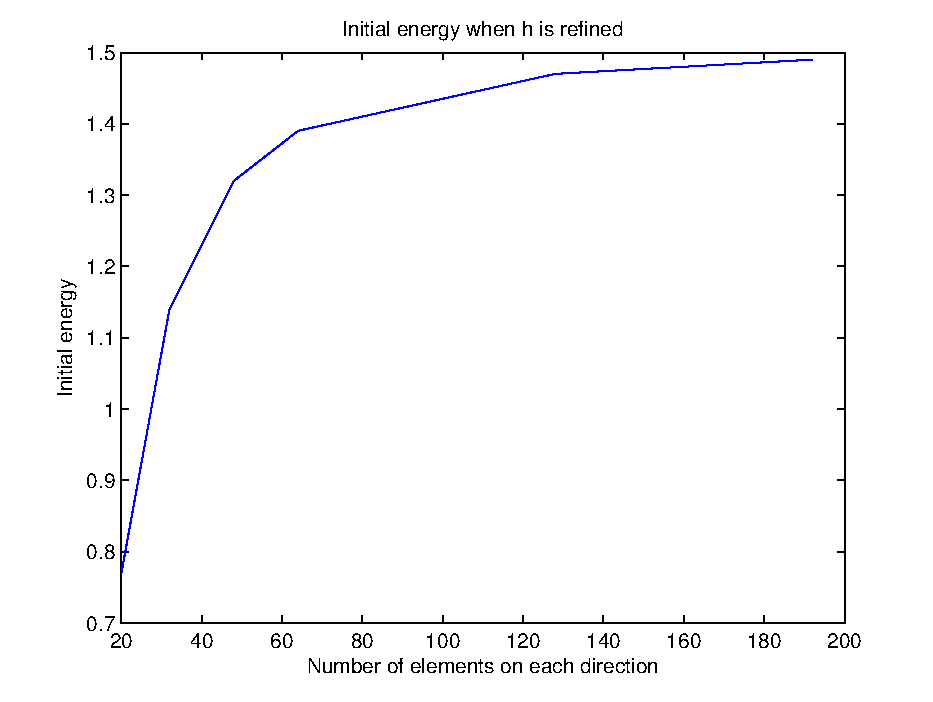
\includegraphics[width=0.5\textwidth]{Figures/Chapter4/DHIT/Initial_ene}
	\caption{Initial energy evolution refining the mesh}
	\label{fig:initial_ene}
\end{figure}

Knowing this behavior of the initial condition, it is difficult to draw conclusions comparing the simulations with a DNS like AGARD database, \cite{_selection_????}. In order to avoid this problem, we scale the initial condition in a such way that its initial energy achieve the desired value. This has been done multiplying the initial condition by a factor defined as
$$\u_{0_{new}}=\sqrt{\frac{E_{0_{new}}}{E_{0_{old}}}}\u_{0_{old}},\quad\quad\mbox{where $E_{0_{new}}=1.5$}.$$

\subsubsection{Vorticity}
As an introductory result, we show the vorticity contour at two different time steps, $t=5.0\cdot10^{-3}$ and $t=2.0$. These results are obtained considering the nonlinear definition of $\a$ and the dynamic subscales tracking for the OSS method with a $64^3$ hexahedral trilinear elements mesh. 

In Figure \ref{fig:vorti_contour} we see that at the earlier time step the structures are much bigger than at $ t=2.0 $. As we will see in forthcoming sections, when the energy of the problem is dissipated, the energy containing eddies become smaller, reducing its vorticity. This mechanism induces a flattening of the energy spectra, as we will discuss later.
\begin{figure}[h!]
  \centering
  \subfigure[$t=5.0\cdot10^{-3}$]{\label{fig:vorti_contour_1}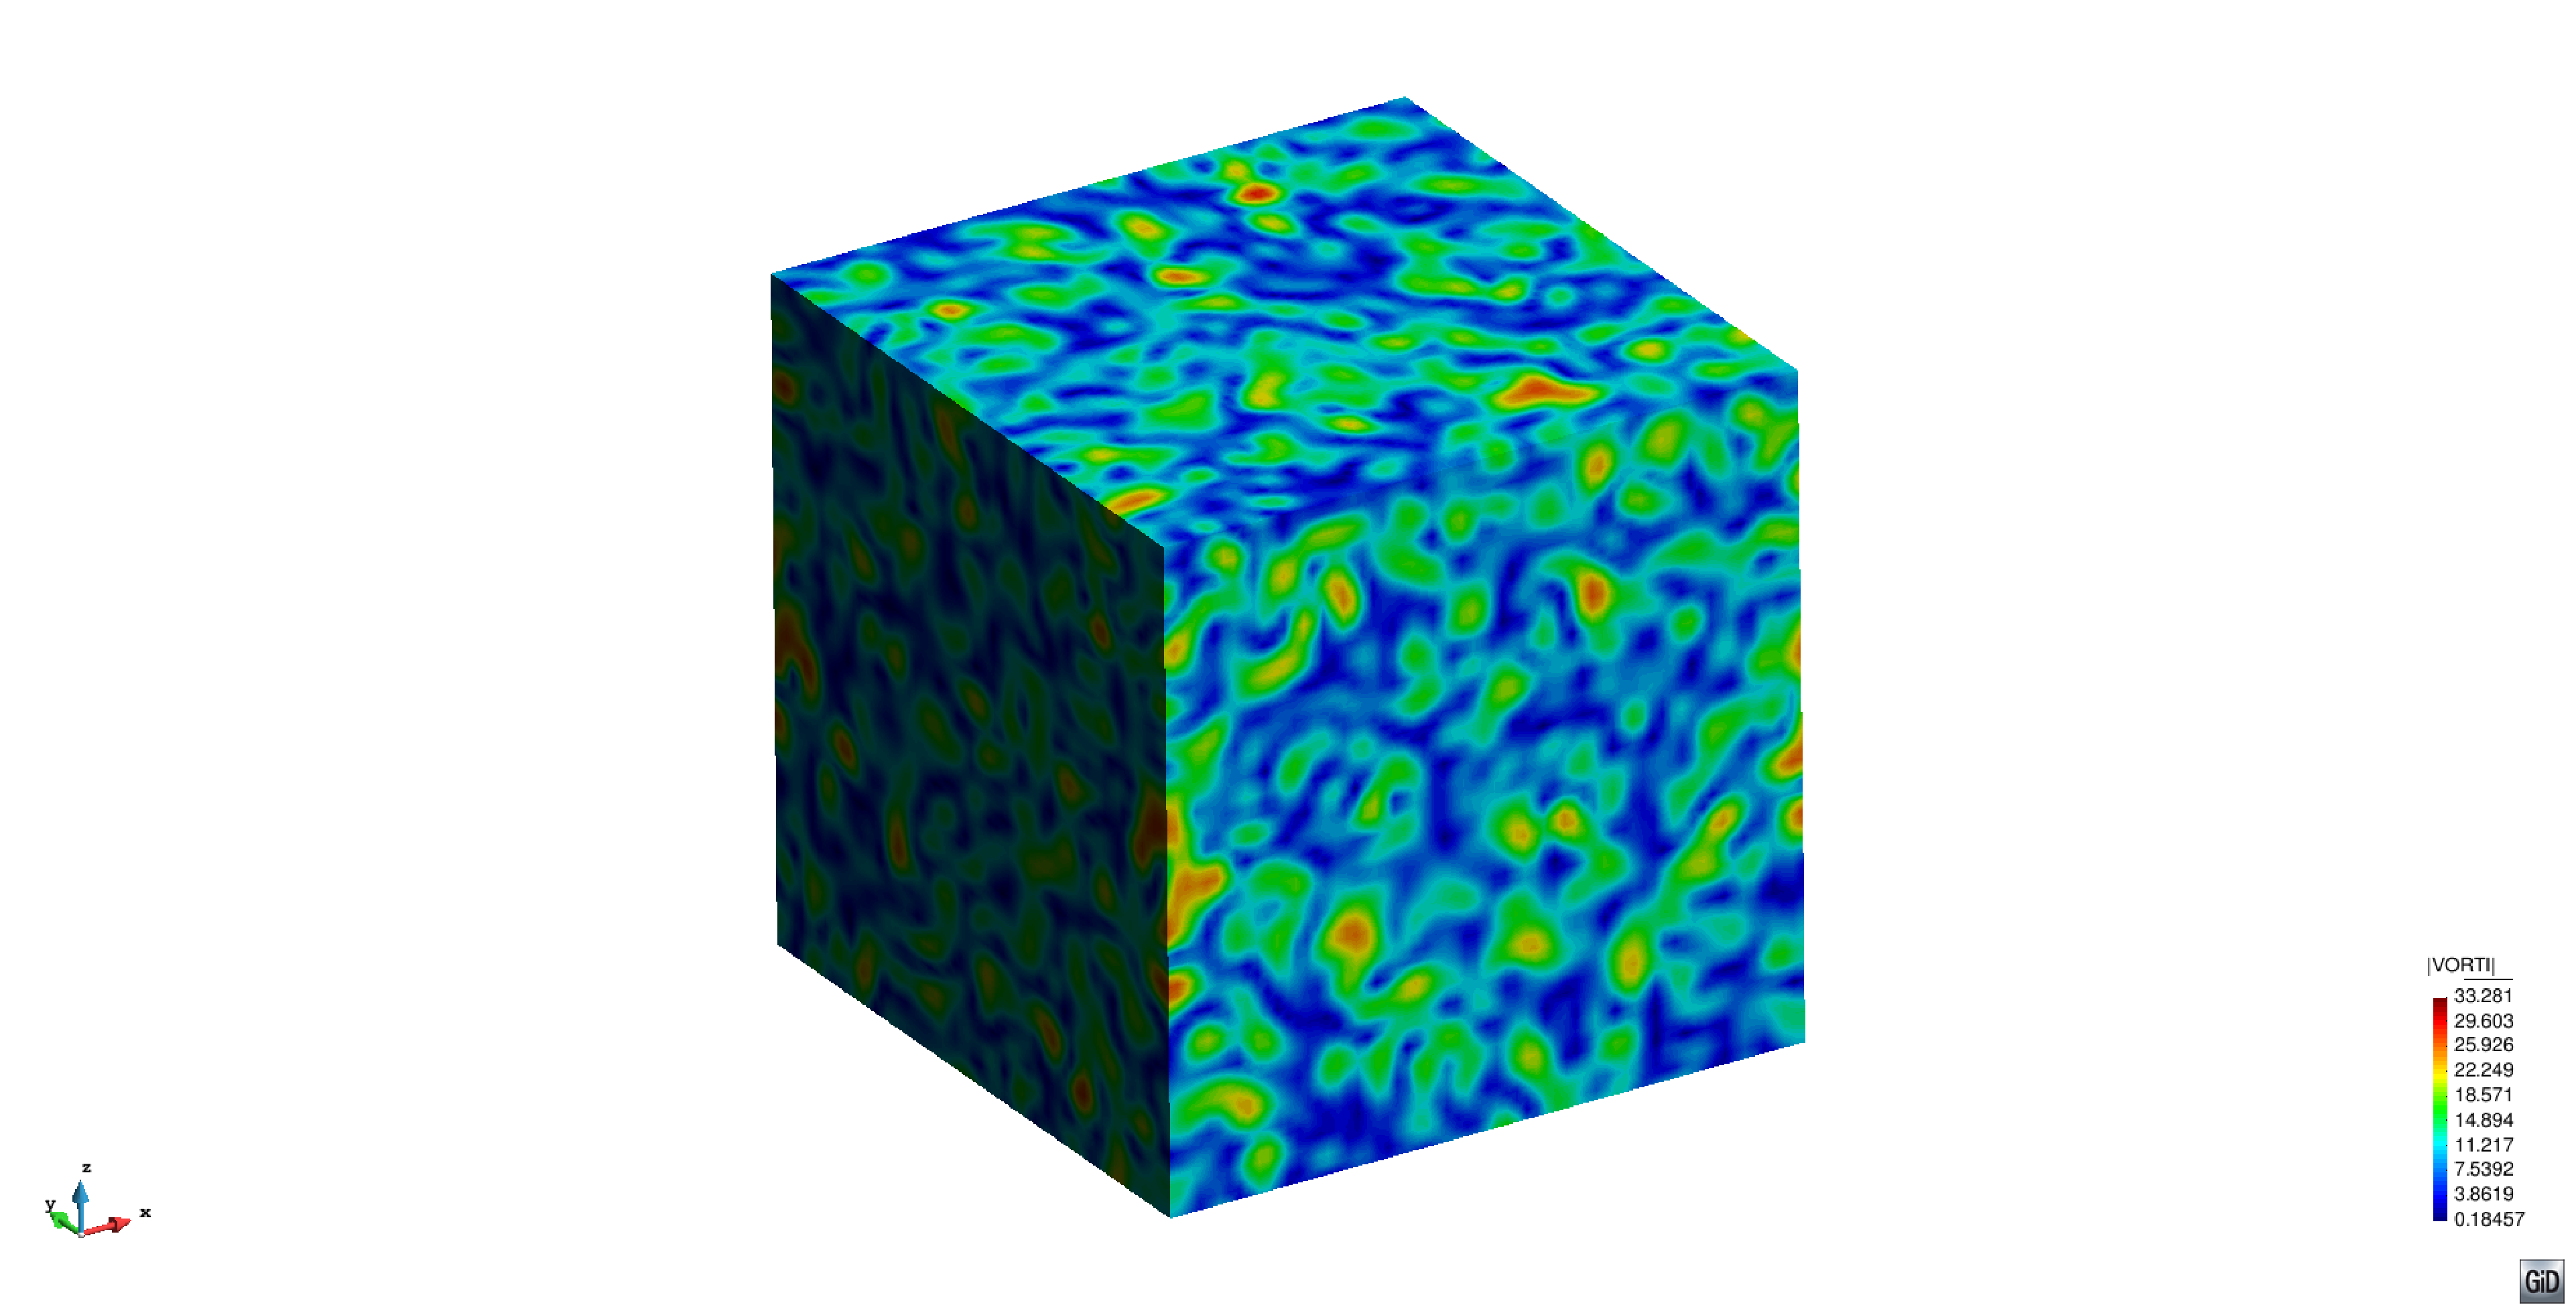
\includegraphics[clip=true, trim=18cm 2.25cm 18cm 2.25cm, width=0.49\textwidth]{Figures/Chapter4/DHIT/vorti_contour_1}}    
  \subfigure[$t=2.0$]{\label{fig:vorti_contour_2}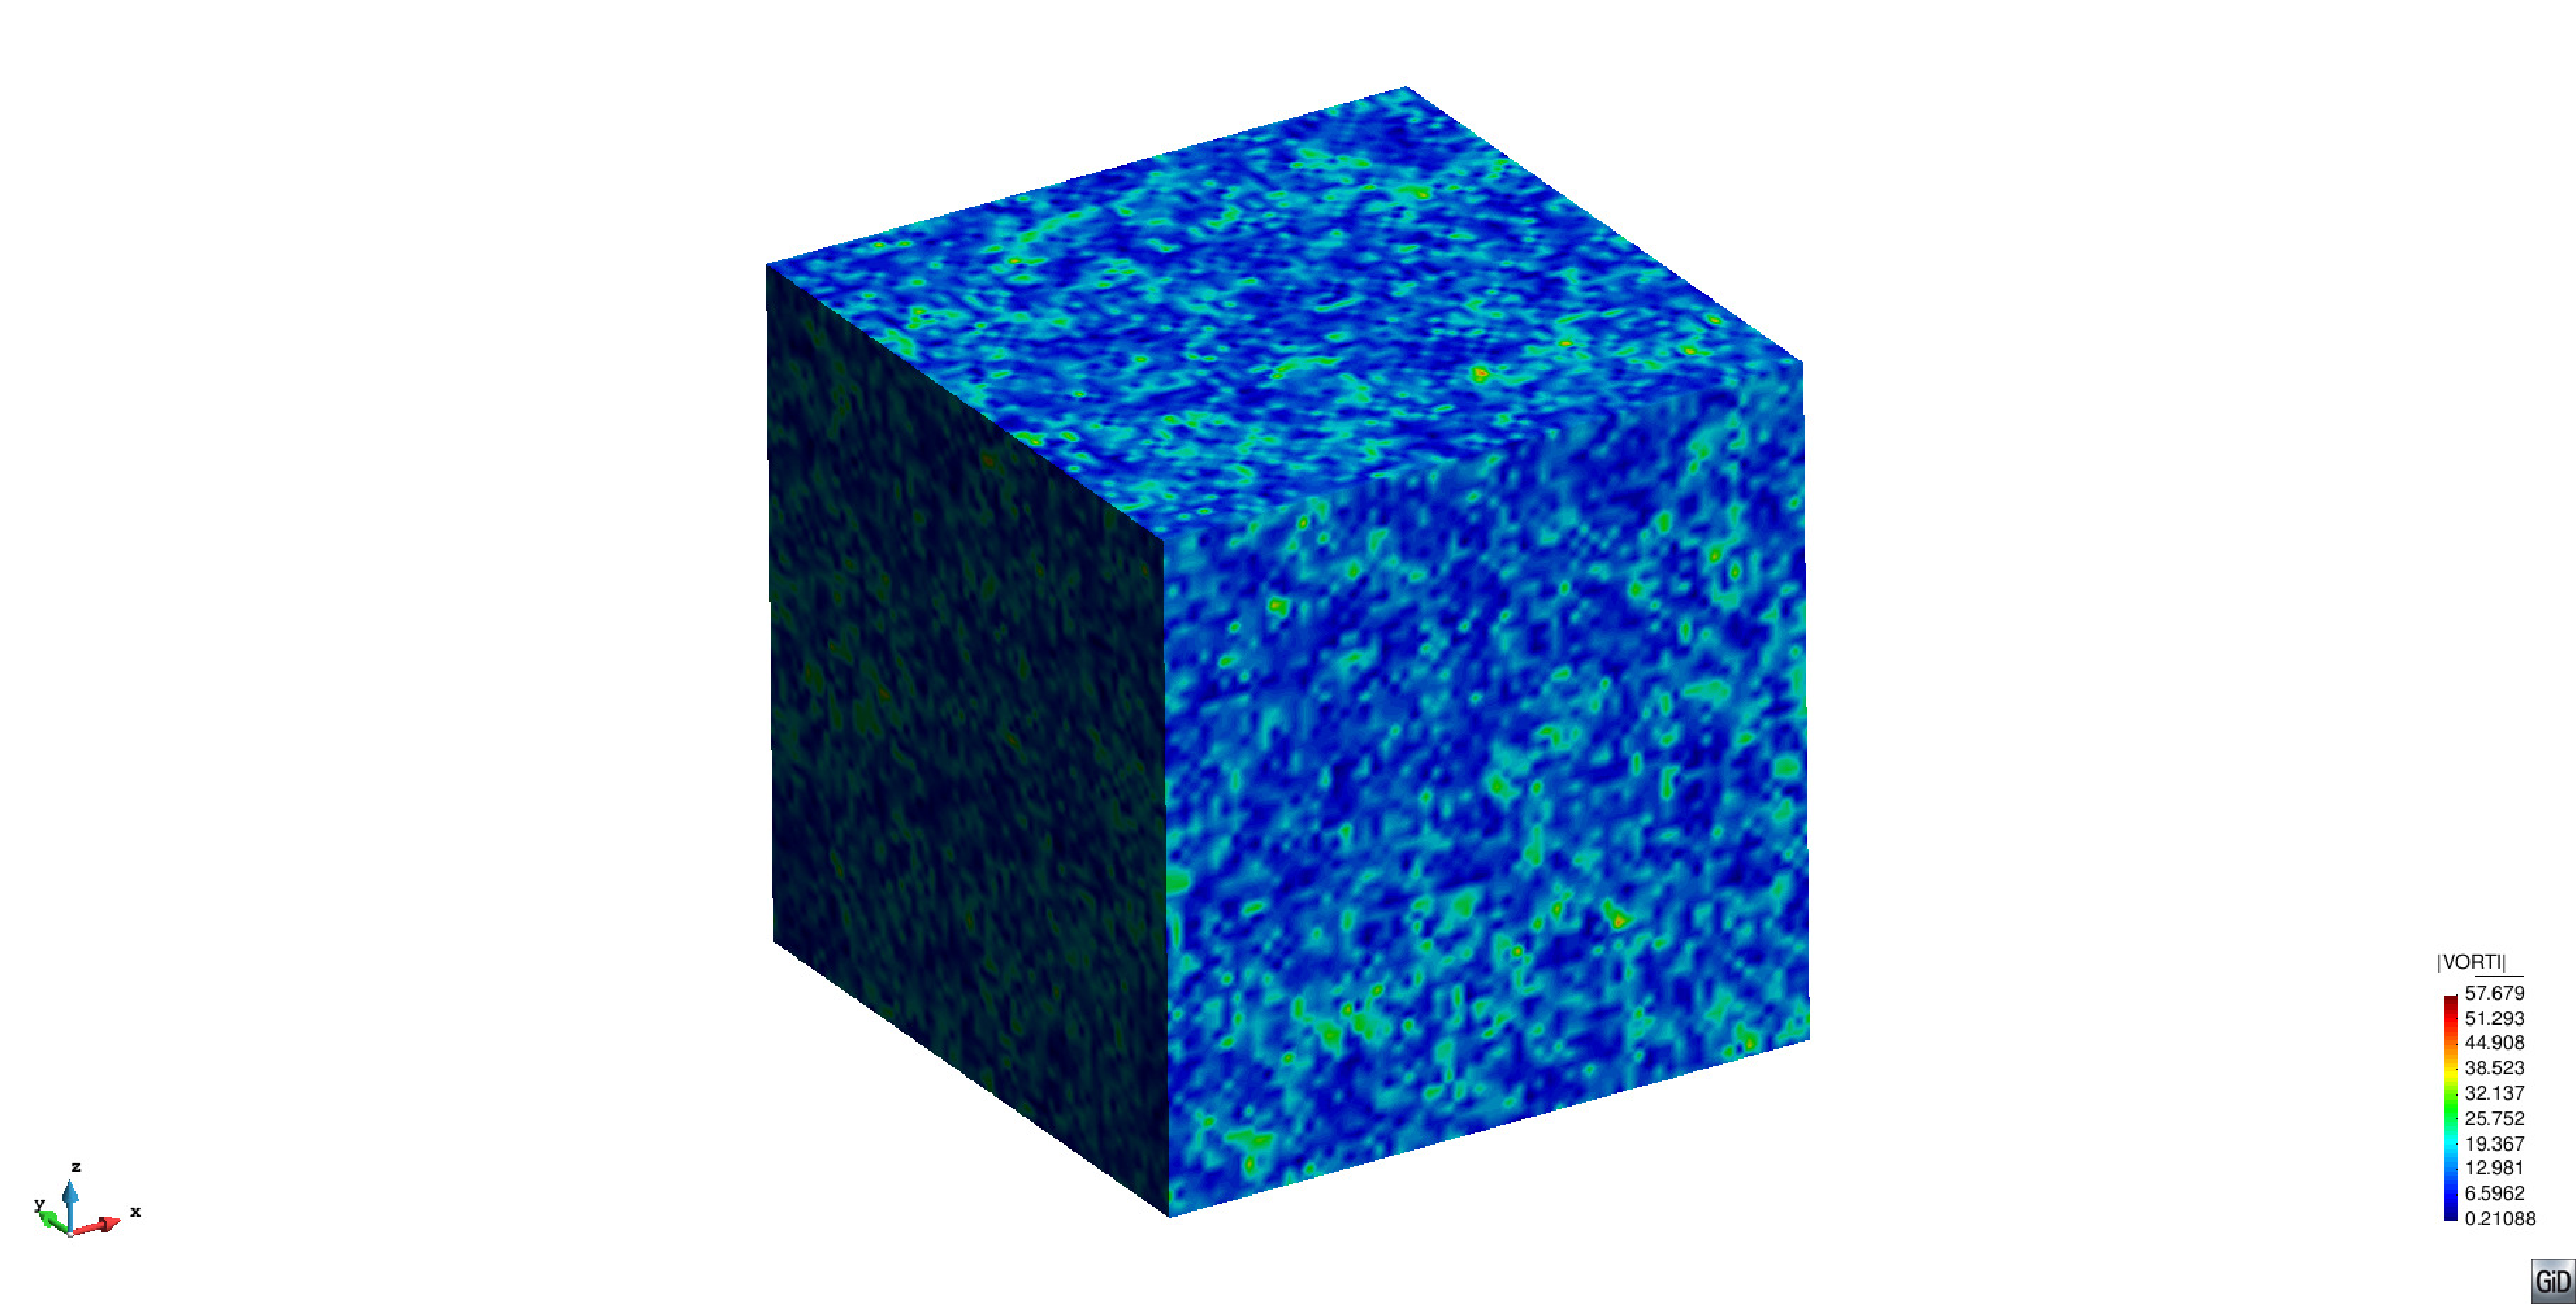
\includegraphics[clip=true, trim=18cm 2.25cm 18cm 2.25cm, width=0.49\textwidth]{Figures/Chapter4/DHIT/vorti_contour_2}}
  \caption{Vorticity contour}
  \label{fig:vorti_contour}
\end{figure}

\subsubsection{Energy Conservation}
\label{subsubsec-C4_ene_cons_DHIT}
% In order to check the conservation of energy of the problem and to ensure that the arguments developed at section \ref{sec-C4_energy} are correct, we evaluate each term for the DHIT test. Further, this type of test is excellent as a way to check the correct implementation of the method. 
% We show the results obtained solving the DHIT test in a $32^3$ elements mesh for the ASGS and OSS methods using the dynamic and nonlinear cases. 

In this section we present results of the energy budget described in Section \ref{sec-C4_energy} obtained in a $32^3$ elements mesh for the ASGS and OSS methods using the dynamic and nonlinear cases.
Fig. \ref{fig:ASGS_ene_balance_split} depicts the energy balance evolution for the mean flow equation (\ref{eq-C4_FE_balance2}) and the subscale equation (\ref{eq-C4_sgs_balance2}) separately for the Dyn-Nl-ASGS case. It can be seen that the variation of kinetic energy shown by the FE component in Fig. \ref{fig:ASGS_MF_balance} is offset in a large part by the transfer of energy to the subscales, while remaining energy on the mean flow balance is offset by the viscous term. On the other side, Fig.~\ref{fig:ASGS_ss_balance} shows that the energy transferred from the FE equation is mainly dissipated by the subscale velocity term. There is an small variation of the kinetic energy of the subscale at the beginning of the simulation. Note that since the viscosity is small, so are the viscous effects compared to the dissipation introduced by the subscale velocity. As we use a skew-symmetric form of the convective term, this term does not affect the energy balance and is not plotted in Fig. \ref{fig:ASGS_MF_balance}. Since $\tau_c=0$, the pressure subscale term $\tau_c^{-1}\|\tilde{p}\|^2
= \tau_c \Vert {\cal P}(\nabla\cdot\u_h)\Vert^2$ is also zero and does not appear in Fig.~\ref{fig:ASGS_ss_balance}.

\begin{figure}[h!]
  \centering
  \subfigure[Mean flow equation energy balance]{\label{fig:ASGS_MF_balance}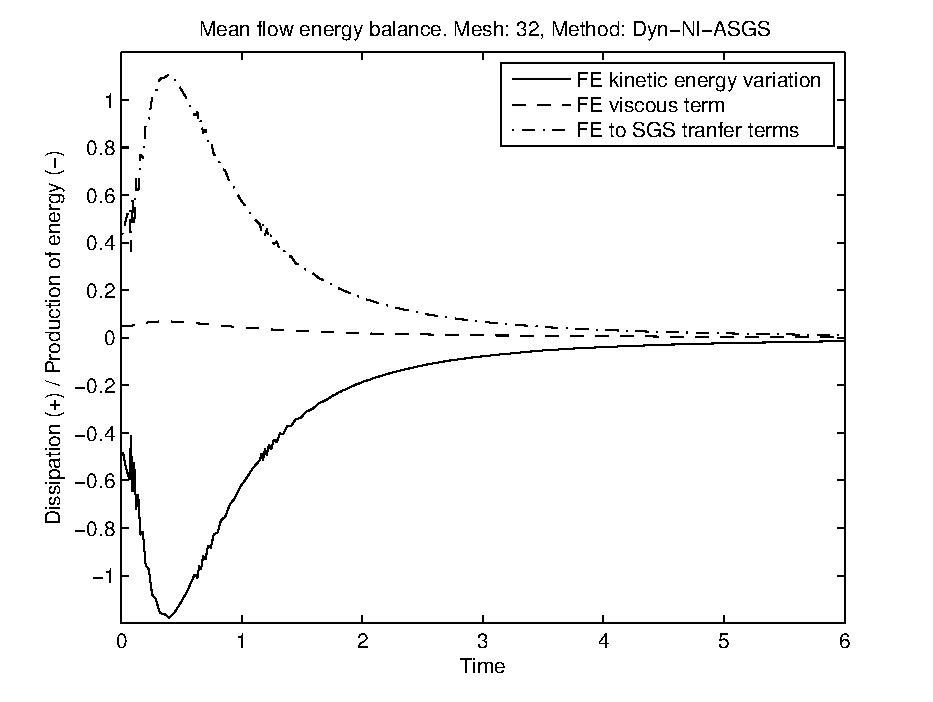
\includegraphics[width=0.49\textwidth]{Figures/Chapter4/DHIT/MF_ene_balance_ASGS_dyn_nl}}    
  \subfigure[Subscale equation energy balance]{\label{fig:ASGS_ss_balance}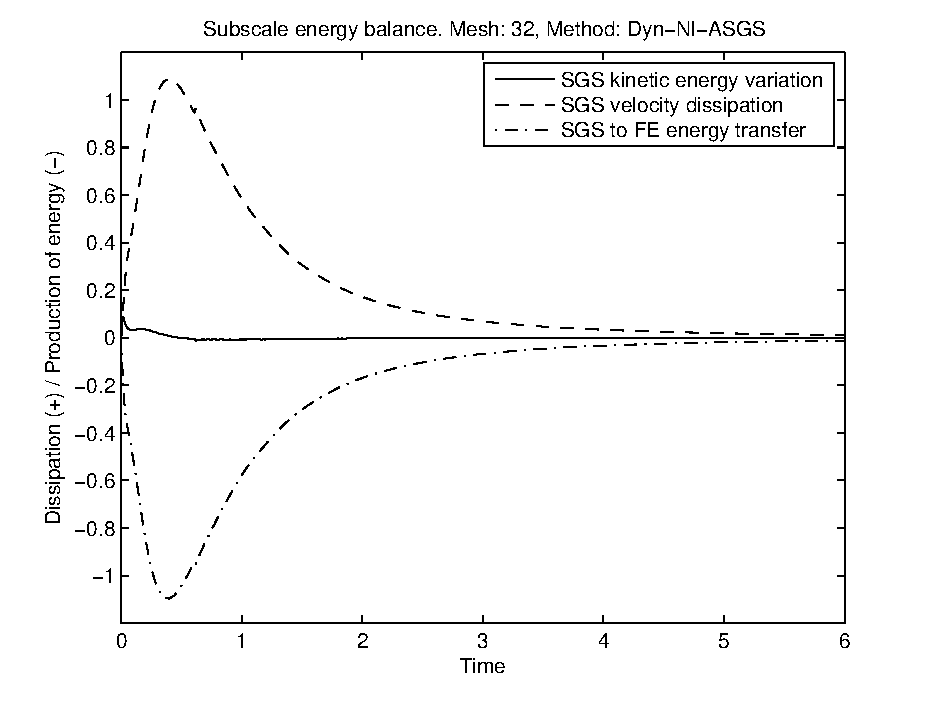
\includegraphics[width=0.49\textwidth]{Figures/Chapter4/DHIT/SS_ene_balance_ASGS_dyn_nl}}
  \caption{Mean flow and subscale energy balances for the Dyn-Nl-ASGS method.}
  \label{fig:ASGS_ene_balance_split}
\end{figure}

%Note that some oscillations in the FE time derivative term and FE to SS transfer terms
%can be observed in Fig. \ref{fig:ASGS_MF_balance}.{\color{blue}They can be explained by the coupling between temporal derivatives for the ASGS method in equation (\ref{eq-C4_time_deriv_ASGS}). No lo veo claro.}

%In order to check 
The energy balance evolution for the mean flow and the subscales equations in (\ref{eq-C4_FE_balance2})-(\ref{eq-C4_sgs_balance2}) for the Dyn-Nl-OSS case are shown in Fig. \ref{fig:OSS_ene_balance_split}. Fig. \ref{fig:OSS_MF_balance} depicts the energy balance evolution for the mean flow equation. Like for the ASGS method, the loss of kinetic energy is balanced by the FE scales to subscales energy transfer terms. The FE viscous term also has a very little impact on the dissipation of energy. On the other side, the subscales energy balance shown in Fig. \ref{fig:OSS_ss_balance} shows that almost all the energy transferred by the FE to the subscales is offset by the subscale velocity term,
again like in the ASGS method.
%by the subscale viscous term, also 
%like the ASGS method. Is important to say that the FE to SGS and SGS to FE energy transfer terms do not have any time derivative contribution, which do happen for the ASGS method. {\color{blue}This fact has a direct implication on the results since here, in the OSS method, there is no coupling between time derivative terms and we do not have oscillations.}
The only important difference between both methods is that \emph{no oscillations are observed in the FE kinetic energy evolution when the OSS method is used.}

\begin{figure}[h!]
  \centering
  \subfigure[Mean flow equation energy balance]{\label{fig:OSS_MF_balance}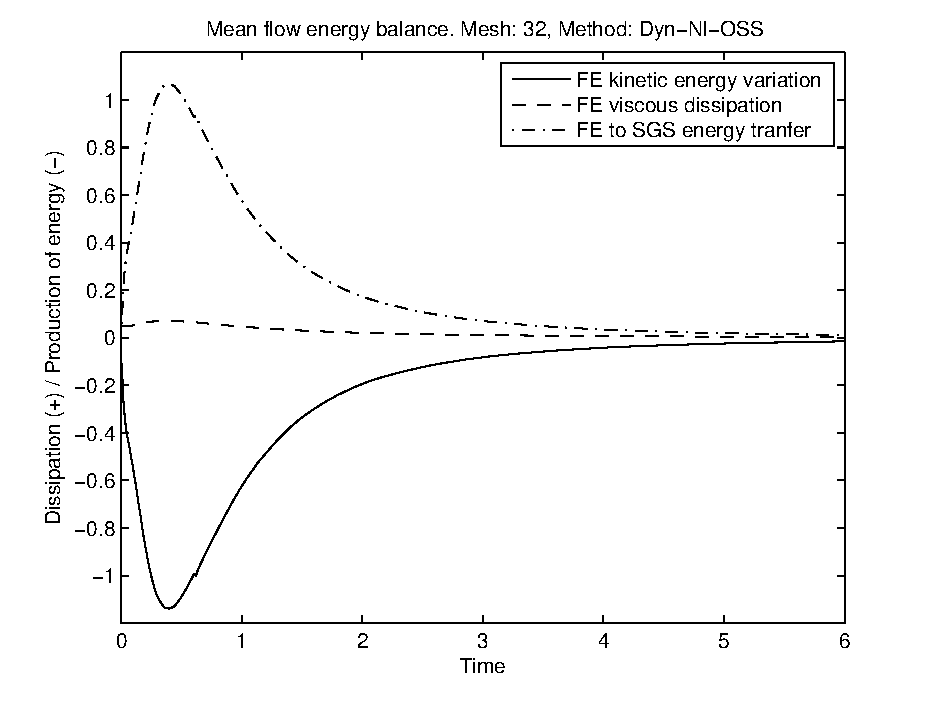
\includegraphics[width=0.49\textwidth]{Figures/Chapter4/DHIT/MF_ene_balance_OSS_dyn_nl}}    
  \subfigure[Subscale equation energy balance]{\label{fig:OSS_ss_balance}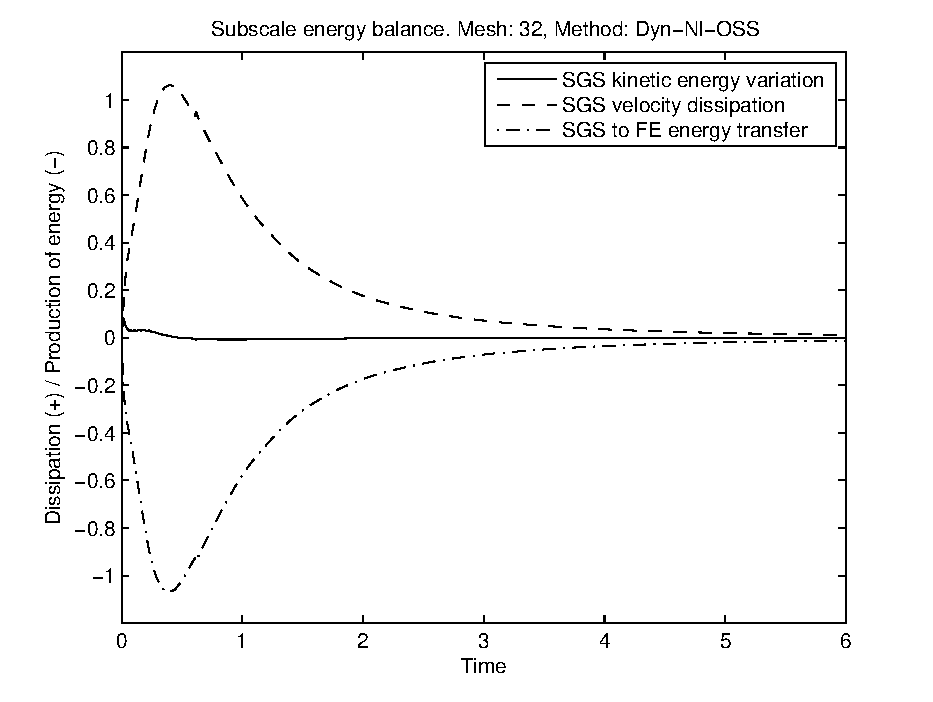
\includegraphics[width=0.49\textwidth]{Figures/Chapter4/DHIT/SS_ene_balance_OSS_dyn_nl}}
  \caption{Mean flow and subscale energy balances the Dyn-Nl-OSS method.}
  \label{fig:OSS_ene_balance_split}
\end{figure}

The global energy balance terms obtained solving the problem with the skew-symmetric convective term \textit{type 2} for the Dyn-Nl-ASGS and Dyn-Nl-OSS cases are shown in Fig. \ref{fig:ene_balance_sk2}. We note that the loss of skew-symmetry in the convective term has a non-negligible effect (see Figs.~\ref{fig:ASGS_ene_balance2} and \ref{fig:OSS_ene_balance2}). In particular, this term introduces negative dissipation (production of energy) into the problem. %As we will show in Section \ref{subsubsec-C4_Total_ene_DHIT}, 
This fact implies that the method is less dissipative and the energy decays at a slower rate than using the convective term \textit{type 1} and the method seems to be less diffusive. This negative contribution, however, is not predictable and could result in a blow up of the calculation. We refer to Section \ref{subsec-C4_effect_const} for further comments about numerical instabilities associated to the \textit{type 2} convective term.%Although no theoretical energy estimates are available we have not observed instabilities in practice.

\begin{figure}[h!]
	\centering	
	\subfigure[Global energy balance for Dyn-Nl-ASGS]{\label{fig:ASGS_ene_balance2}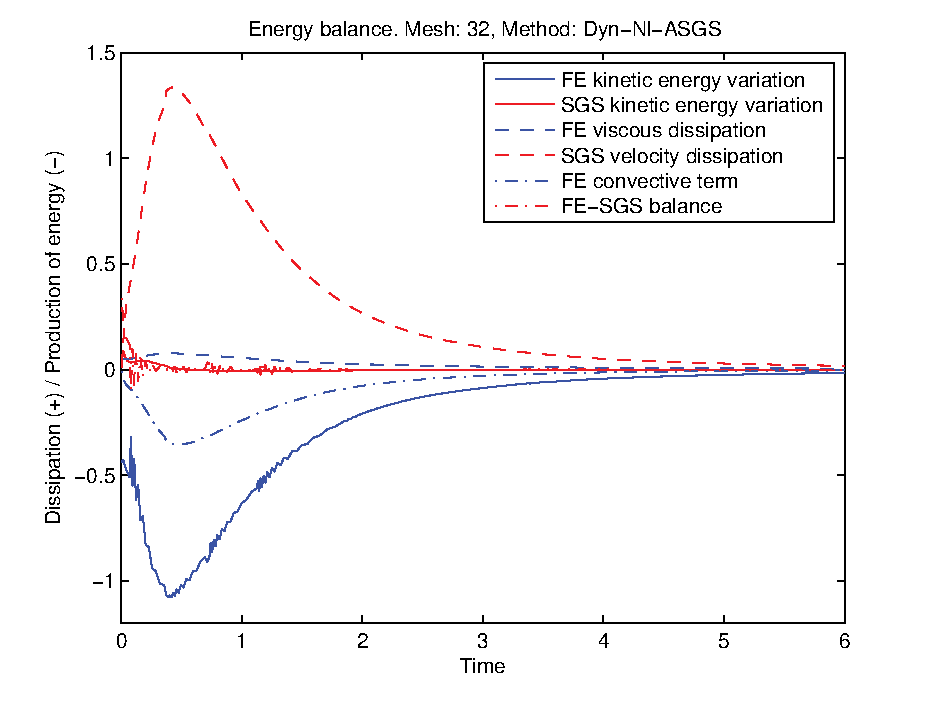
\includegraphics[width=0.49\textwidth]{Figures/Chapter4/DHIT/ene_balance_ASGS_sk2}}
	\subfigure[Global energy balance for Dyn-Nl-OSS]{\label{fig:OSS_ene_balance2}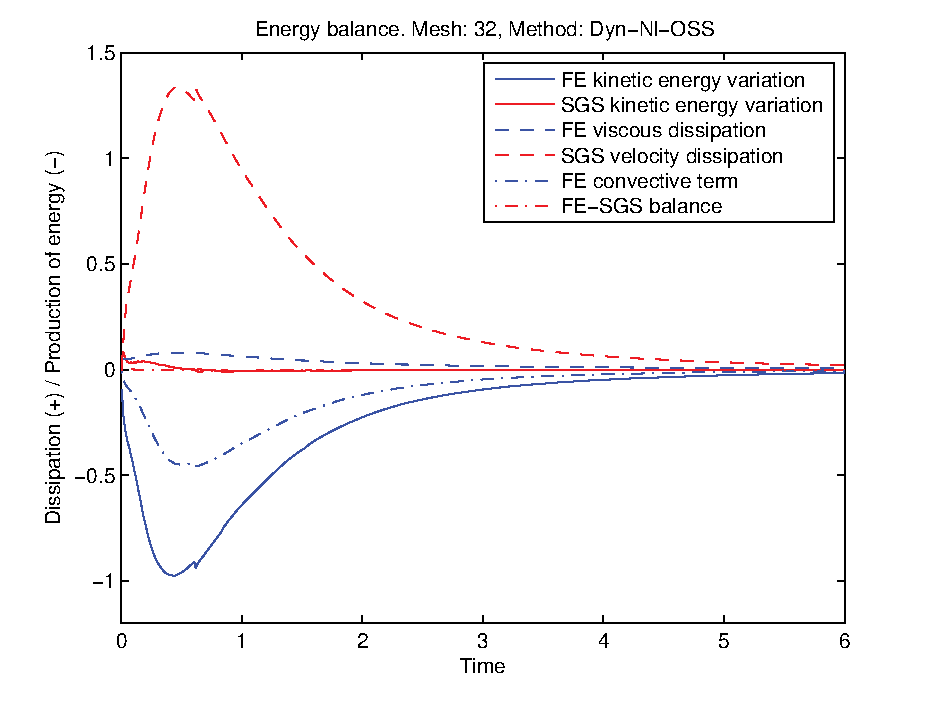
\includegraphics[width=0.49\textwidth]{Figures/Chapter4/DHIT/ene_balance_OSS_sk2}}
	\caption{Global energy balance using skew-symmetric convective term \textit{type 2}.}
	\label{fig:ene_balance_sk2}
\end{figure}

\subsubsection{Computational cost analysis}

\label{subsubsec-C4_comp_cost_DHIT}
The actual implementation in the parallel FE multiphysics code FEMPAR \cite{Badia2013a} is based on a classical domain decomposition strategy. At each nonlinear iteration the monolithic linear system is solved using a classical GMRES method applied to the Schur complement over the interfaces of the subdomains. This iterative procedure is preconditioned using a balancing Neumann-Neumann method applied to the monolithic system. The cost of each iteration is that of local Dirichlet solves for the Schur complement application and a local Neumann solve and a global solve for the preconditioner application (see \cite{mandel_balancing_1993,dohrmann_preconditioner_2003,badia_implementation_2013}). All local systems are solved using the sparse direct solvers in PARDISO library \cite{Schenk2004,Schenk2006}.

An important issue when comparing different computational methods is their corresponding computational cost. In order to characterize the performance of the different VMS methods introduced in Section \ref{sec-C4_prob_statement},  we analyze  some quantities that define the computational cost of each method, viz. nonlinear iterations, iterative solver iterations, and the adaptive time step evolution.

%All cases compared here have been solved using a $32^3$ linear hexahedral element mesh. This discretization is very coarse and it allows us to stress the differences between the proposed methods. In fact, due to this discretization, the linear and static ASGS case (Sta-Lin-ASGS) and the dynamic and linear ASGS case (Dyn-Lin-ASGS) do not converge at $t=0.0$ and  $t=0.123$, respectively; the nonlinear iterations diverge even reducing the time step size. Anyway, all the methods converge as $h\rightarrow0$.

The cases compared here have been solved using $32^3$ and $64^3$ linear hexahedral element meshes. The $32^3$ discretization is very coarse but it allows us to stress the differences between the proposed methods. In fact, due to this discretization, the linear and static ASGS case (Sta-Lin-ASGS) and the dynamic and linear ASGS case (Dyn-Lin-ASGS) do not converge at $t=0.0$ and  $t=0.123$, respectively; the nonlinear iterations diverge even reducing the time step size. Anyway, all the methods converge as $h\rightarrow0$.

%The Nonlinear iterations needed at each time-step is a good measure of the computational cost. It can be seen that the ASGS method requires less nonlinear iterations at each time step compared with OSS, in which the number of iterations are greater for all the cases. Referring to the OSS method, we see that the dynamic cases, both linear and nonlinear, needs less iterations to achieve convergence without any significant difference between each other.

The number of nonlinear iterations needed at each time step by the ASGS method is smaller than the one required by the OSS method in all cases. This is due to the evaluation of the projections at the previous nonlinear iteration $i-1$; the implicit treatment of the projection is carried out by the nonlinear loop. Alternatively, since the projection is a linear operation, it can be performed together with the linear system \cite{codina_analysis_2008}, although a more involved implementation is required. Referring to the OSS method, we observe that the dynamic cases, both linear and nonlinear, need less iterations to achieve convergence without any significant difference between each other.

However, the number of nonlinear iterations is not the most relevant measure of the computational cost as the cost of each iteration is not fixed when iterative linear solvers are considered. Fig. \ref{fig:com_cost_DHIT} shows the accumulated number of solver iterations for each time step for the methods that have attained convergence with the $32^3$ mesh (Fig. \ref{fig:soliter32}) and for the dynamic versions with the $64^3$ mesh (Fig. \ref{fig:soliter64}). 
%The amount of nonlinear iterations required at each time step is a good computational cost measure, but we do not know if the iterations between methods are equivalent. In order to have an idea of the global computational cost, we must have also into account the solver iterations. In Fig. \ref{fig:Soliter} we display the maximum number of solver iterations for each time step for the converged cases. 
%Unlike the nonlinear iterations, here we see that the ASGS method requires more solver iterations than OSS. The maximum solver iterations at each time step for the dynamic and nonlinear ASGS case is highly variable, with values from around 50 to around 270. Meanwhile, all cases of the OSS method seem to remain almost constant around 70.  
%{\color{blue}
Unlike the nonlinear iterations, here we see that the ASGS method requires more solver iterations than OSS. The maximum solver iterations at each time step for the dynamic and nonlinear ASGS case is variable, starting from near 600, dropping to 200 and rising to around 300 iterations at the end of the computation. Meanwhile, all cases of the OSS method remain almost constant, around 60 iterations in the dynamic cases and around 40 iterations in the static one. The relation between time step size and solver iterations for each method is analyzed in Section \ref{subsec-C4_small_time_step}. %}

\begin{figure}[h!]
	\centering	
	\subfigure[$32^3$ mesh]{\label{fig:soliter32}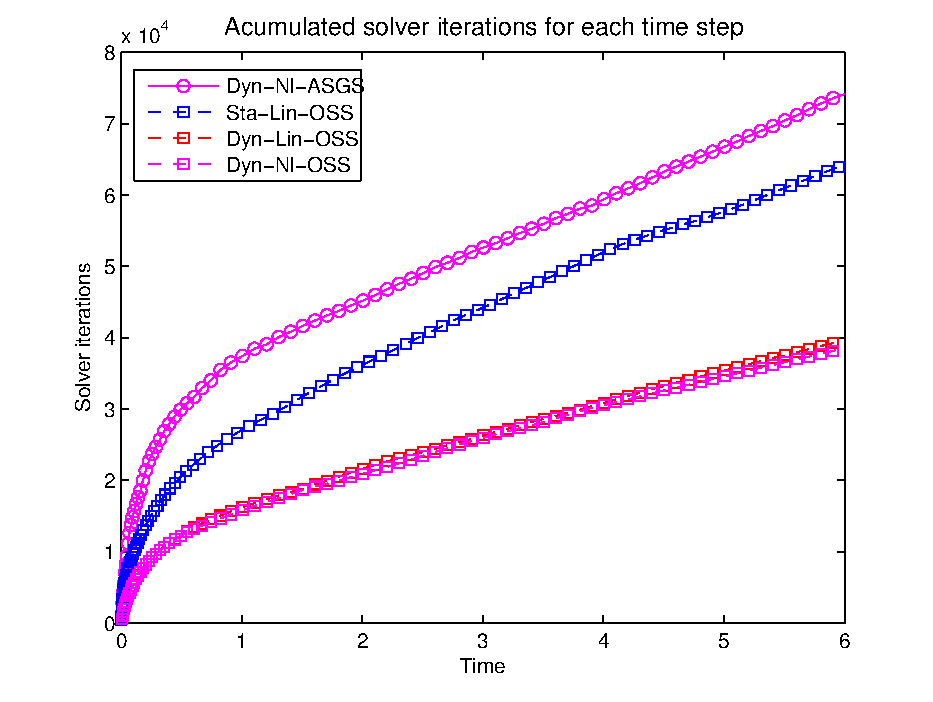
\includegraphics[width=0.49\textwidth]{Figures/Chapter4/DHIT/Acsoliter_32_scaled_cnvgd}}
	\subfigure[$64^3$ mesh]{\label{fig:soliter64}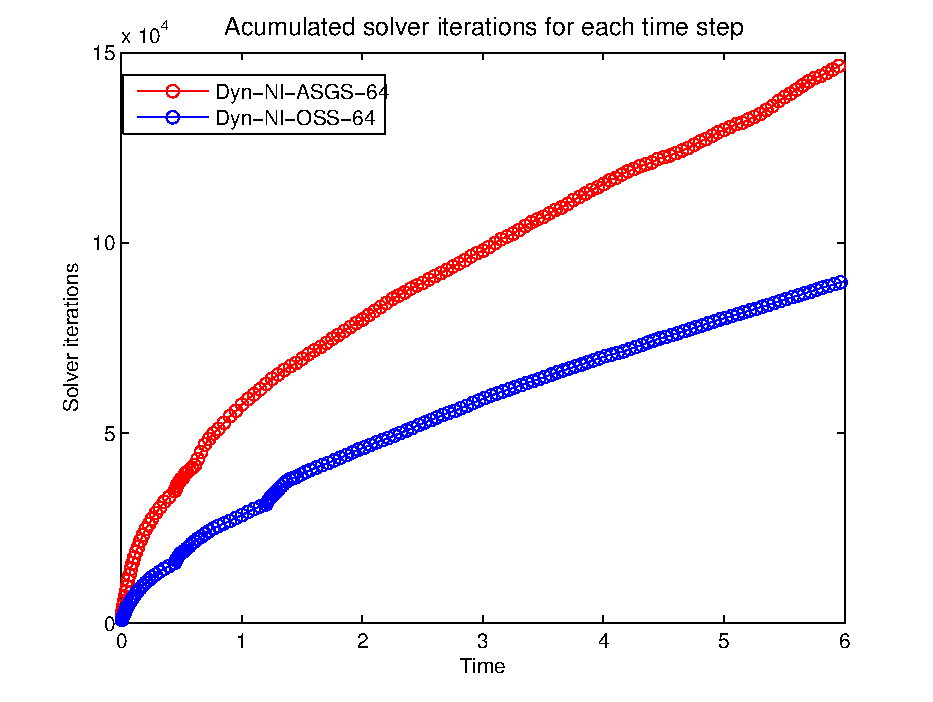
\includegraphics[width=0.49\textwidth]{Figures/Chapter4/DHIT/Acsoliter_64}}
	\caption{Accumulated solver iterations.}
	\label{fig:com_cost_DHIT}
\end{figure}

%The adaptive time stepping described in the previous subsection has an important role on the computational cost, as mentioned earlier. If the time step is reduced in order to ensure convergence, the global computational cost is increased. Then, we are looking for those methods that do not require time step reductions, consequently reducing the total amount of time step evaluations. There are some methods that need to reduce the time step to keep  convergence, which can be noticed  in Fig. \ref{fig:Soliter} by a sudden reduction of the solver iterations or in Fig. \ref{fig:Acsoliter} by the density of the points. It is seen in Fig. \ref{fig:com_cost_DHIT} that ASGS schemes perform worse than OSS counterparts in this respect. Comparing the dynamic and nonlinear cases for both methods, we see that ASGS needs to reduce more than twice the time step, while  OSS only twice. As it has been said before, the linear cases for ASGS, both static or dynamic, have not converged at certain time steps. In what refers to the linear cases for the OSS method, there is not any reduction of the time step, rather it is constantly increasing until the threshold.
%{\color{blue}
The adaptive time stepping described in the previous subsection has an important role on the computational cost, as mentioned earlier. If the time step is reduced in order to ensure convergence, the global computational cost is increased. Then, we are looking for those methods that do not require time step reductions, consequently reducing the total amount of time step evaluations. In this case, any of the methods shown in Fig. \ref{fig:soliter32} need to reduce the time step. Since we do not have any time step reduction and the number of solver iterations per step is stabilized after $t=1$ for the $32^3$ mesh and $t=1.5$ for the $64^3$ mesh, the total amount of accumulated solver iterations (in nonlinear and time loops) shown in Fig. \ref{fig:com_cost_DHIT} increases almost linearly. We see in this figure that the ASGS scheme performs worse than OSS in this aspect, with a steeper slope in both the  $32^3$ and the $64^3$ meshes. With respect to the OSS method, we see that the number of nonlinear iterations needed by the static version of this method results in a steeper slope of the accumulated solver iterations. No significant differences appear between the dynamic linear and nonlinear definitions of the OSS method.

Summarizing, ASGS methods need less nonlinear iterations (due to the treatment of the projections in the OSS method), but on the other hand  OSS methods need less solver iterations. Furthermore, \emph{ASGS formulations are prone to instabilities; linear formulations diverge and the nonlinear dynamic formulation requires much more solver iterations.}

We can clearly state that the most efficient method for this setting, in terms of computational cost, is the dynamic (both linear and nonlinear) OSS method; all OSS cases are below ASGS. It has to be said that the dynamic nonlinear OSS case requires less nonlinear iterations in some of the time step computations.
%}

\subsubsection{Total energy evolution}
\label{subsubsec-C4_Total_ene_DHIT}
In this section we present the total energy evolution of the resolved scales, i.e., the FE component. The results are shown in Fig. \ref{fig:total_ene} for the $32^3$ and the $64^3$ grids. We observe that all methods have a very similar accuracy for this test case, still far from the DNS result. The difference between the methods becomes even smaller when the mesh is refined and they are all closer to the DNS solution. Note that we do not plot the non-converged results from the ASGS static cases.

% SB: PUT A COMMENT?
%{\color{blue} Hay que pensar en el comentario que me hicieron en la ultima charla: no hay que comparar contra DNS sino contra DNS filtrado. Ver Sagaut secciones 9.1.1 and 9.2.1. }

\begin{figure}[h!]
	\centering	
	\subfigure[$32^3$ mesh]{\label{fig:total_ene_32}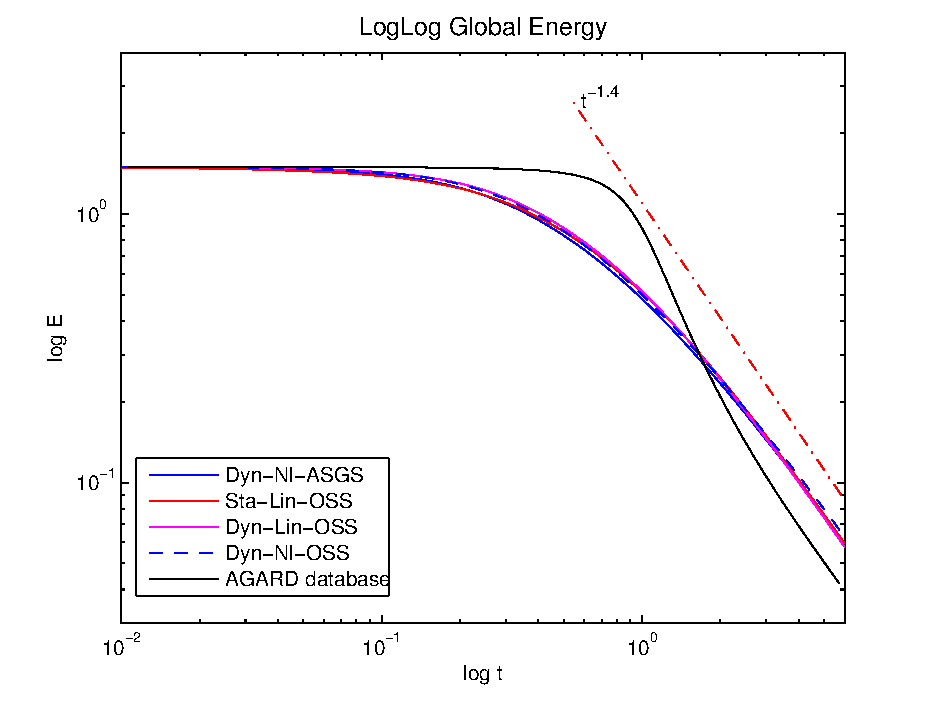
\includegraphics[width=0.49\textwidth]{Figures/Chapter4/DHIT/total_ene_32_scaled_loglog.pdf}}
	\subfigure[$64^3$ mesh]{\label{fig:total_ene_64}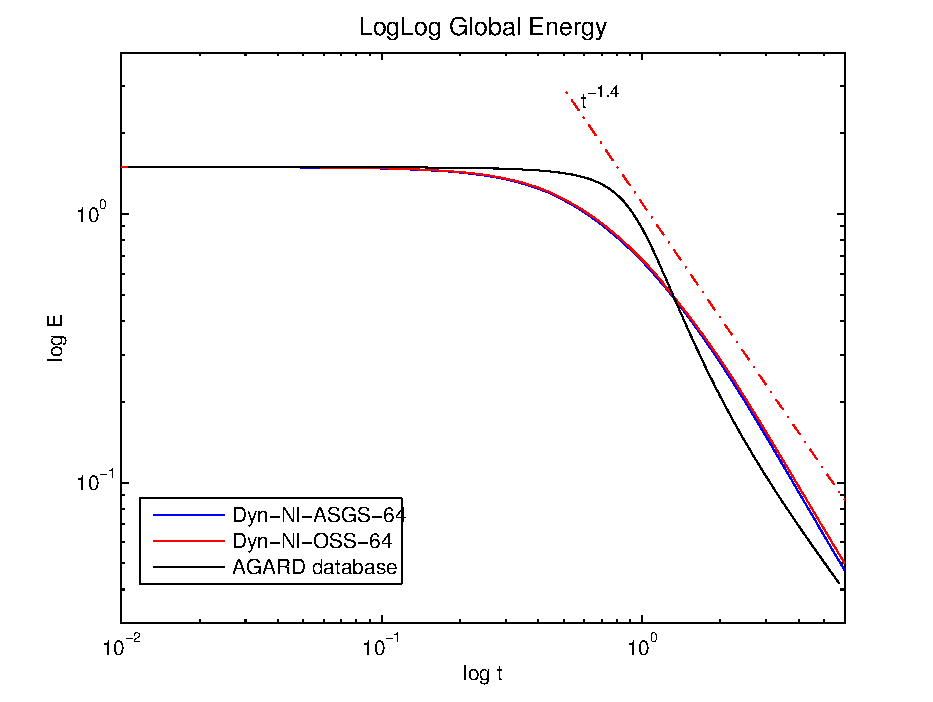
\includegraphics[width=0.49\textwidth]{Figures/Chapter4/DHIT/total_ene_64_scaled_loglog.pdf}}
	\caption{Total energy evolution for the $32^3$ and $64^3$ elements meshes with the scaled initial condition.}
	\label{fig:total_ene}
\end{figure}

\begin{remark}
\label{rem-C4_ene_skew2}
The results shown in Figure \ref{fig:total_ene} have been obtained using the skewsymmetric convective term \textit{type 1}, $b(\a,\u_h,\v_h)=\frac{1}{2}(\a\cdot\nabla\u_h,\v_h)-\frac{1}{2}(\mathbf{a}\cdot\u_h,\nabla\v_h)$. But what happens if we choose another definition for this term? We know that the nonskewsymmetric term (\textit{off}) can involve convergence problems. So we tested the influence of this term by solving the same problem with the convective skewsymmetric term (\textit{type 2)}. We did that for the dynamic and nonlinear cases for both methods, ASGS and OSS. The results obtained for this test are shown in Figure \ref{fig:ene_skew}.
\begin{figure}[h!]
	\centering	
	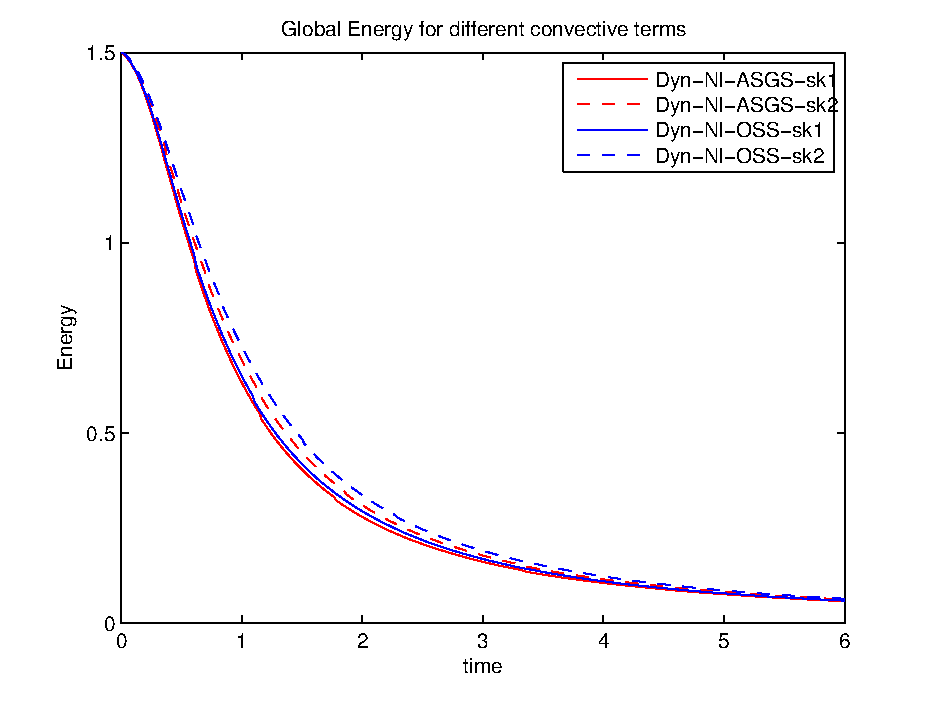
\includegraphics[width=0.5\textwidth]{Figures/Chapter4/DHIT/ene_skew_scaled}
	\caption{Total energy evolution. Comparison between different definitions for the convective term}
	\label{fig:ene_skew}
\end{figure}

We can clearly see in Figure \ref{fig:ene_skew} that the solution using the \textit{type 2} term is above the obtained with term \textit{type 1}. Then, we can say that the solution is less dissipative when we use this convective term. It has to be said that in Figure \ref{fig:ene_skew} we only represent the cases which exhibit more differences. In other words, in order to see the effect of the convective term definition, we only show the dynamic and nonlinear cases for ASGS and OSS methods. On the other hand, here we also have to take into account what we said on Remark \ref{rem-skewsym}. Introducing the nonlinearity on $\a$ we are increasing its weight on the convective term and changing its correct definition, therefore, it is normal that the differences between each definition increase.
\end{remark}

\subsubsection{Energy spectra}
According to \cite{mansour_decay_1994}, the resolution of the small scales in isotropic decaying turbulence is judged by the shape of the energy spectra at high wave numbers, and requires 
%that the total amount of wave numbers should be such that 
$k_{max}\eta\approx1$, $\eta=(\nu^3/\epsilon)^{1/4}$ being the Kolmogorov length scale and $k_{max}$ the maximum wave number required. In this case $k_{max}\approx182$, which means at least a $300^3$ FE mesh for a DNS computation, with a high computational cost.
%, so here it is shown the importance of a good LES method, which allow us to have good results on the energy containing eddies and the inertial subrange without solving the small scales.
%If we want to see if our VMS method is able to behave like a LES, we should be able to show that on the inertial subrange, the energy spectra follows the Kolmogorov law
%$$E(k)\propto\epsilon^{2/3}k^{-5/3}.$$
In this section we evaluate the capability of the VMS method to represent the energy of the  eddies at the inertial subrange without solving the small scales and compare the results against Kolmogorov's law prediction
$$E(k)\propto\epsilon^{2/3}k^{-5/3},$$
$E$ being the turbulent kinetic energy.

In Fig. \ref{fig:spec_32_64} the energy spectra for the different cases described in Table \ref{table:DHIT_cases}, using $32^3$ and $64^3$ linear hexahedral element mesh are presented. 
%Leaving aside the total energy evolution, which for this discretization is far to be considered acceptable, 
% {\color{blue}
We can see in Fig. \ref{fig:spec_32} that the energy spectra at $t=0.2$ decays with a different slope depending on the VMS method used. Although the differences are small and only appear at large wavenumbers, we see that the dynamic OSS models are less dissipative than the Dyn-Nl-ASGS and Sta-Lin-OSS ones. 
For the finer $64^3$ mesh the difference between the spectra obtained using Dyn-Nl-ASGS and Dyn-Lin-OSS are even smaller, as shown in Fig. \ref{fig:spec_64}; OSS is again less dissipative.
%The Dyn-Lin-OSS method seems to follow the $k^{-5/3}$ Kolmogorov law better at this time, but the Dyn-Nl-OSS case also have a good agreement with the Kolmogorov law for intermediate scales. %}

\begin{figure}[h!]
  \centering
  \subfigure[$32^3$ mesh]{\label{fig:spec_32}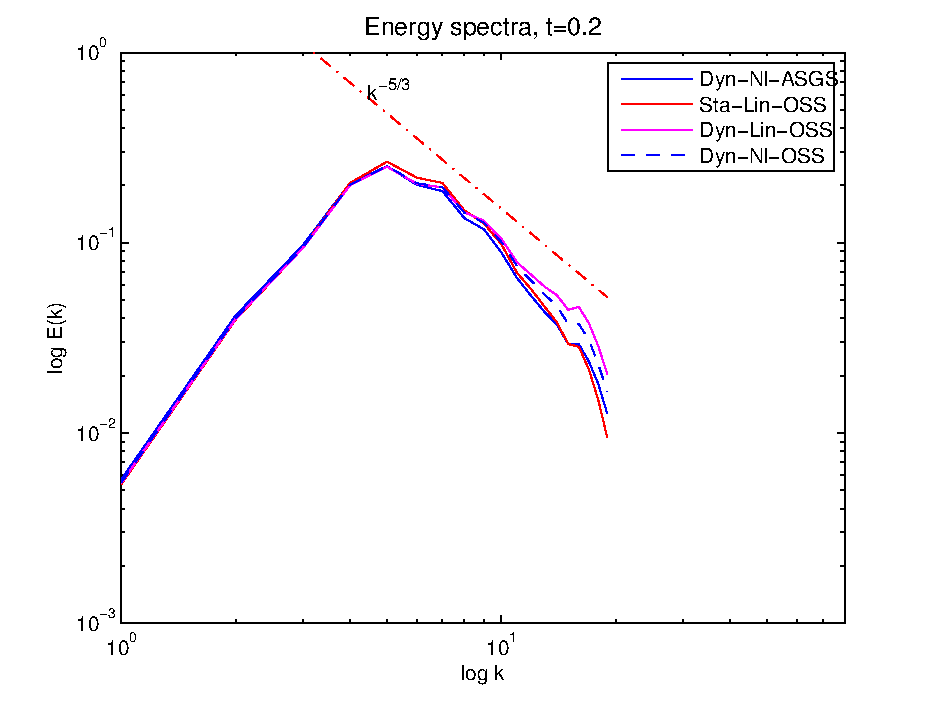
\includegraphics[width=0.49\textwidth]{Figures/Chapter4/DHIT/spec_32_02_scaled}}    
  \subfigure[$64^3$ mesh]{\label{fig:spec_64}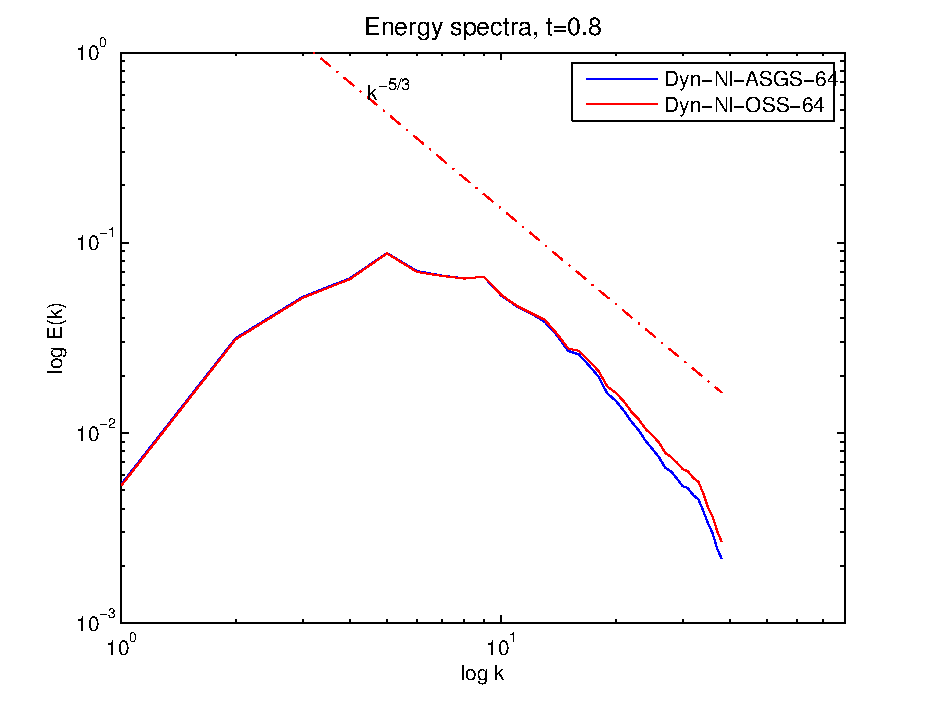
\includegraphics[width=0.49\textwidth]{Figures/Chapter4/DHIT/spec_64_08}}
  \caption{Energy spectra at $t=0.2$ ($32^3$ mesh) and $t=0.8$ ($64^3$ mesh).}
  \label{fig:spec_32_64}
\end{figure}

\subsubsection{$h$-$p$ refinement}

The energy decay computed using $32^3$ and $64^3$ linear FE meshes is far from the one obtained using DNS \cite{_selection_????}, as shown in Fig. (\ref{fig:total_ene}) and discussed above. To make clear that these poor results are due to this crude discretization,
%We have seen in Fig. \ref{fig:total_ene_32_sk1} that the total energy computed using a $32^3$ elements mesh is far from the one showed in the DNS \cite{_selection_????}. We also have said before that the initial total energy for this problem is highly mesh dependent. Thus, we expect that when we refine the mesh we will get a better initial energy approximation which will improve the whole energy evolution. Then, the results should become closer to the DNS.
%To check this assumption we perform 
we present a mesh refinement analysis, both reducing the element length $h$ and increasing the interpolation order $p$.
% (here $p$ is not the pressure field). 
We choose the Dynamic and Nonlinear OSS method (Dyn-Nl-OSS), which is the one that shows the lowest slope in the accumulated iterations evolution (Fig. \ref{fig:com_cost_DHIT}) for the $32^3$ and $64^3$ linear elements mesh. We solve the problem using the discretizations exposed in Table \ref{table:refinement}.

\begin{table}[h]
\centering
\begin{tabular}{ccc}
\toprule
Label&Mesh elements&Element type\\
\midrule
\midrule
32 ($Q$1)&$32^3$&hexahedral linear ($Q_1$)\\
64 ($Q$1)&$64^3$&hexahedral linear ($Q_1$)\\
128 ($Q$1)&$128^3$&hexahedral linear ($Q_1$)\\
32 ($Q$2)&$32^3$&hexahedral quadratic ($Q_2$)\\
64 ($Q$2)&$64^3$&hexahedral quadratic ($Q_2$)\\
32 ($Q$3)&$32^3$&hexahedral cubic ($Q3$)\\
\bottomrule
\end{tabular}
\caption{$h$-$p$ refinement cases.}
\label{table:refinement}
\end{table}

%To check this assumption we can refine the mesh in two different ways. On one hand, we can decrease $h$, that is to increase the number of mesh elements for each direction. On the other hand, we can use higher order elements, e.g. $Q_2$ or $Q3$. We do this analysis using the Dynamic and Nonlinear OSS method (Dyn-Nl-OSS), which is the one that shows the best results for the $32^3$ linear elements mesh. We solve the problem using the following discretizations:
%\begin{itemize}
%\item[-] $32^3$ hexahedral trilinear elements ($Q_1$).
%\item[-] $64^3$ hexahedral trilinear elements ($Q_1$).
%\item[-] $128^3$ hexahedral trilinear elements ($Q_1$).
%\item[-] $32^3$ hexahedral triquadratic elements ($Q_2$).
%\item[-] $64^3$ hexahedral triquadratic elements ($Q_2$).
%\item[-] $32^3$ hexahedral tricubic elements ($Q3$).
%\end{itemize}

In Fig. (\ref{fig:ene_hp}) we show the total kinetic energy evolution obtained using the discretizations defined in Table \ref{table:refinement}. Reducing the mesh size $h$ and/or increasing the polynomial order $p$ (not to be confused with the pressure) the result becomes closer to the DNS, as expected. In Fig. \ref{fig:ene_hp_close} three groups can be clearly observed, namely 32 ($Q$1), 32 ($Q$2) and 64 ($Q$1) and the remaining three. The best results are obtained using $Q$2 elements although the difference is really small.
%The refinement on $h$ and $p$ not only has effect on the initial energy, but also on the time evolution. When we reduce $h$ or increase $p$ the total kinetic energy evolution becomes closer to the DNS one. It also must be said that the refinement on $p$ is more effective than the refinement on $h$, which is a consequence of the enrichment of the FE space that is achieved when we increase $p$. 

\begin{figure}[h!]
  \centering
  \subfigure[Total evolution]{\label{fig:ene_hp_global}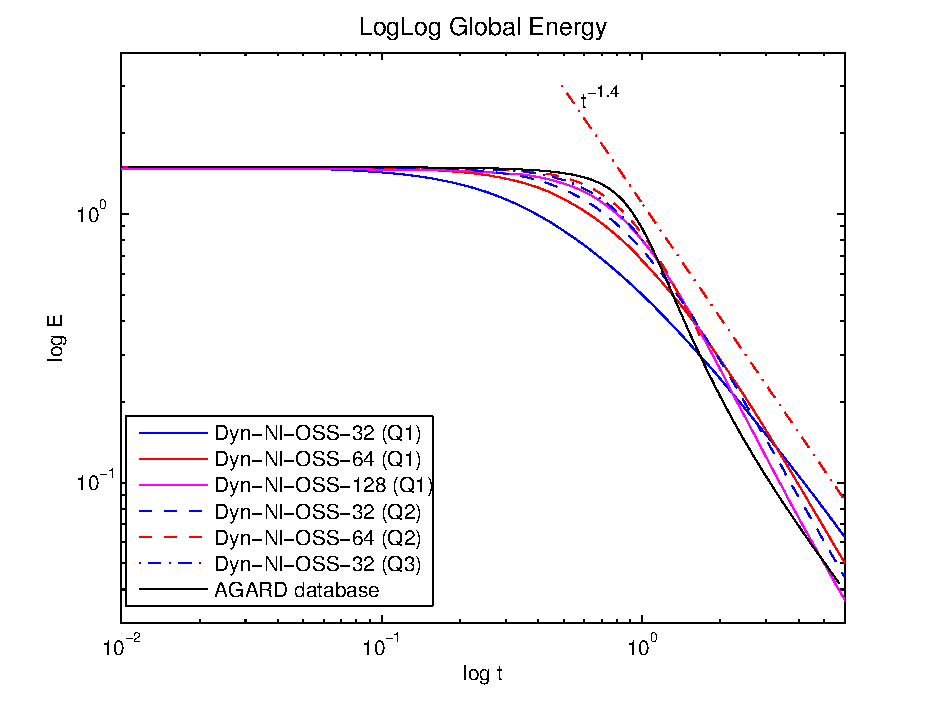
\includegraphics[width=0.49\textwidth]{Figures/Chapter4/DHIT/ene_hp_scaled_loglog}}    
  \subfigure[Close up view]{\label{fig:ene_hp_close}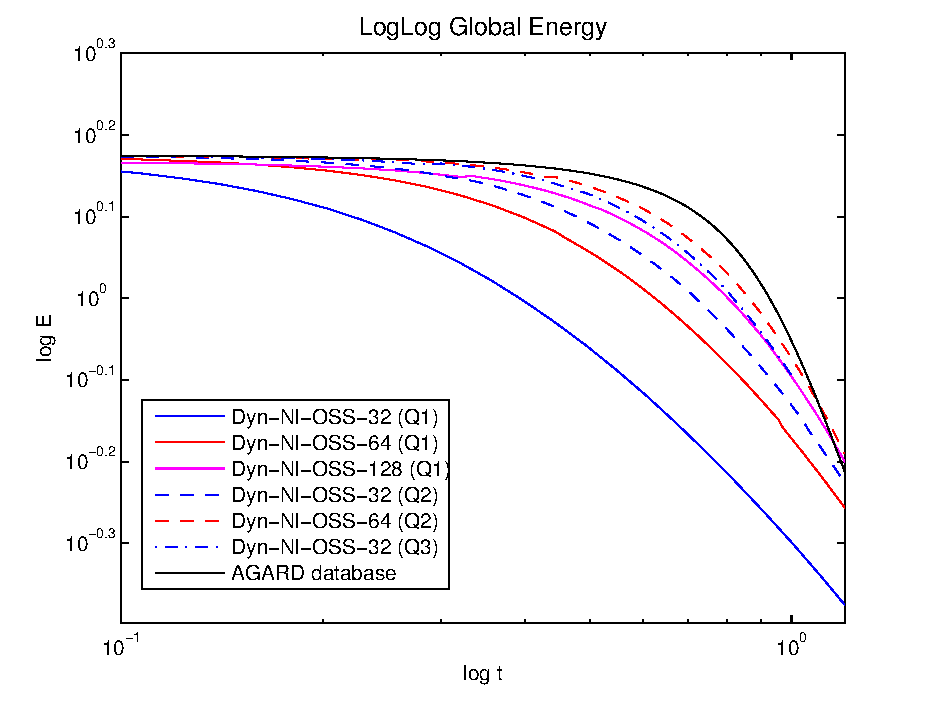
\includegraphics[width=0.49\textwidth]{Figures/Chapter4/DHIT/ene_hp_close_scaled_loglog}}
  \caption{Total kinetic energy evolution.}
  \label{fig:ene_hp}
\end{figure}

%With respect to the energy spectra, we expect to be related with the different kinetic energy evolutions showed in Fig. \ref{fig:ene_hp}. It means that if the total kinetic energy decays earlier, the energy spectrum must evolve to the $k^{-5/3}$ law earlier. If we think it on the opposite sense, that would suppose that the small scales are dissipating energy on a earlier stage, which implies a premature decaying of the total kinetic energy. In Fig. \ref{fig:spec_hp} we show the energy spectra at time $t=0.2$, $t=0.4$ and $t=0.8$ for the different cases presented before.

Given the differences in the total energy evolution the time at which the $k^{-5/3}$ law is achieved differs for the different methods. We show the energy spectra at time $t=0.8$ and $t=1.0$ for the different cases presented before in Fig. \ref{fig:spec_hp}. As it can be observed in Fig.~\ref{fig:spec_hp_08}, at $t=0.8$, only the energy spectra obtained using the 32 ($Q_1$) and  64 ($Q_1$) have a steeper slope, while the other cases are almost parallel to the $k^{-3/5}$ line. This is what was expected since the kinetic energy decay occurs earlier in the coarser cases.
%Effectively, we can see that the results in Fig. \ref{fig:spec_hp} performs as predicted by the total energy evolution. At Fig. \ref{fig:spec_hp_02}, $t=0.2$, the energy cascade for the case Dyn-Nl-OSS-32 ($Q_1$) is parallel to the $k^{-3/5}$ line, while the other cases still preserve the energy on the low wavenumbers. This behavior is consistent with the results shown in Fig. \ref{fig:ene_hp}, where the total kinetic energy for the case Dyn-Nl-OSS-32 ($Q_1$) decays earlier than all the other methods.
%At $t=0.4$, as shown in Fig. \ref{fig:spec_hp_04}, the cases with $64^3$ nodes follow the $k^{-5/3}$ law but those cases with more nodes still have the energy on the large eddies and, on the other hand, the case with less nodes has dissipated a large part of it through small scales. Finally, Fig.\ref{fig:spec_hp_08} shows us that the energy spectra for those cases with a finer mesh has a proper energy cascade at $t=0.8$.
%{\color{blue}
%At $t=0.4$, as shown in Fig. \ref{fig:spec_hp_04}, the $32$ (Q_1) case has the right energy decay slope, while for the cases with more degrees of freedom the contribution of the small scales to the energy is still increasing. Finally, Fig.~\ref{fig:spec_hp_08} shows us that the energy spectra for all cases has a proper energy cascade.
%At $t=0.8$ all the cases present a proper energy spectra, as shown in Fig.~\ref{fig:spec_hp_08}.
In Fig. \ref{fig:spec_hp_1} we show the energy spectra at $t=1.0$, and compare it against the DNS spectrum from \cite{_selection_????} at the same time step. It can be observed that the results tend to the DNS one as we increase resolution, being the $64(Q_2)$ case the most accurate one.

Note that the DNS spectra is not present in Fig. \ref{fig:spec_hp_08} because it is not available in the database \cite{_selection_????} at this time step.

\begin{figure}[h!]
  \centering
  \subfigure[Energy spectra at $t=0.8$]{\label{fig:spec_hp_08}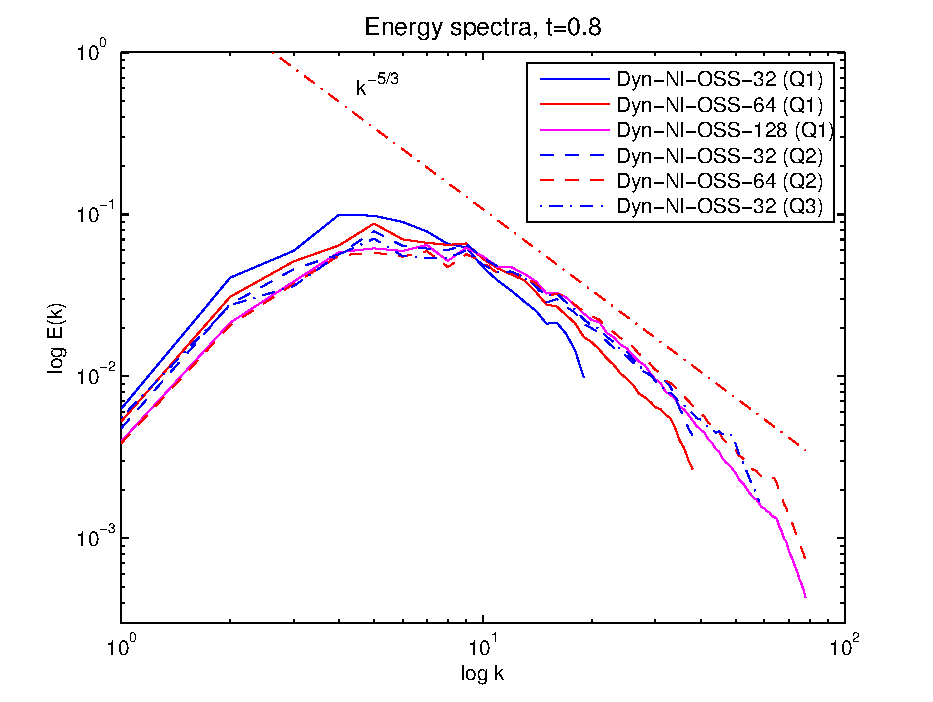
\includegraphics[width=0.49\textwidth]{Figures/Chapter4/DHIT/spec_hp_08}}
  \subfigure[Energy spectra at $t=1.0$]{\label{fig:spec_hp_1}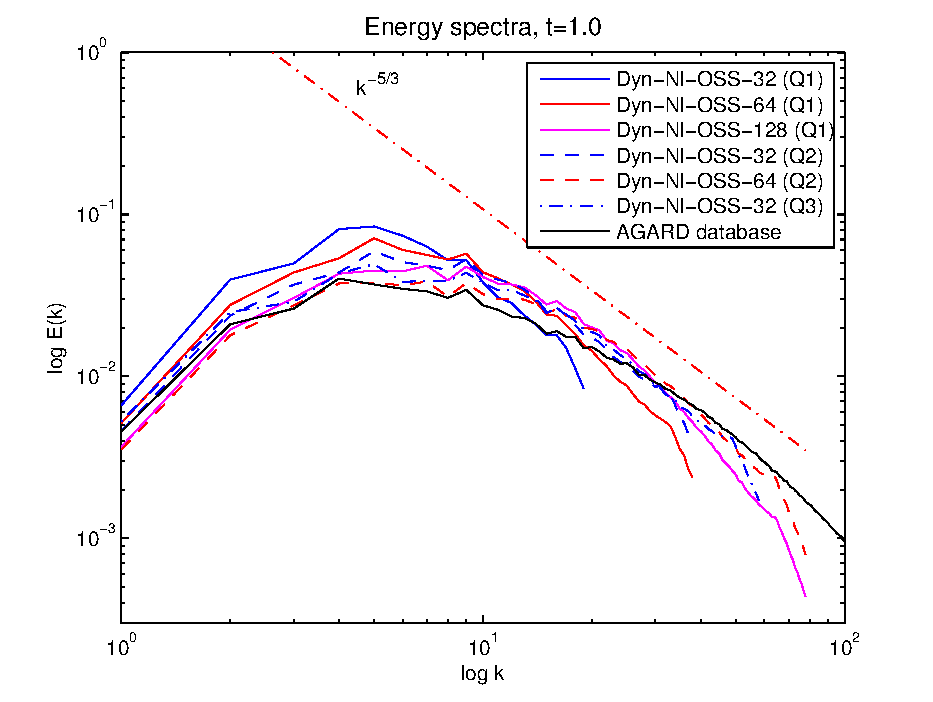
\includegraphics[width=0.5\textwidth]{Figures/Chapter4/DHIT/spec_hp_1}}
  \caption{Energy spectra at $t=0.8$ and $t=1.0$ for the $h$-$p$ refinement defined in Table~\ref{table:refinement}.}
  \label{fig:spec_hp}
\end{figure}

 \subsubsection{Comparison with a non-stabilized method}

% All the results presented up to this point have been computed using a VMS method, either ASGS or OSS. But, what would be the result using other methods? Are the methods presented here, comparable with classical LES methods? Which methods perform better? To answer all these questions, we have solved the problem adding a physical model without stabilization. To do that, an inf-sup stable element is needed and we have used the Taylor-Hood $Q_2/Q_1$ element. 
 %This element also has the unknowns at the nodes but uses shape functions of degree $2$ for the velocity degrees of freedom and shape functions of degree $1$ for the pressure DOFs. This type of element give stable results when we solve non convection dominated flows only taking into account the Galerkin terms.
 %We are solving a turbulent problem, so we must add a LES model to the Galerkin formulation in order to take into account the effect of the small scales on the flow when we solve it in a coarse mesh. 
 We use the classical static Smagorinsky model, consisting in adding a turbulent viscosity $\nu_t$ that depends on the velocity gradient and the characteristic element length $h$. This additional viscosity also acts as stabilization of convection, as usual in standard LES simulations. Then, we have to solve the standard Galerkin problem using Taylor-Hood $Q_2/Q_1$ elements and introducing a modified viscosity defined as
 \begin{equation}
 \label{eq-C4_nu_smago}
 \nu = \nu_l+\nu_t,
 \end{equation}
 where $\nu_l$ is the real flow viscosity and $\nu_t=(C_sh)^2|\nabla^s\u|$. $C_s$ is the Smagorinsky constant, which we set equal to $0.15$.

% In Fig. \ref{fig:ene_spec_q2q1} we show the total kinetic energy time evolution and the energy spectra of this method compared with the dynamic and nonlinear OSS method. In particular, we show the results for those cases from Table \ref{table:refinement} such that they have $65^3$ velocity nodes.
 We can see in Fig. \ref{fig:ene_q2q1} that the total kinetic energy is decaying faster for the non-stabilized method than for the OSS method. This behavior is directly related to the shape of the energy spectra in Figs. \ref{fig:spec_q2q1_02}-\ref{fig:spec_q2q1_08}, where we can see that the Smagorinsky method presents lower values of energy at $t=0.4$. It is important to point out the pile-up that appears in the Smagorinsky spectra, denoting that small scales are not dissipating energy properly.

\begin{figure}[h!]
   \centering
   \subfigure[Energy evolution]{\label{fig:ene_q2q1}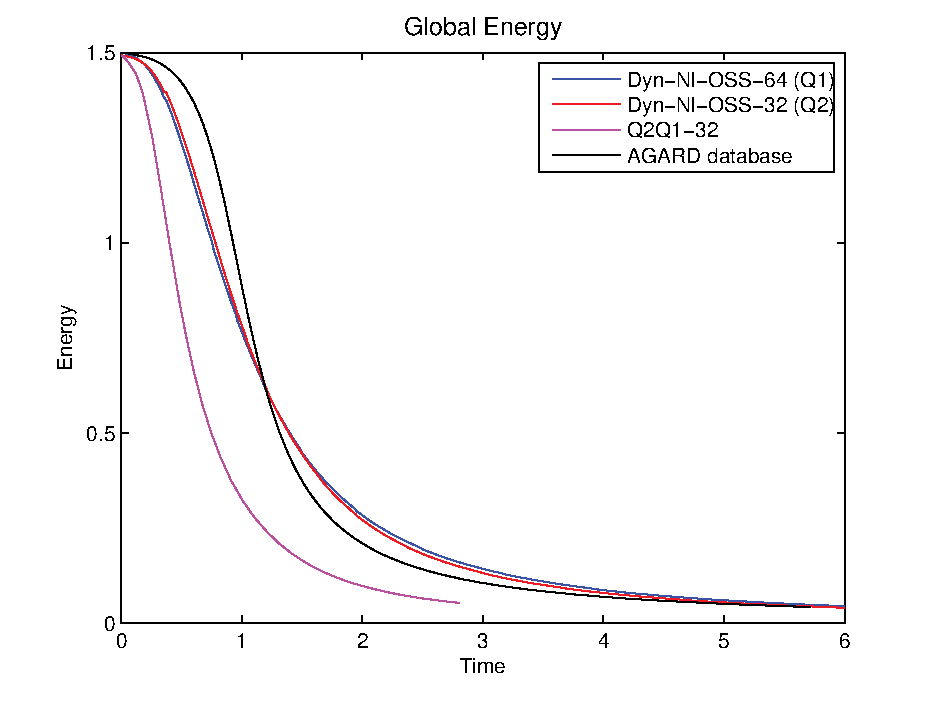
\includegraphics[width=0.49\textwidth]{Figures/Chapter4/DHIT/ene_q2q1_scaled}}  
   \subfigure[Energy spectra at $t=0.2$]{\label{fig:spec_q2q1_02}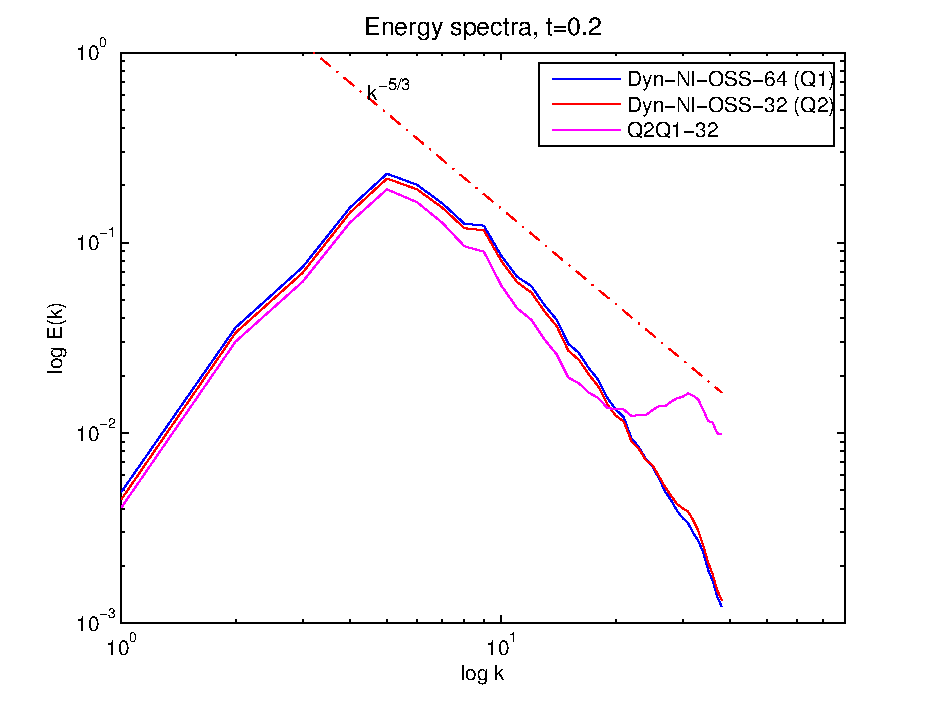
\includegraphics[width=0.49\textwidth]{Figures/Chapter4/DHIT/spec_q2q1_scaled_t02}}\\  
   \subfigure[Energy spectra at $t=0.4$]{\label{fig:spec_q2q1_04}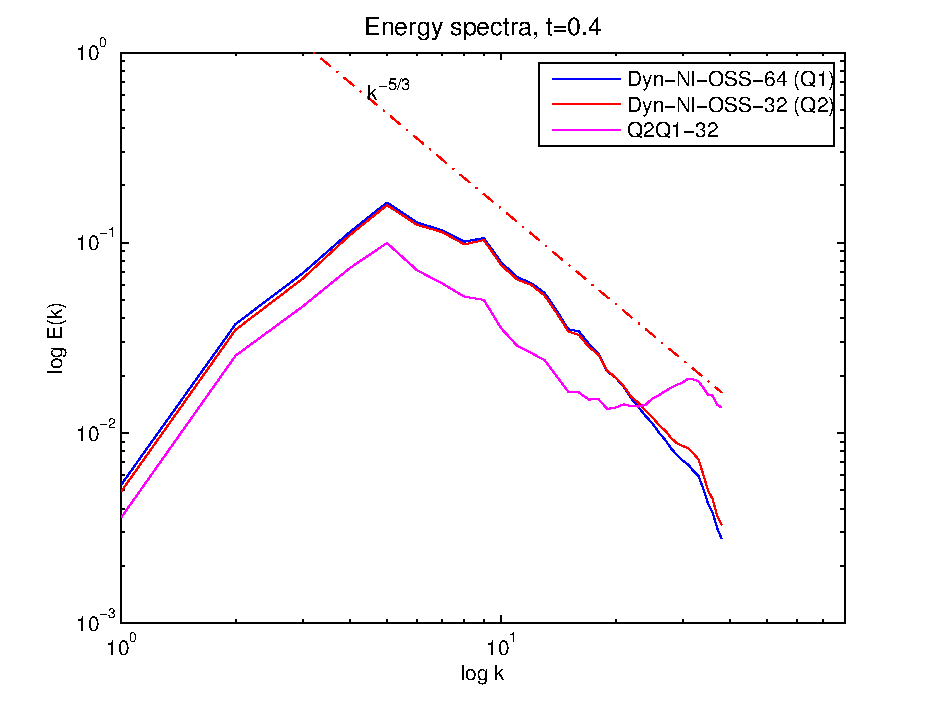
\includegraphics[width=0.49\textwidth]{Figures/Chapter4/DHIT/spec_q2q1_scaled_t04}}
   \subfigure[Energy spectra at $t=0.8$]{\label{fig:spec_q2q1_08}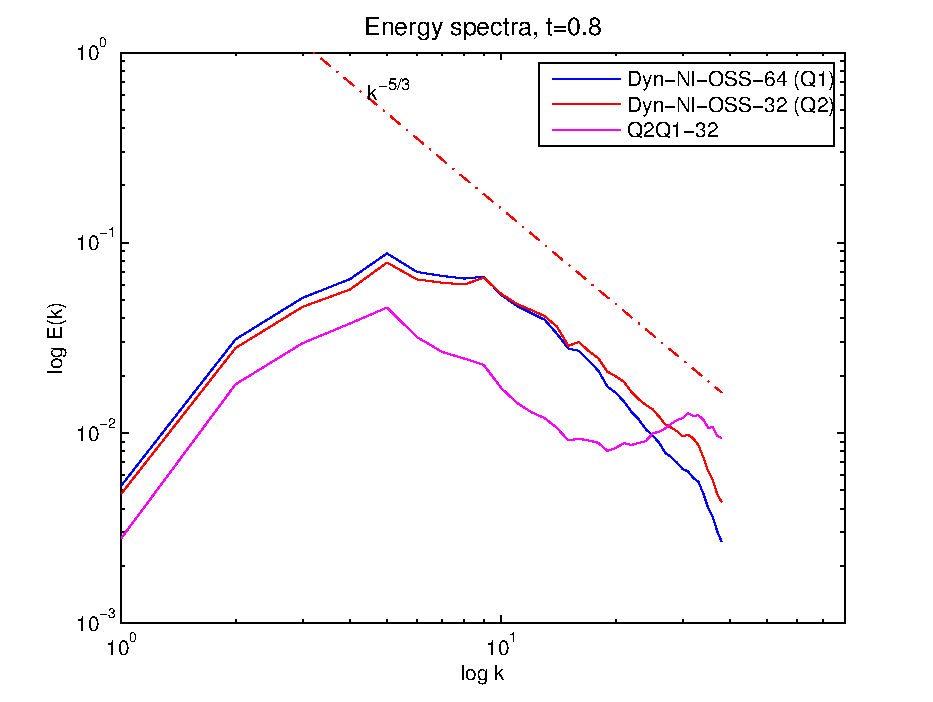
\includegraphics[width=0.49\textwidth]{Figures/Chapter4/DHIT/spec_q2q1_scaled_t08}}
   \caption{Total kinetic energy evolution and energy spectra using OSS and non-stabilized method with an inf-sup stable $Q_2/Q_1$ element}
   \label{fig:ene_spec_q2q1}
\end{figure}

\subsection{Taylor-Green Vortex}
\label{subsec-C4_TGV}
This problem aims to show, in a relatively simple flow, the basic turbulence decay mechanisms like the turbulent energy cascade, the production of small eddies and the enhancement of dissipation by the stretching of vortex lines. We refer to Section \ref{subsubsec-C3_TGV} for a deeper description of this problem.

The computational domain is the unit cube with periodical boundary conditions. The initial analytical condition is defined in the physical space (see, e.g., \cite{gassner_accuracy_2013}), and given by
\begin{align}
\label{eq-C4_ini_sol_TG}
&u_x=u_0\cos(x)\sin(y)\sin(z),\\\nonumber
&u_y=-u_0\sin(x)\cos(y)\sin(z),\\\nonumber
&u_z=0,\\\nonumber
&p=p_0+\frac{1}{16}\left(\cos(2x)+\cos(2y)\right)\left(\cos(2z)+2\right),
\end{align}
with
$$u_0=\frac{2}{\sqrt{3}}\sin\left(\gamma+\frac{2\pi}{3}\right).$$
We choose $\gamma=0$, which gives the mean initial velocity  $u_0=1$. The pressure constant parameter $p_0$ is chosen equal to zero.

\subsubsection{Setting}

We solve the TGV problem using a Reynolds number ${\rm Re}=1600$. 
The most common Reynolds numbers available in the literature are ${\rm Re}=800$, ${\rm Re}=1600$ and ${\rm Re}=3000$ (see, e.g., \cite{andrea_d._beck_numerical_2012, fauconnier_construction_2009, gassner_accuracy_2013, jb_chapelier_final_2012}).
We use the same VMS methods as for the DHIT problem defined in Section \ref{subsec-C4_DHIT} to solve this test, namely the ASGS and OSS methods, both with linear and nonlinear definitions of the convective term and static or dynamic tracking in time of the subscales, as it is summarized in Table \ref{table:DHIT_cases}.
The stabilization parameters for each method are the same as those chosen for the DHIT test, see Subsection~\ref{subsubsec-C4_DHIT_setting}, and discussed in Section \ref{subsec-C4_effect_const}.

Initially we consider a mesh of $32^3$ hexahedral linear elements $(Q_1)$, but we will redefine this discretization to analyze the method performance when we refine the mesh, decreasing the element size $h$ or increasing the degree of the interpolation polynomial $p$. It implies to solve the problem on meshes with $64^3$ and $128^3$ linear $(Q_1)$, quadratic $(Q_2)$ or cubic $(Q_3)$ hexahedral elements. We also use a $20^3(Q_3)$ discretization to compare against other authors results.

\subsubsection{Vorticity}
The TGV test is characterized by its laminar evolution at the initial time steps, when the flow is strongly anisotropic due to the structured large-scale vortices directly related to the initial condition. If the Reynolds number is large enough, the vortex-stretching process, which activates the energy cascade effect, transfers energy from large to small-scales and the flow becomes unstable and turbulent. According to Brachet \emph{et al.} \cite{brachet_small-scale_1983}, the flow becomes nearly isotropic for ${\rm Re}\geq1000$.

In Fig. \ref{fig:isovor_vel_TG} we present some vorticity isosurface images showing this process for  a $128^3$ linear hexahedral elements mesh, for the dynamic and nonlinear OSS method. Note that the initial condition (Fig. \ref{fig:isvor_vel_1}) consists in eight vortices with the same scale corresponding to the eight Fourier modes located at $\mathbf{k}=(\pm1,\pm1,\pm1)$, as it has been pointed out previously.
\begin{figure}[p]
  \centering
  \subfigure[Isosurface for $|\omega|=1.0$ at $t=0.0$]{\label{fig:isvor_vel_1}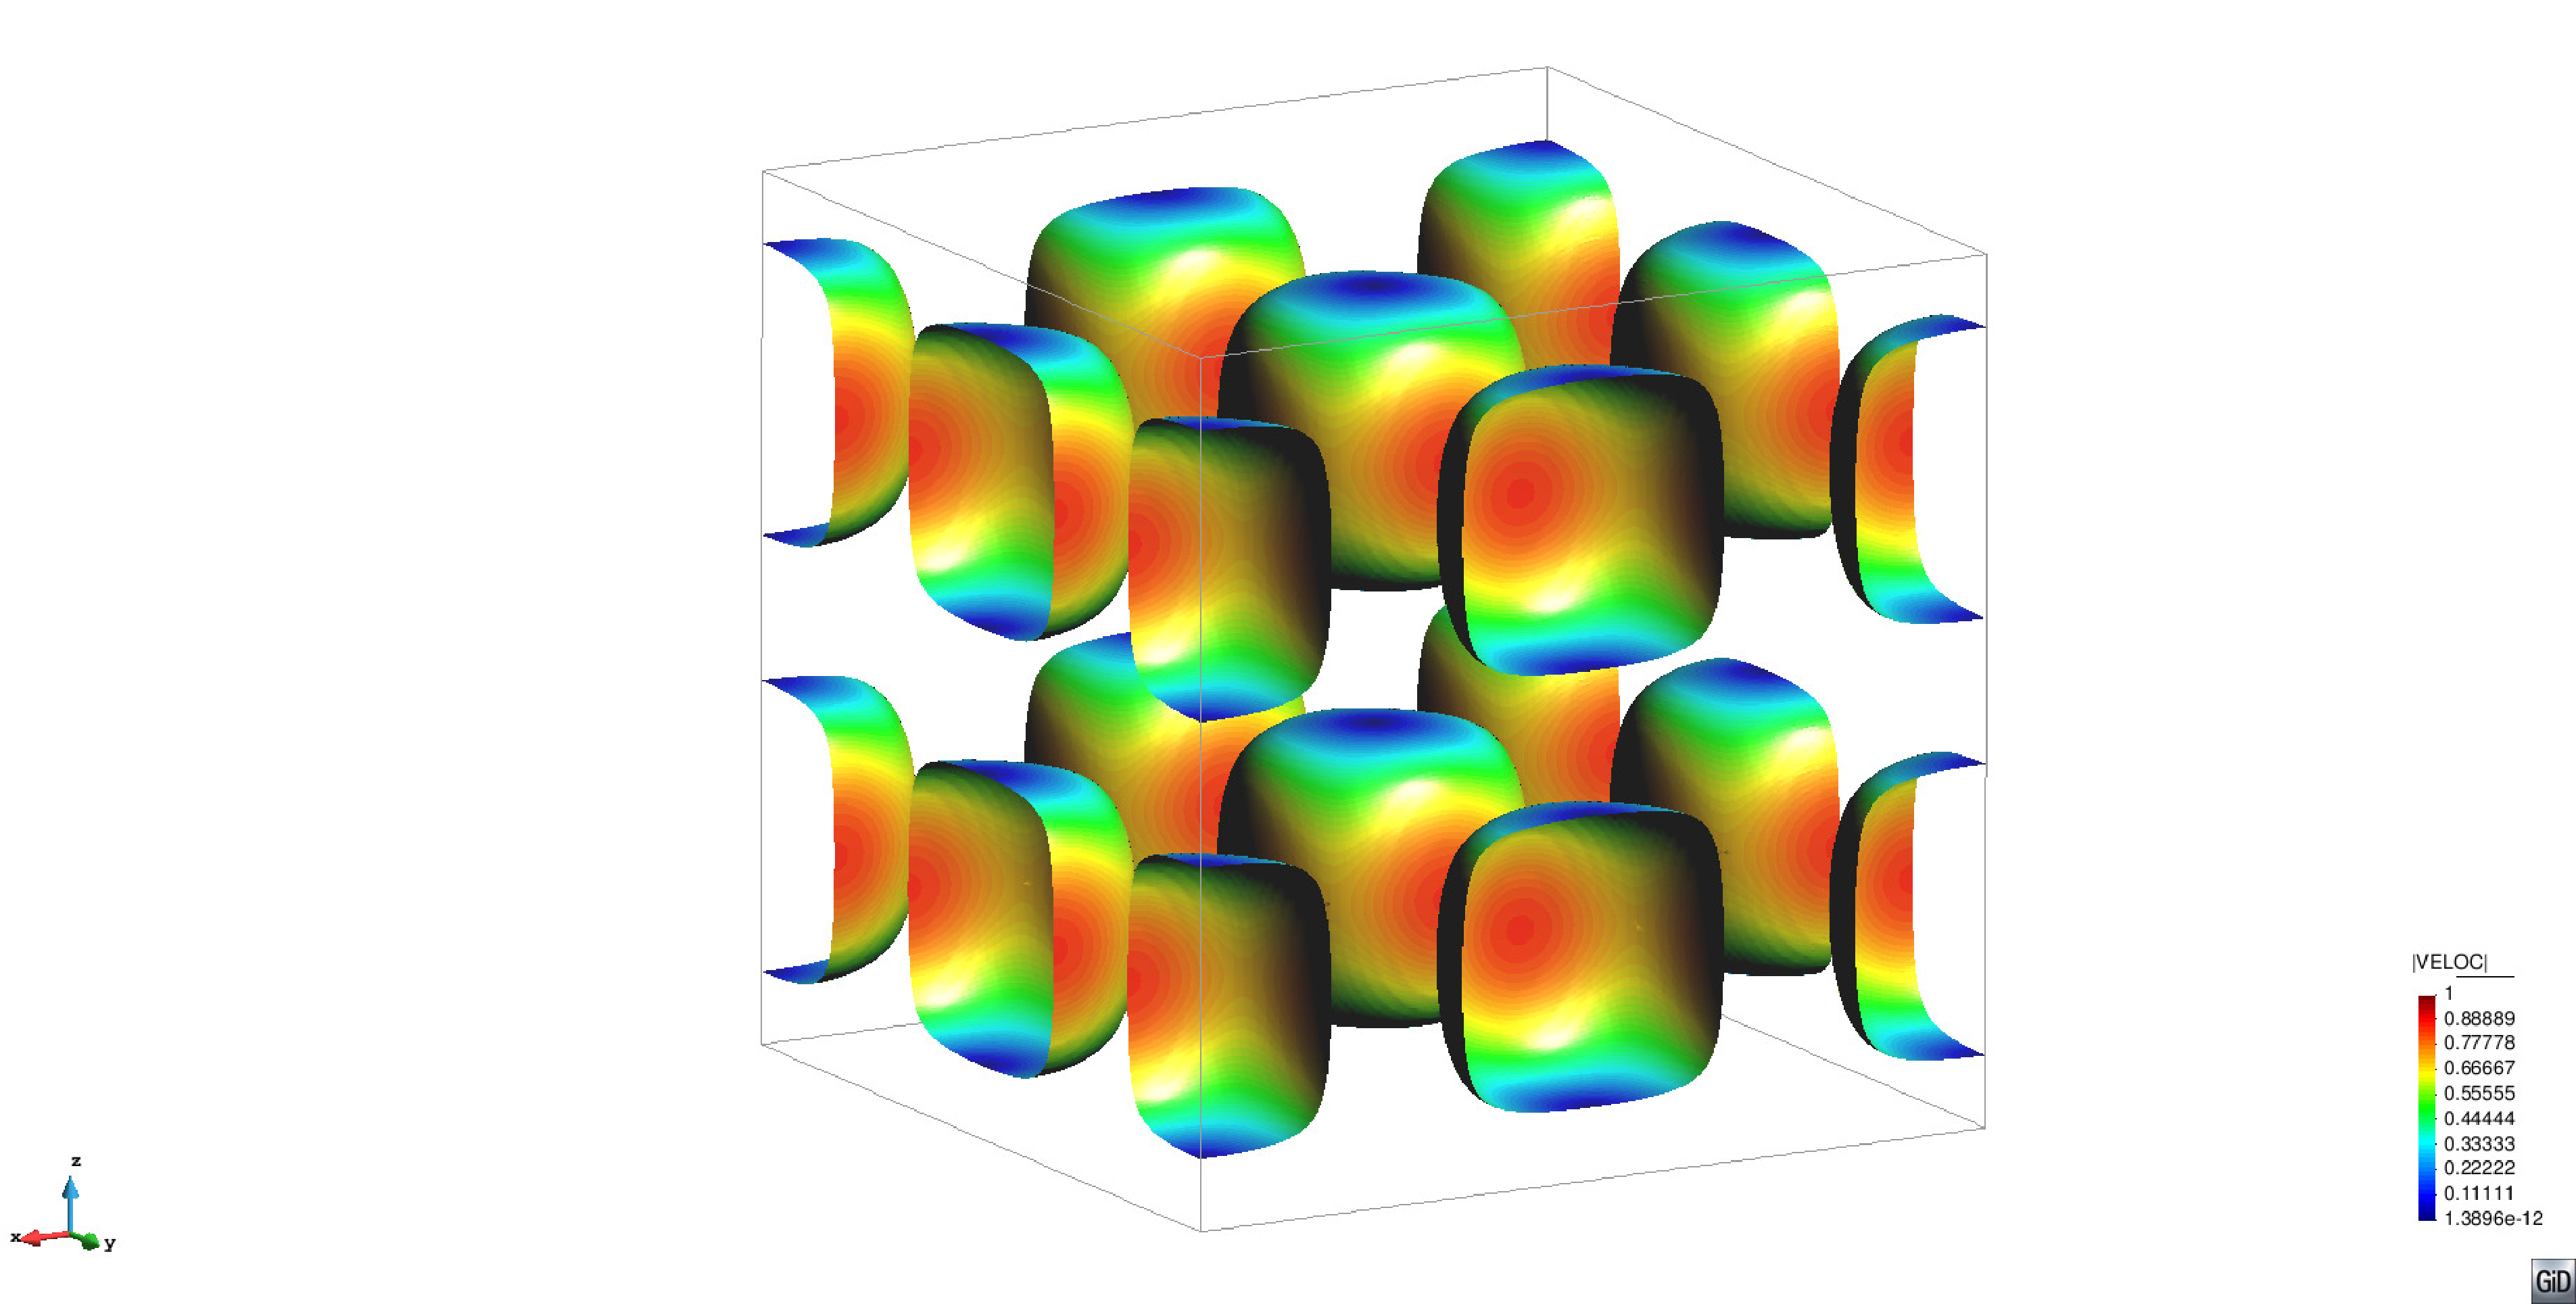
\includegraphics[clip=true, trim=13.5cm 0cm 13.5cm 0cm, width=0.49\textwidth]{Figures/Chapter4/TG/isovorti_veloc_1}}    
  \subfigure[Isosurface for $|\omega|=1.0$ at $t=2.0$]{\label{fig:isvor_vel_2}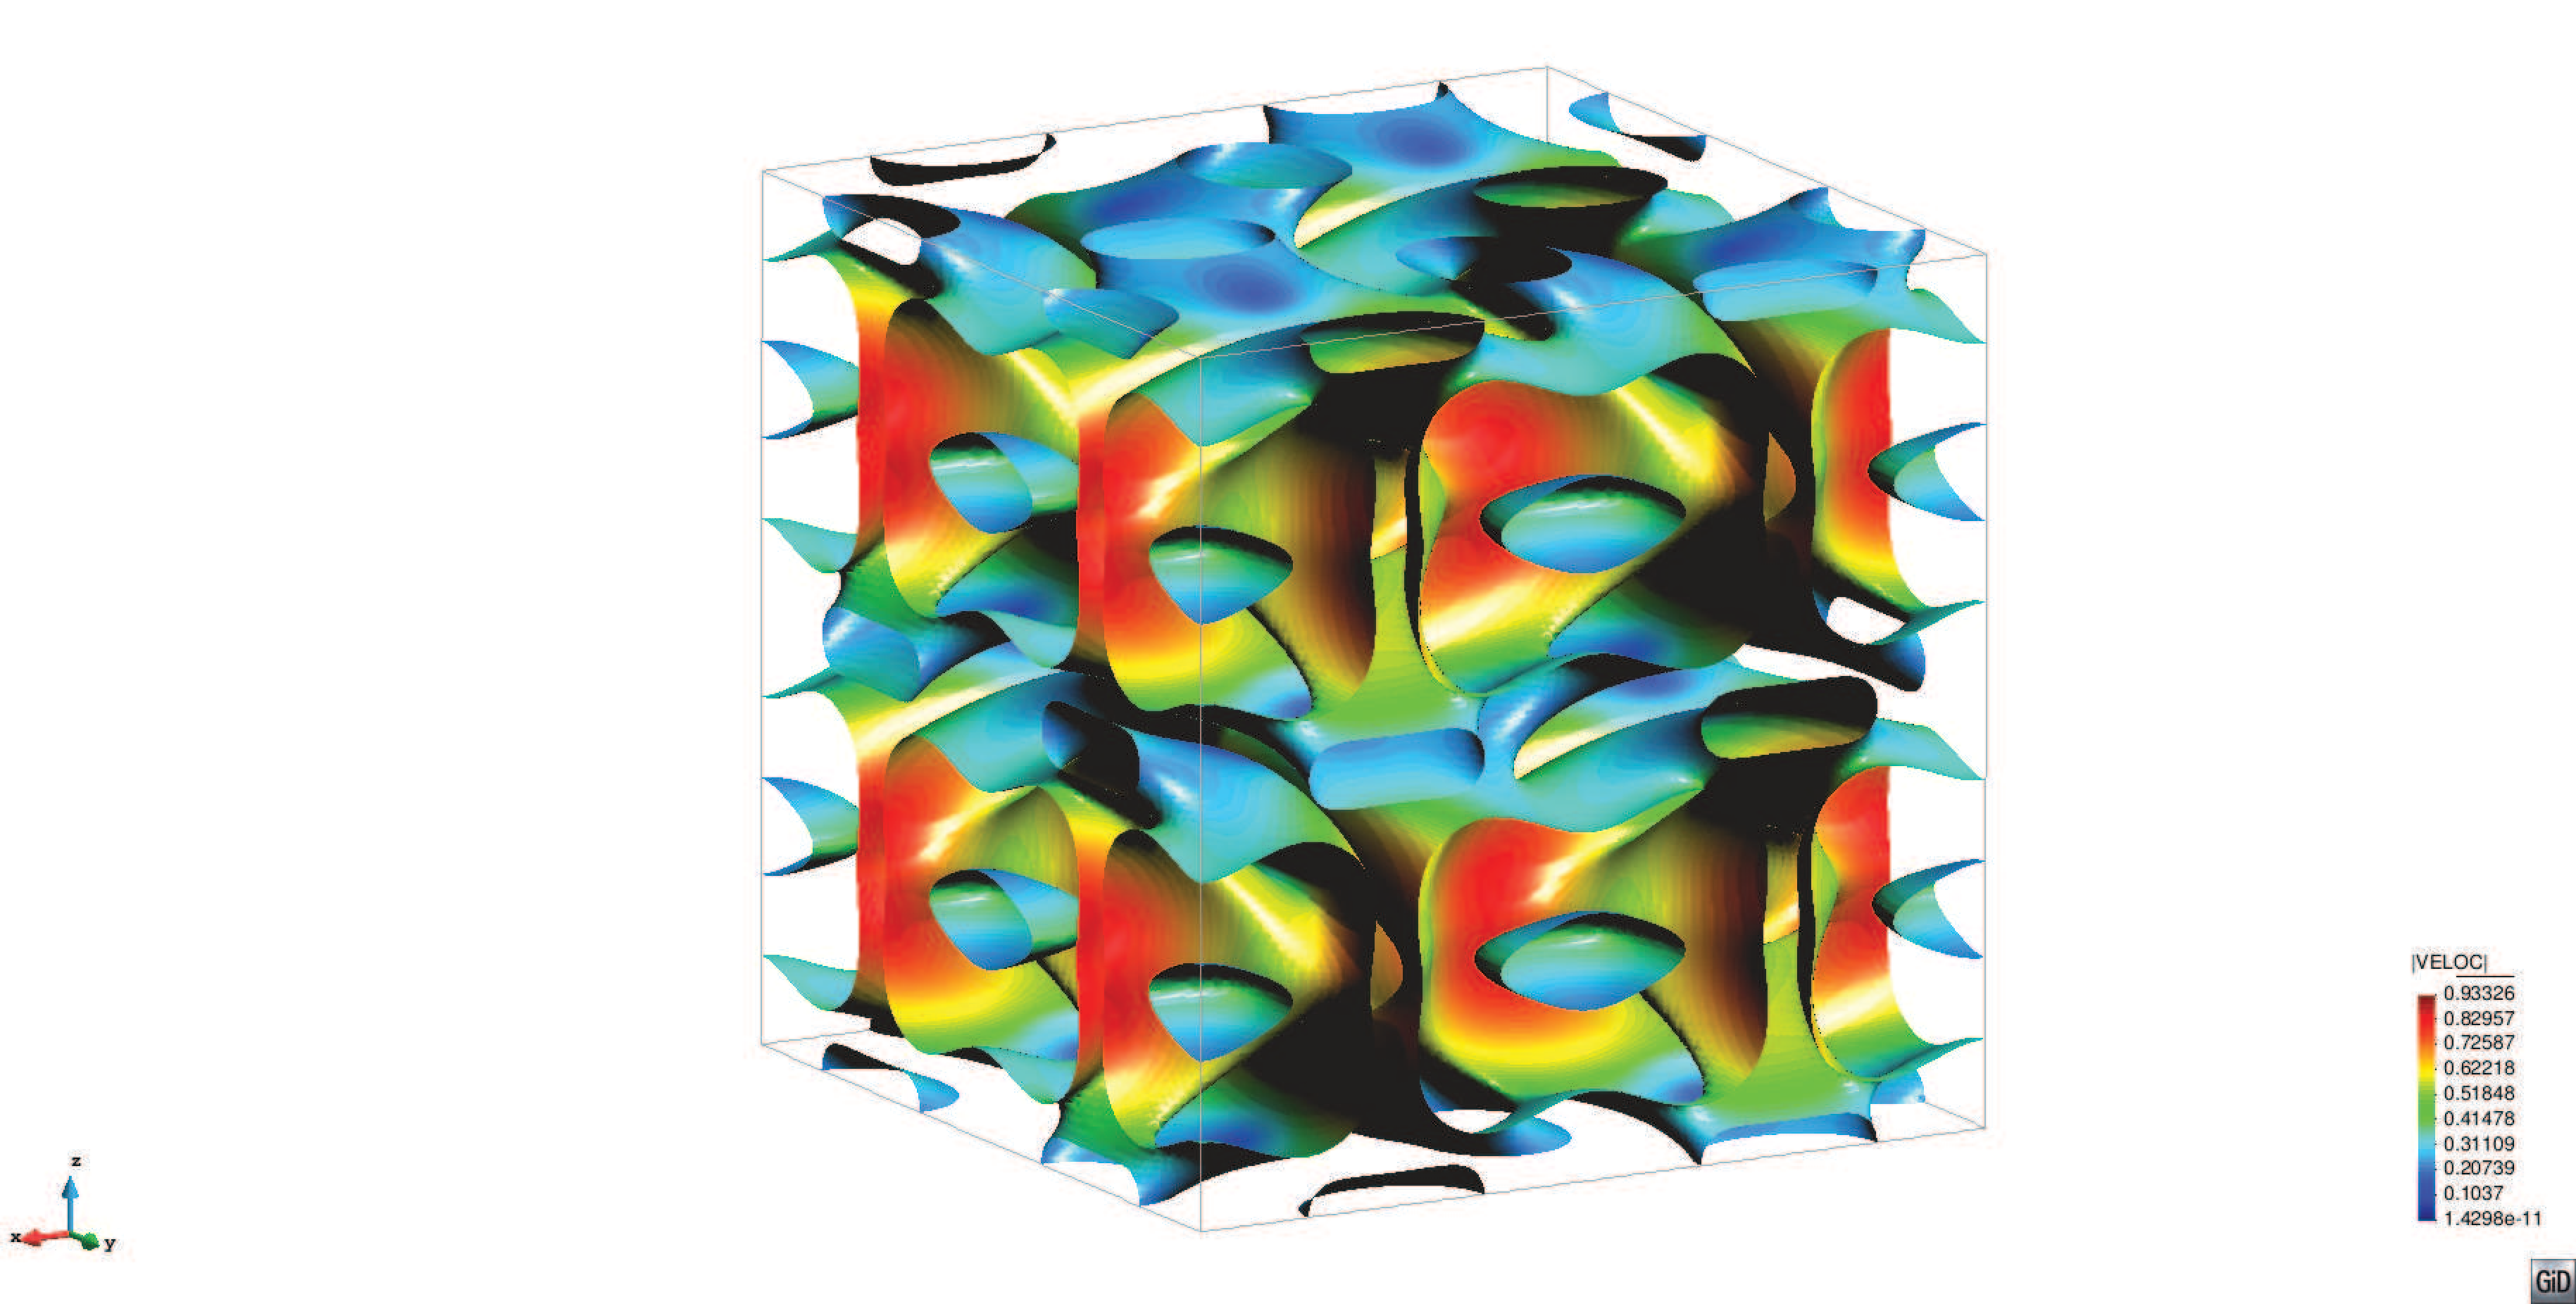
\includegraphics[clip=true, trim=13.5cm 0cm 13.5cm 0cm, width=0.49\textwidth]{Figures/Chapter4/TG/isovorti_veloc_2}}\\
    \centering
  \subfigure[Isosurface for $|\omega|=2.5$ at $t=4.1$]{\label{fig:isvor_vel_3}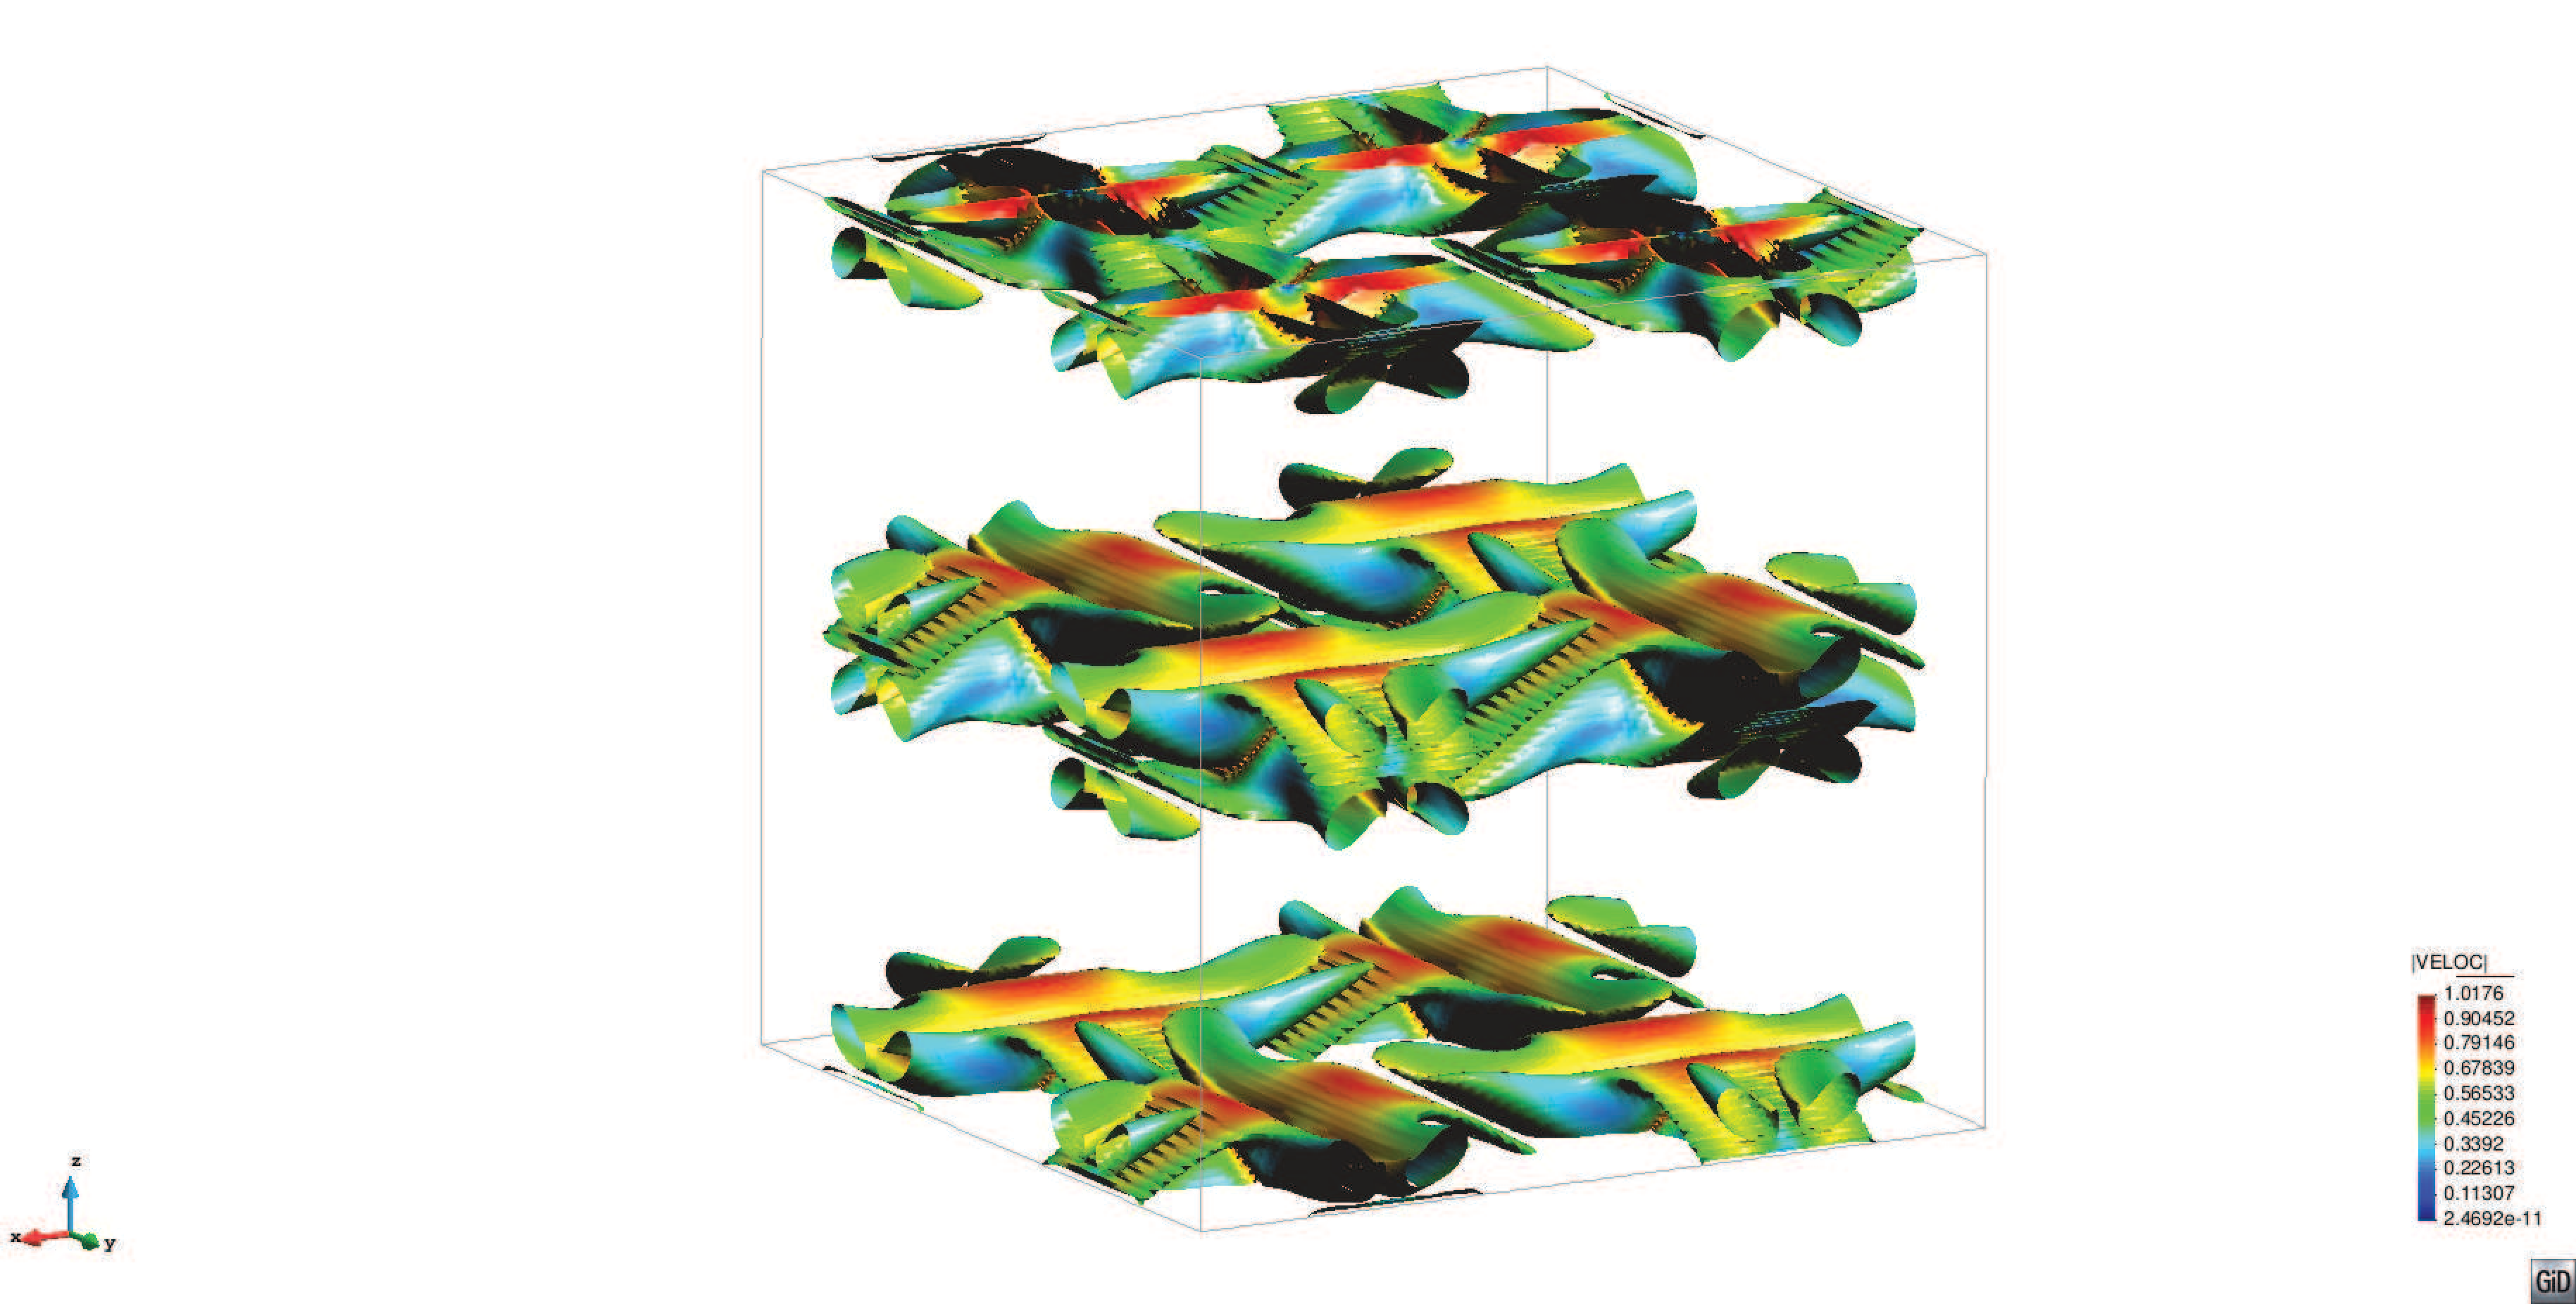
\includegraphics[clip=true, trim=13.5cm 0cm 13.5cm 0cm, width=0.49\textwidth]{Figures/Chapter4/TG/isovorti_veloc_3}}    
  \subfigure[Isosurface for $|\omega|=5.0$ at $t=6.1$]{\label{fig:isvor_vel_4}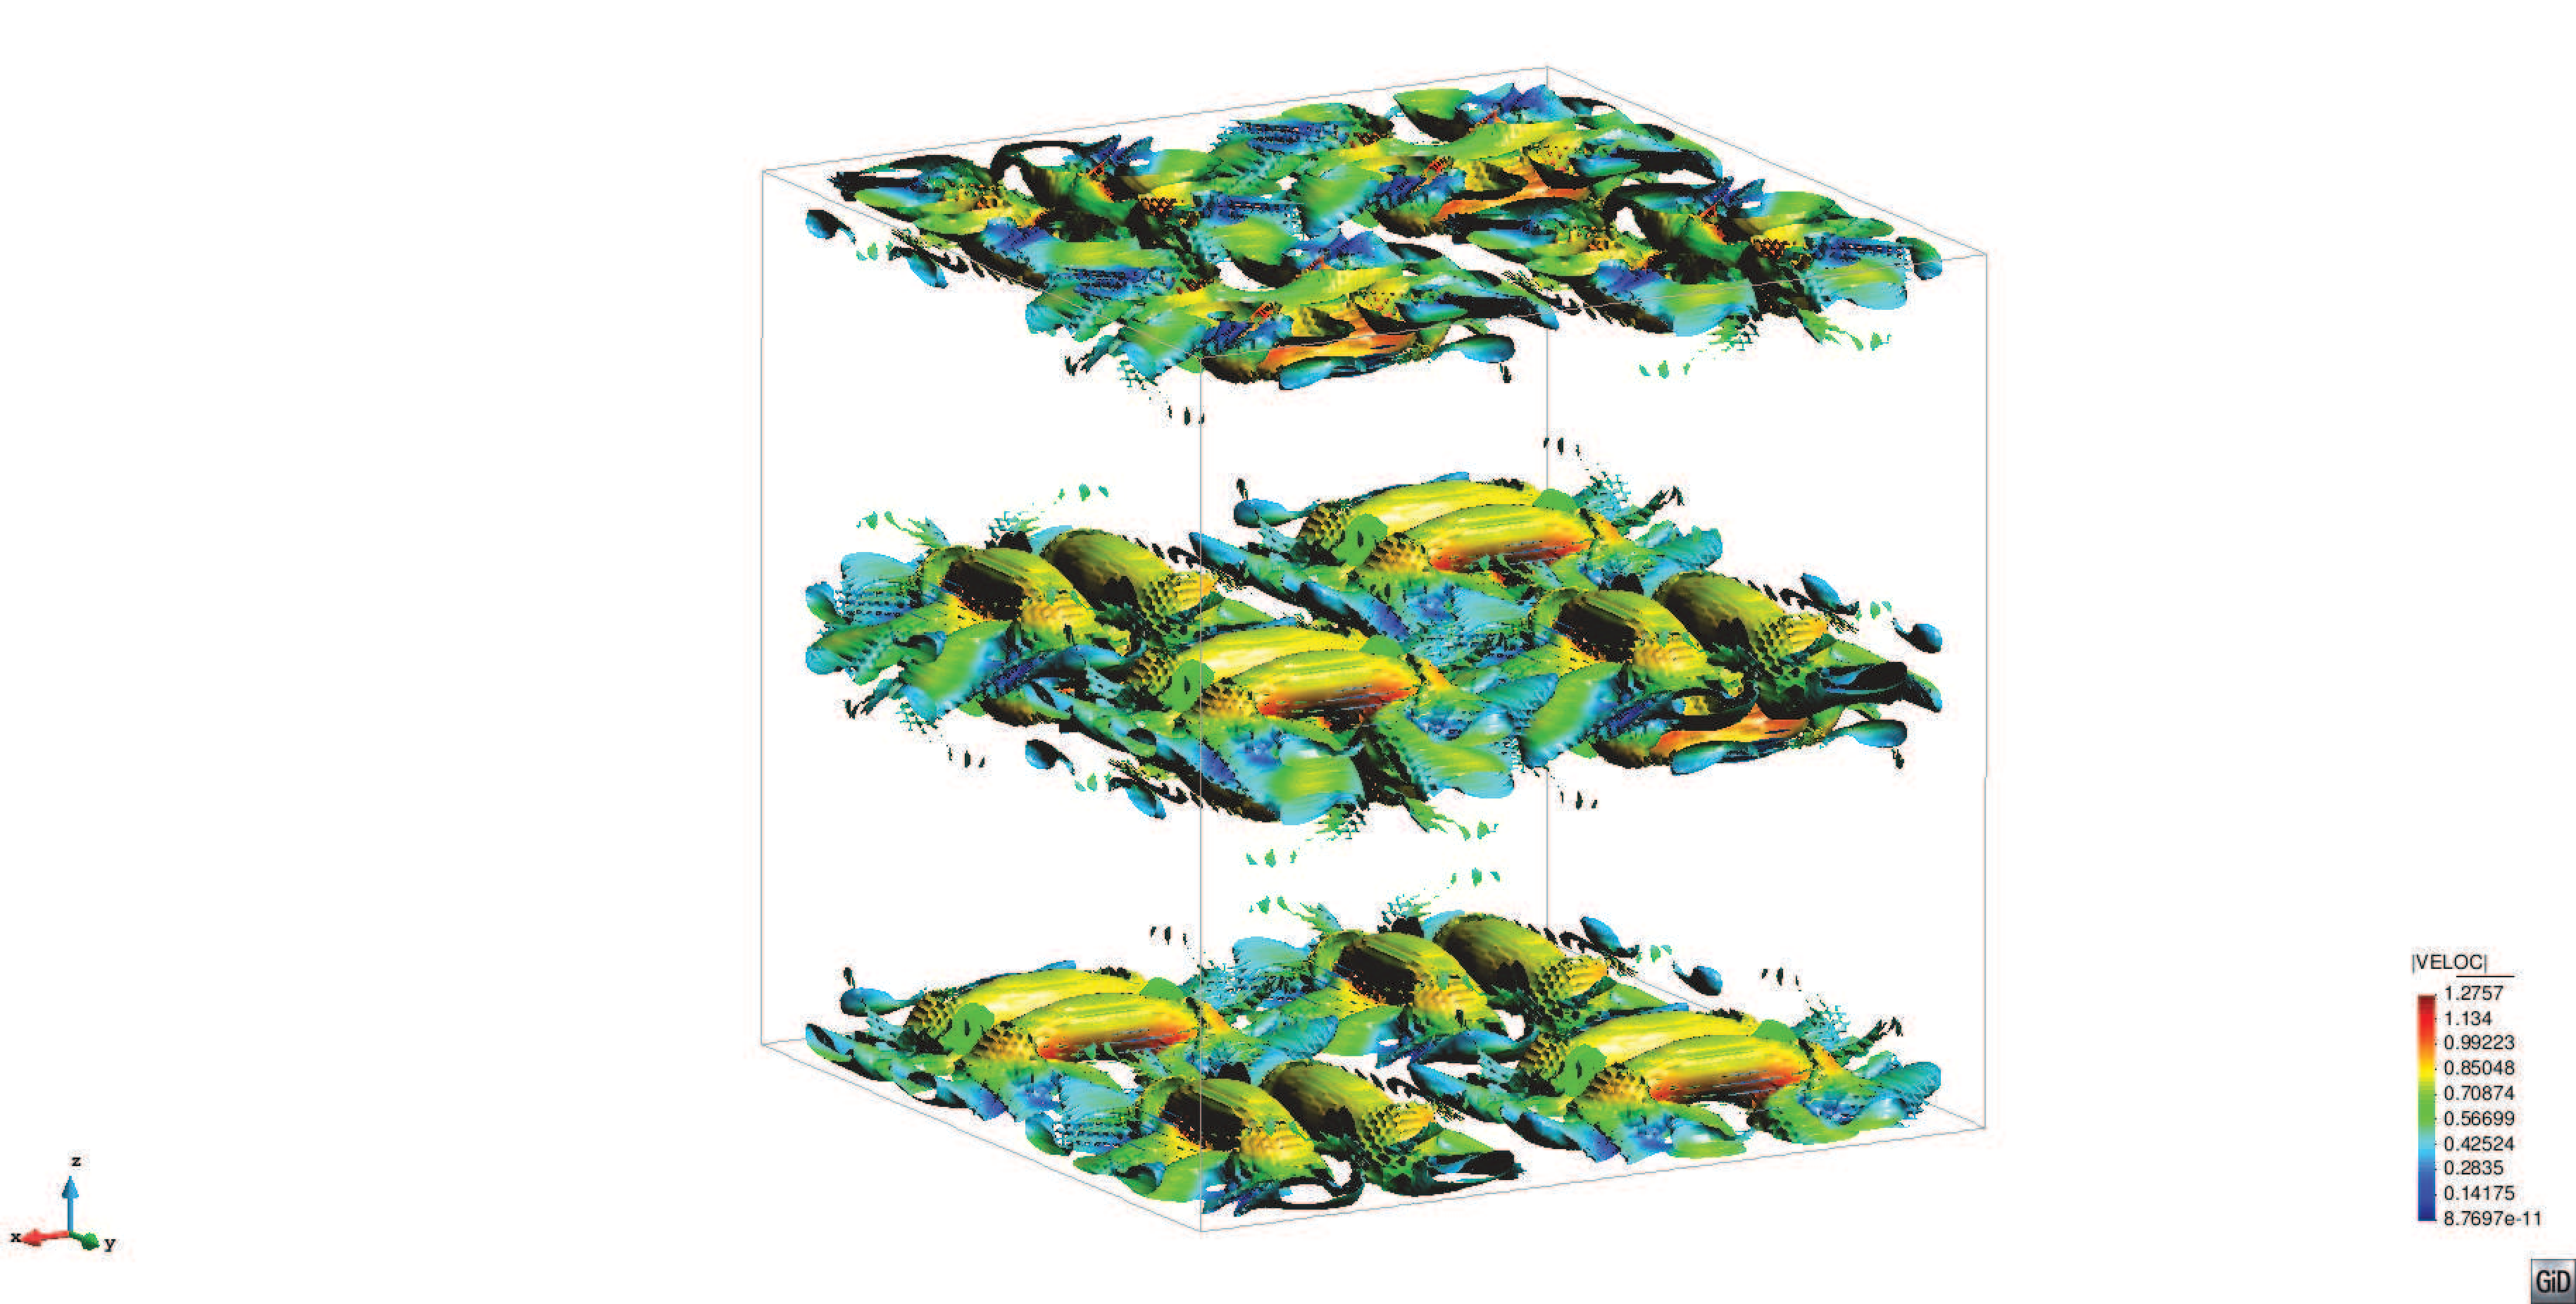
\includegraphics[clip=true, trim=13.5cm 0cm 13.5cm 0cm, width=0.49\textwidth]{Figures/Chapter4/TG/isovorti_veloc_4}}\\
    \centering
  \subfigure[Isosurface for $|\omega|=8.0$ at $t=8.2$]{\label{fig:isvor_vel_5}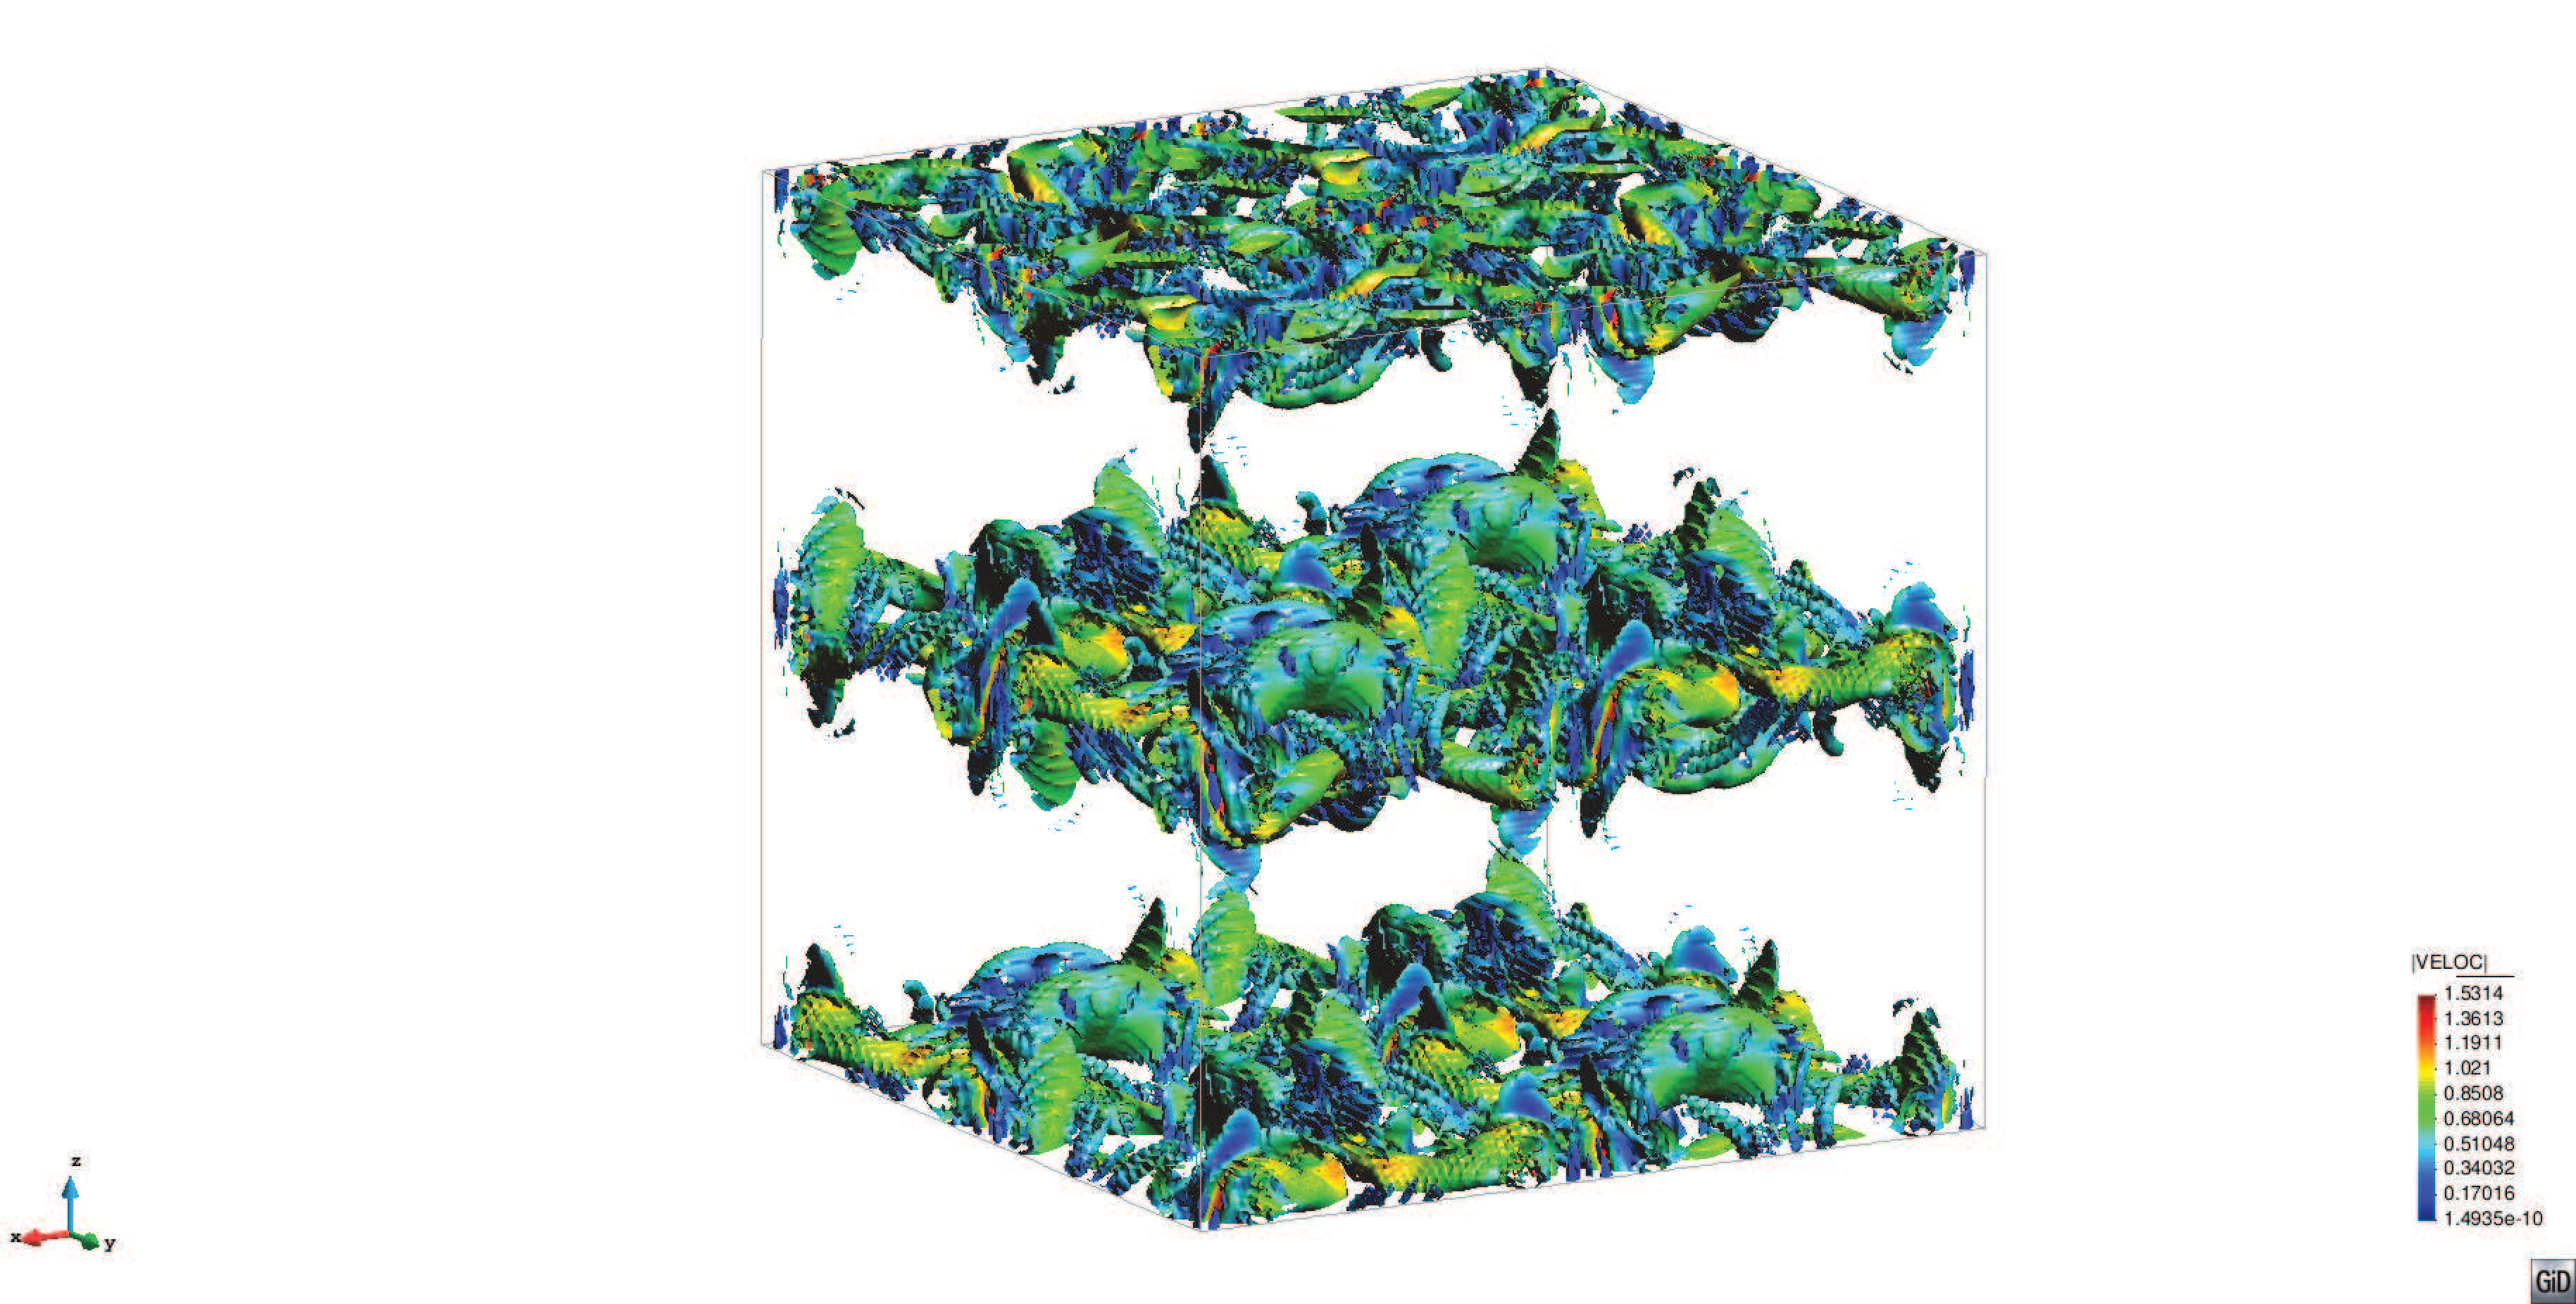
\includegraphics[clip=true, trim=13.5cm 0cm 13.5cm 0cm, width=0.49\textwidth]{Figures/Chapter4/TG/isovorti_veloc_5}}    
  \subfigure[Isosurface for $|\omega|=9.0$ at $t=10.2$]{\label{fig:isvor_vel_6}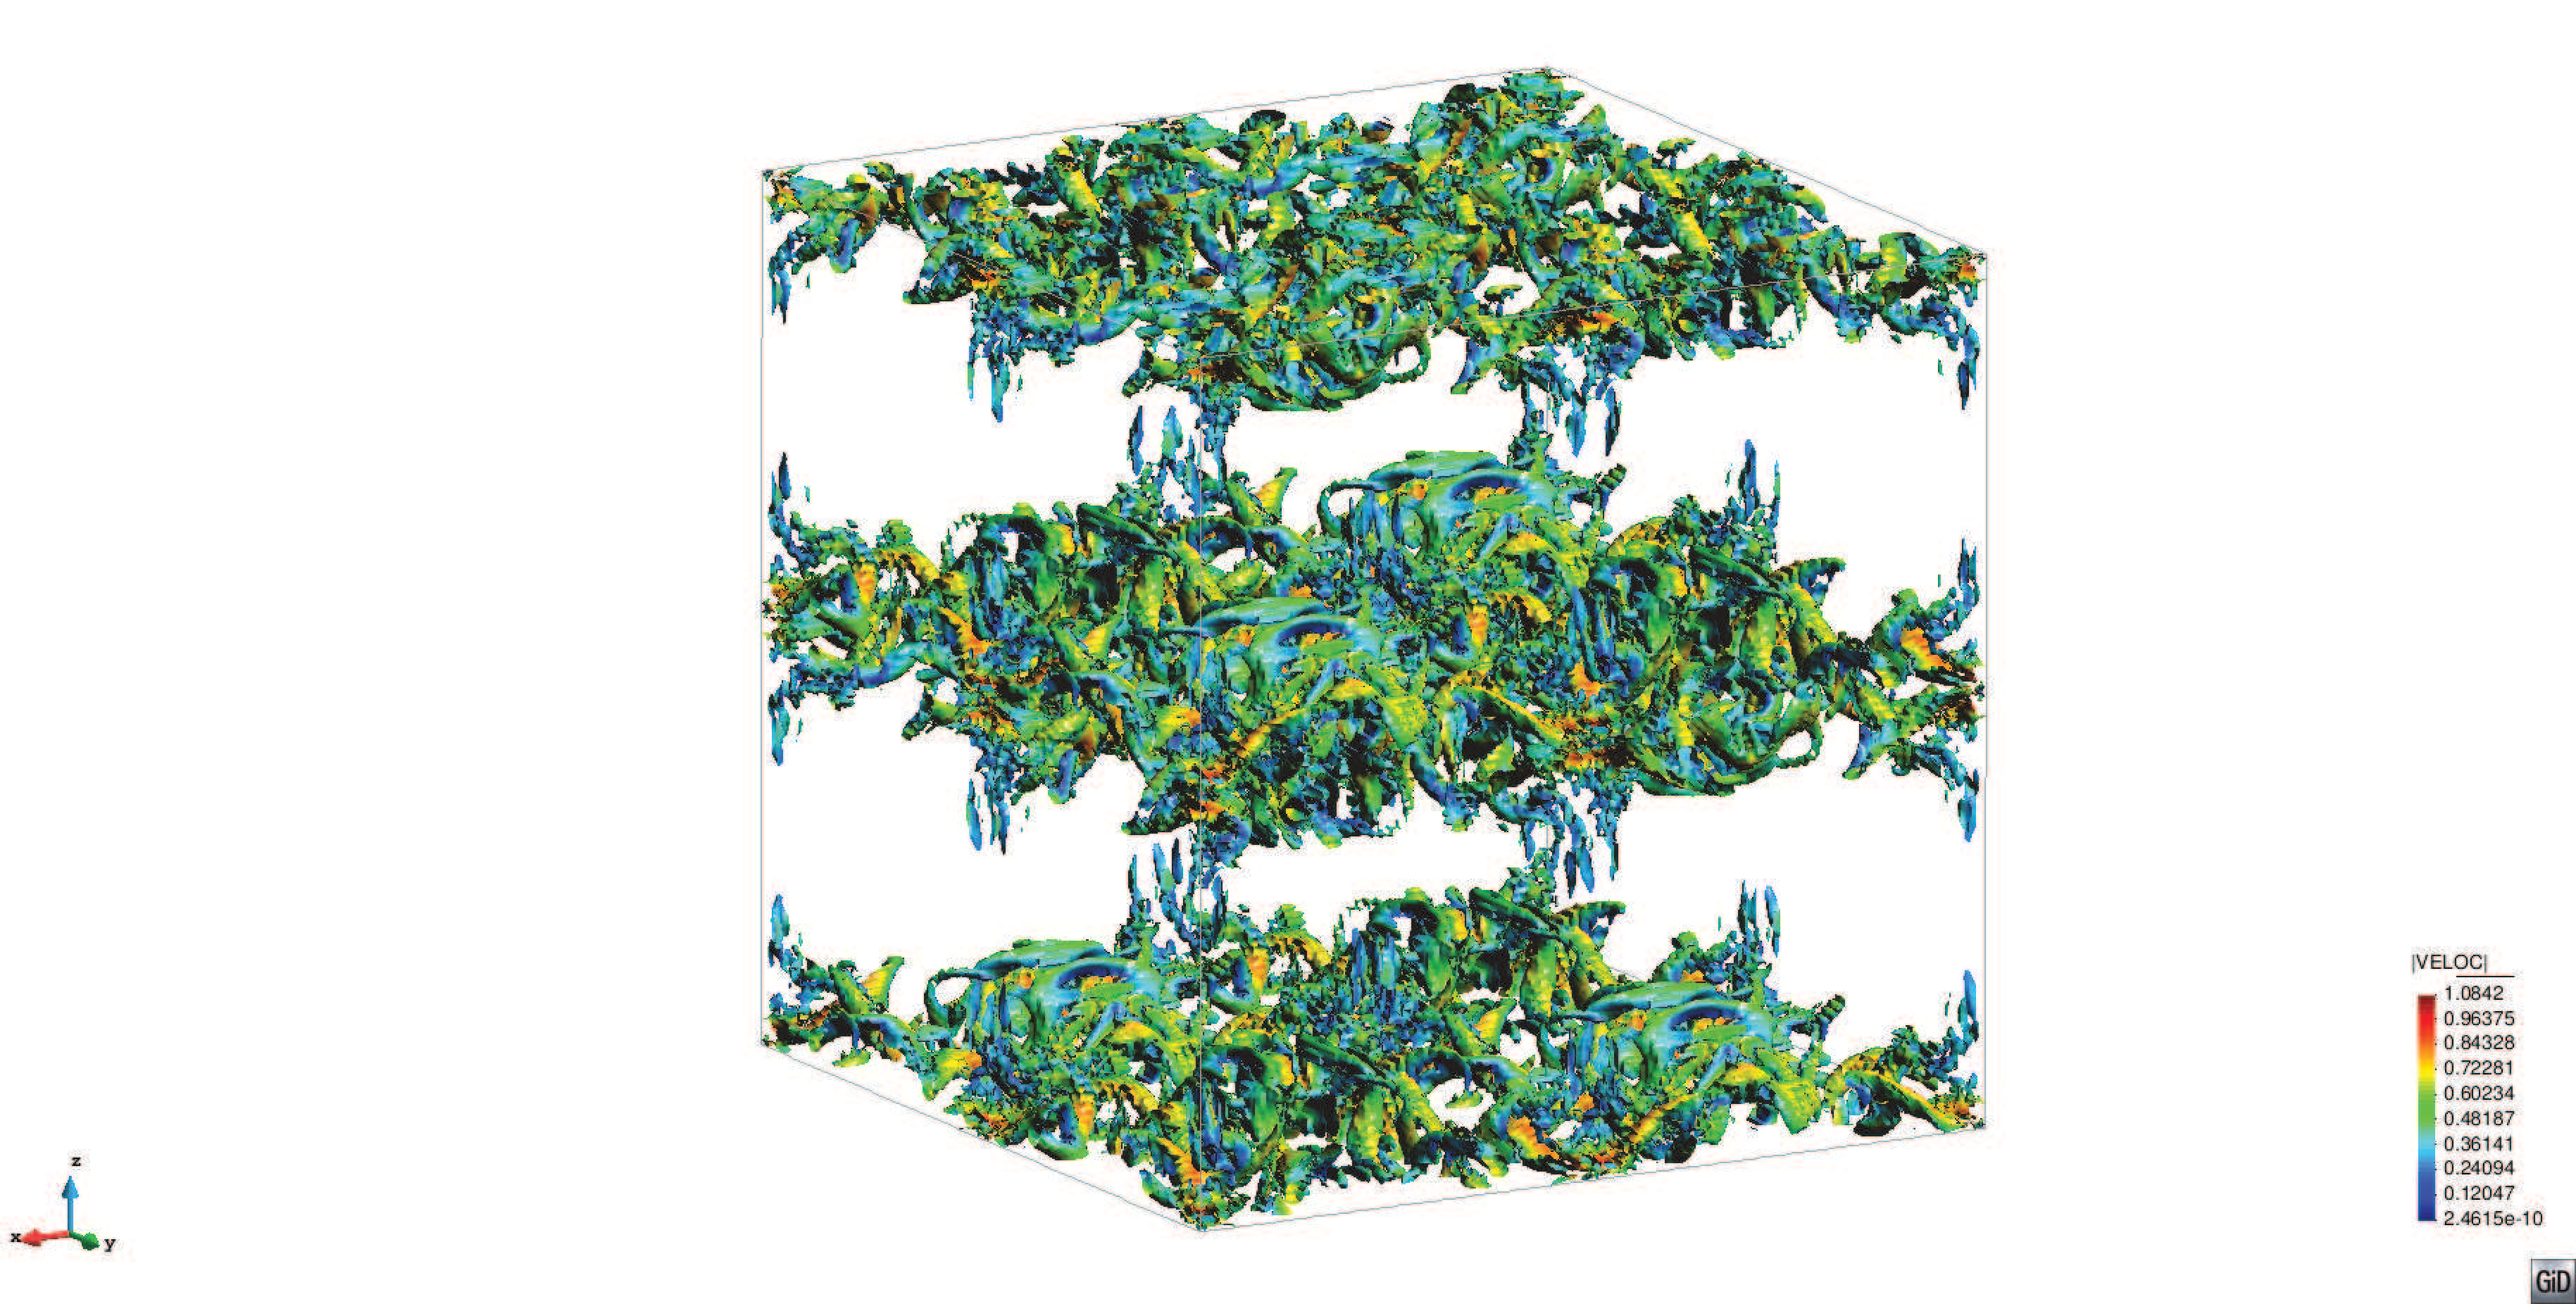
\includegraphics[clip=true, trim=13.5cm 0cm 13.5cm 0cm, width=0.49\textwidth]{Figures/Chapter4/TG/isovorti_veloc_6}}\\
  \caption{Vorticity isosurfaces with velocity contour at different time steps.}
  \label{fig:isovor_vel_TG}
\end{figure}

\subsubsection{Comparison between VMS methods}

In order to compare the different VMS methods defined previously and to test their performance as LES models
%see if they can be considered LES models, 
we solve the TGV test on a $32^3$ and $64^3$ linear elements mesh with a Reynolds number ${\rm Re}=1600$. 

We want to show the amount of numerical dissipation, the energy cascade in the spectra and the enstrophy evolution (compared to DNS) in all cases. We compare first the kinetic energy evolution  with the kinetic energy evolution obtained by Brachet \emph{et al.} \cite{brachet_small-scale_1983}, (Fig. \ref{fig:ene_32_TG}). We also present the energy spectra at $t=9$, when the flow is supposed to be nearly isotropic at large wave numbers, (Fig. \ref{fig:spec_32_TG}).
\begin{figure}[h!]
 	\centering	
 	\subfigure[Total kinetic energy evolution]{\label{fig:ene_32_TG}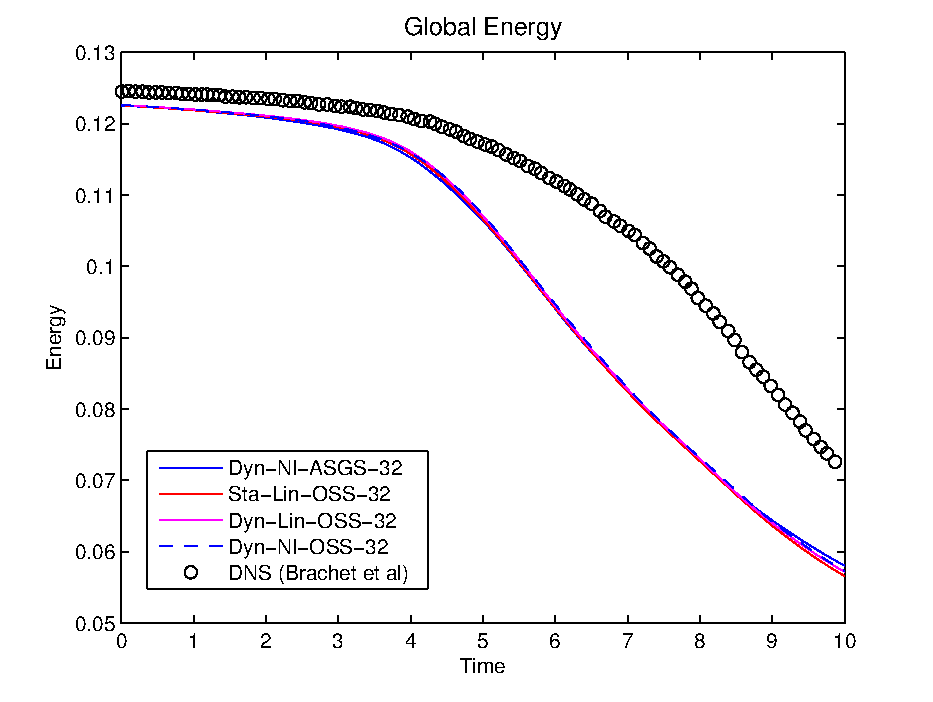
\includegraphics[width=0.49\textwidth]{Figures/Chapter4/TG/ene_32_new}}
 	\subfigure[Energy spectra at $t=9.0$]{\label{fig:spec_32_TG}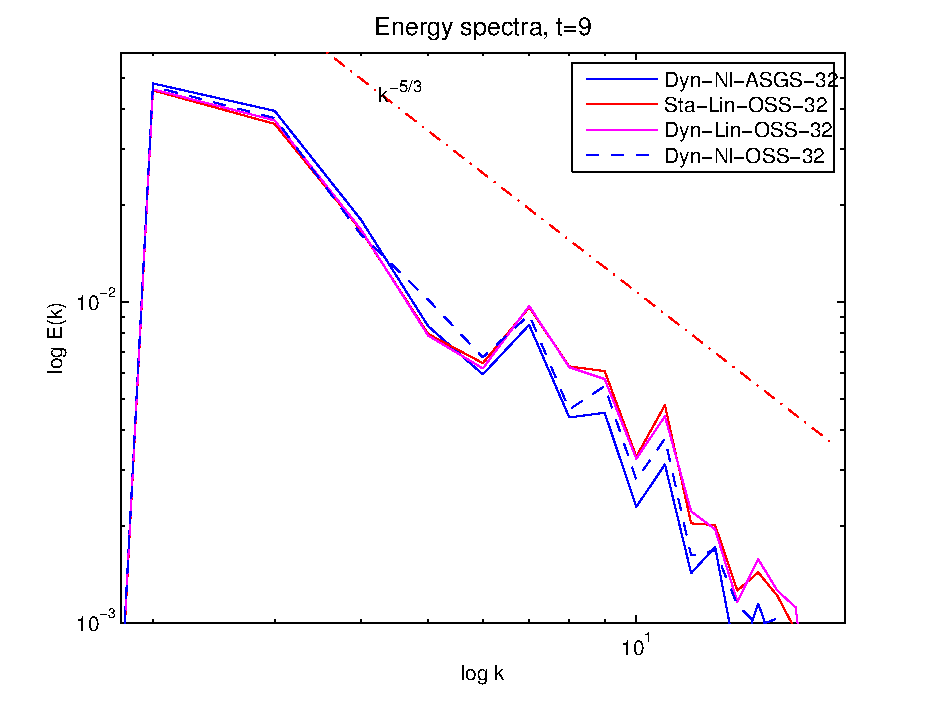
\includegraphics[width=0.49\textwidth]{Figures/Chapter4/TG/spec_32_x2_new}}
 	\caption{Total kinetic energy evolution and energy spectra}
 	\label{fig:ene_spec_32_TG}
 \end{figure}

In Fig. \ref{fig:ene_32_TG}, we can see that for a $32^3$ trilinear hexahedral elements mesh all methods show a premature decay of energy. We recognize the same behavior observed for the same mesh in the DHIT test, see Subsection \ref{subsubsec-C4_Total_ene_DHIT}. For this mesh, it is clear that the methods are not able to simulate properly the transition to turbulence. The energy spectra at $t=9.0$ shows us that the flow is isotropic at large wave numbers since it is decaying following the $k^{-5/3}$ Kolmogorov law. 

As in the DHIT test, the cases with nonlinear and dynamic definitions of the subscales, using either ASGS or OSS methods, seem to be slightly less dissipative. Furthermore, OSS is a little bit less dissipative than ASGS, but the differences are not important. 

As for the DHIT test, the results obtained using the different methods listed in Table \ref{table:DHIT_cases} are very similar for these coarser discretizations. The only point that is worth to note is that the linear and static ASGS case (Sta-Lin-ASGS) and the dynamic and linear ASGS case (Dyn-Lin-ASGS) diverge at some time step before $t=9$. Anyway, all the methods converge as $h\rightarrow0$ and the accuracy depends much more on the mesh size than on the choice of the method. In turn, similar trends for the computational cost analyzed in the previous section have been observed.

\subsubsection{$h$-$p$ refinement}

As in the DHIT problem, we perform a refinement study reducing $h$ and/or increasing $p$ using  Dyn-Nl-OSS. 
The global energy evolution and the energy spectra are shown in Fig. \ref{fig:ene_spec_hp_TG}. Fig. \ref{fig:ene_hp_TG} displays the total kinetic energy evolution compared with the DNS \cite{brachet_small-scale_1983}. The results show that all cases, excluding the $32^3$ and $64^3$ linear hexahedral mesh, follow almost perfectly the line defined by the DNS result points. On the other hand, Fig. \ref{fig:spec_hp_TG} displays the energy spectra at $t=9$, when the dissipation is maximum and the flow is evolving to turbulence. We compare the energy spectra obtained solving all the cases considered before with the DNS computed by \cite{gassner_accuracy_2013}, using the same Reynolds number (${\rm Re}=1600$) at the same time. 
\begin{figure}[h!]
	\centering
	\subfigure[Total kinetic energy evolution]{\label{fig:ene_hp_TG}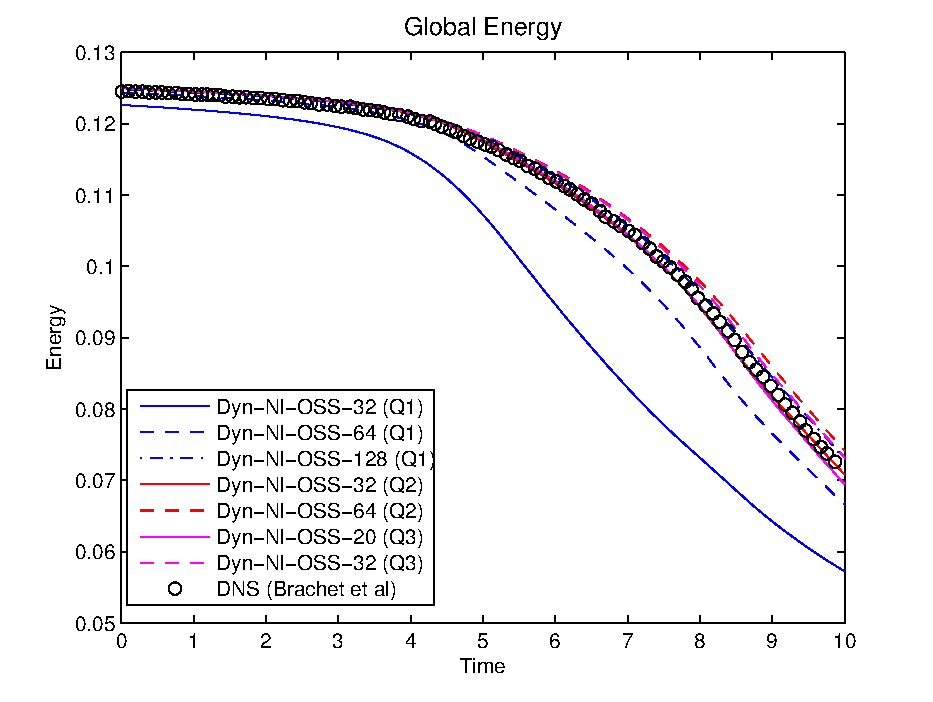
\includegraphics[width=0.49\textwidth]{Figures/Chapter4/TG/ene_hp_10_new}}
	\subfigure[Energy spectra at $t=9$]{\label{fig:spec_hp_TG}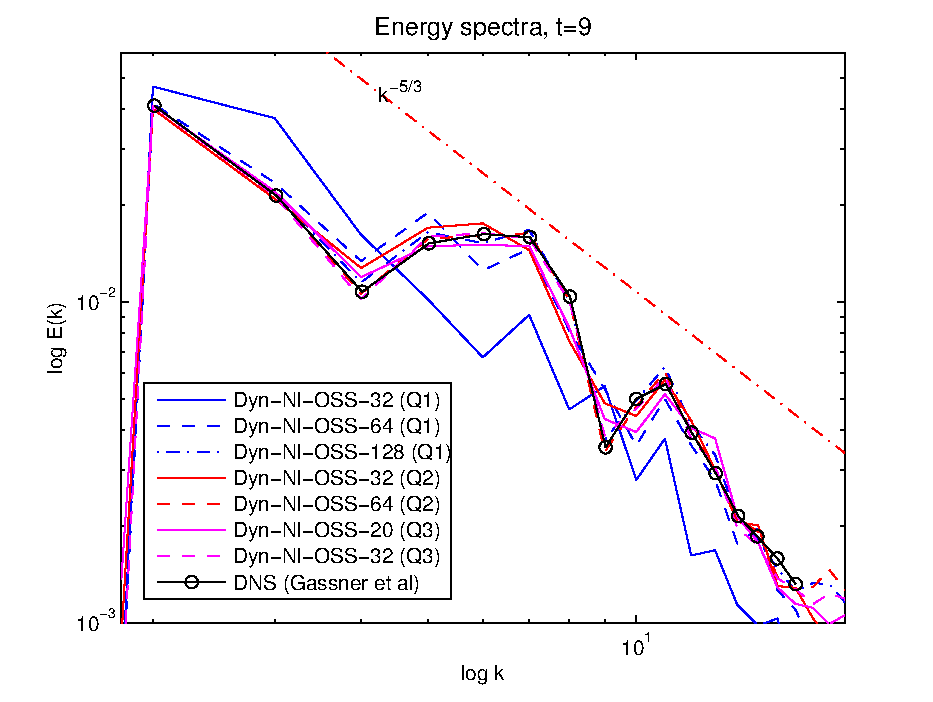
\includegraphics[width=0.49\textwidth]{Figures/Chapter4/TG/spec_hp_x2_new}}
	\caption{Total kinetic energy evolution and energy spectra for the $h-p$ refinement cases.}
	\label{fig:ene_spec_hp_TG}
\end{figure}

% Excluding the too coarse $32^3 (Q_1)$ approximation, the energy spectra follow accurately the DNS energy spectra. For low wave numbers, the differences with the DNS are minimal. It is on the highest wave numbers where some differences between the methods appear. Note that the $32^3(Q3)$ case follows very accurately the DNS spectrum. In general, we see that the spectra decay following a slope close to the $k^{-5/3}$ Kolmogorov law.
% %Anyway, we must emphasize that the flow is supposed to be isotropic after $t=9$, so we expect that this slope becomes closer to the predicted by Kolmogorov.

In Fig. \ref{fig:enediss_hp_TG} we show the dissipation rate of the problem, compared to the DNS results. The dissipation rate is directly related to the enstrophy of the problem, $\epsilon = 2\nu\left(\frac{1}{2}\left\langle|\omega|^2\right\rangle\right)$, where $|\omega|$ is the modulus of the vorticity. At the continuous level, it determines the kinetic energy decay which, at the discrete level, is also influenced by the numerical dissipation (see equation (\ref{eq-C4_FE_balance2})). When an explicit model is used, the dissipation introduced by the subgrid model also needs to be included. The FE viscous dissipation $\nu\|\nabla\u_h\|^2$, is shown in Fig. \ref{fig:enediss_hp_TG_resolved} whereas the total dissipation rate $ \nu\|\nabla\u_h\|^2 + \varepsilon_{h}$ defined by equation (\ref{eq-C4_FE_balance2}) is shown in Fig. \ref{fig:enediss_hp_TG_total}. 
%Fig. \ref{fig:ene_hp_TG} displays the total kinetic energy dissipation rate evolution for all the cases defined in Table \ref{table:refinement}, compared with the DNS \cite{brachet_small-scale_1983}. The results show that all cases, excluding the $32^3$ linear hexahedral mesh, follow almost perfectly the line defined by the DNS result points.
\begin{figure}[h!]
	\centering	
	\subfigure[Resolved]{\label{fig:enediss_hp_TG_resolved}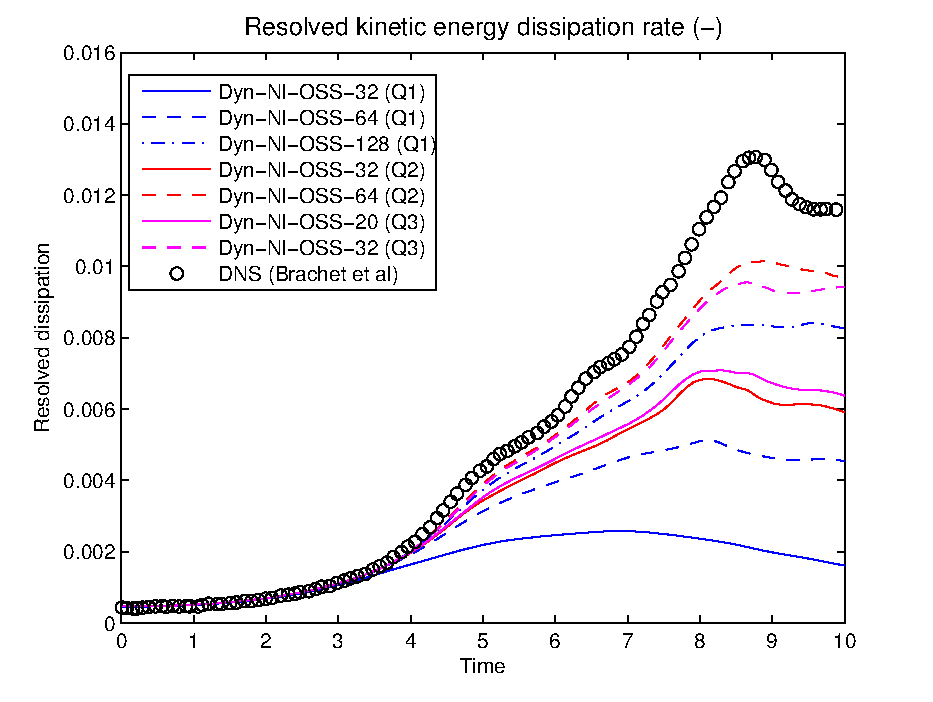
\includegraphics[width=0.49\textwidth]{Figures/Chapter4/TG/ens_hp_10_new_resolved}}
	\subfigure[Total]{\label{fig:enediss_hp_TG_total}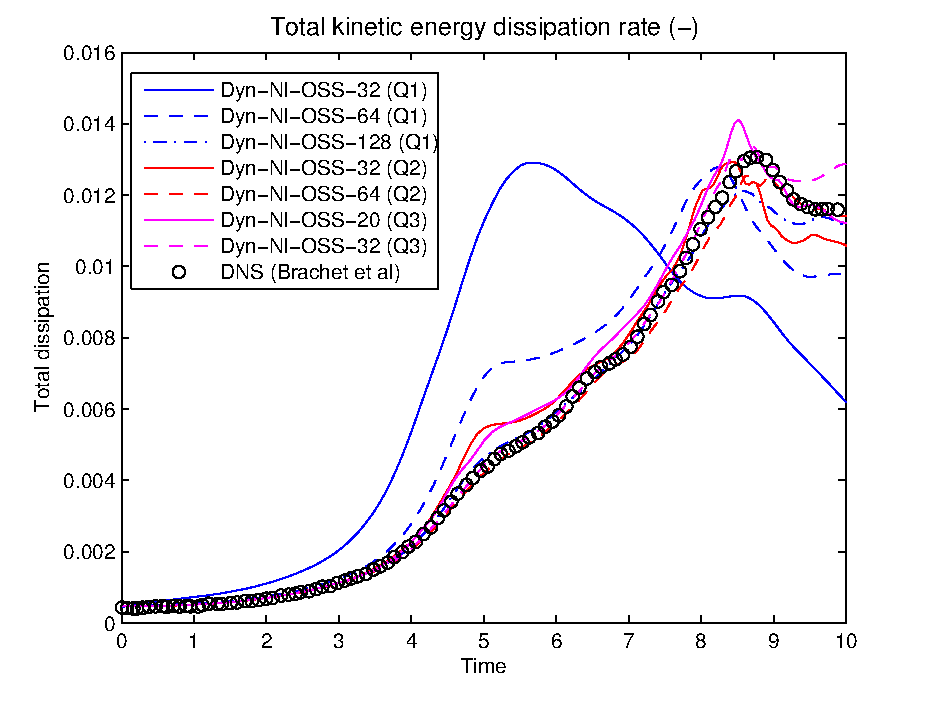
\includegraphics[width=0.49\textwidth]{Figures/Chapter4/TG/ens_hp_10_new_total}}
	\caption{Dissipation rate evolution for the $h$-$p$ refinement cases.}
	\label{fig:enediss_hp_TG}
\end{figure}

As in the DHIT problem, the results obtained using the coarser $32^3 (Q_1)$ and $64^3 (Q_1)$ meshes are not accurate, the FE viscous dissipation being far from the exact viscous dissipation, as shown in Fig. \ref{fig:enediss_hp_TG_resolved}. The total dissipation introduced by the method is too large and, especially for the $32^3 (Q_1)$, peaked at earlier times, i.e., the energy decays faster and earlier than it should (see Fig. \ref{fig:enediss_hp_TG_total}). When finer resolutions are used, the flows dynamics are much better predicted. Even when the resolution is not enough to completely capture the viscous dissipation, the total dissipation compares very well with the exact one, as shown in  Fig. \ref{fig:enediss_hp_TG}. This is a \emph{clear illustration of the very good performance of the method, which adds the right amount of dissipation when the gradients are not captured by the resolution.}

\subsubsection{Comparison with a non-stabilized method}

All the results presented up to this point have been computed using a VMS method, either ASGS or OSS. But, what would be the result using other methods? Are the methods presented here, comparable to classical LES methods? Which methods perform better? To answer all these questions, we compare the results obtained here against those obtained using the dynamic Smagorinsky model \cite{fauconnier_construction_2009} and the adaptive local deconvolution method \cite{hickel_adaptive_2006} specifically designed as an implicit LES model. The former has been obtained with a filter of size $2 \pi / 64$ and spectral resolution up to $2 \pi / 256$, thus not having numerical but only modeling error. In turn, the latter has been obtained using a $64^3$ grid without explicit subgrid model, an explicit third-order Runge-Kutta scheme for the time discretization, a fourth order spatial approximation of the symmetric terms and its particular approximation of the convective term which is based on the (forth order) five-point central stencils approximation of the convective term \cite{hickel_adaptive_2006}. To make the comparison as fair as possible we select those combinations of $h$ and $p$ that result in a similar number of degrees of freedom, which are $64^3 (Q_1)$ (second order), $32^3 (Q_2)$ (third order) and $20 (Q3)$ (fourth order) meshes (the last one having actually a bit less degrees of freedom).

The FE viscous dissipation is shown in Fig. \ref{fig:enediss_dynsmag_resolved} compared to the resolved dissipation obtained using the dynamic Smagorinsky model \cite{fauconnier_construction_2009} and the ``molecular dissipation'' of \cite{hickel_adaptive_2006} (the one computed using the molecular viscosity and the approximated solution, equivalent to our FE viscous dissipation but in the finite volume context). The total dissipations of the three methods are compared in Fig. \ref{fig:enediss_dynsmag_total}. 
\begin{figure}[h!]
	\centering	
	\subfigure[Resolved]{\label{fig:enediss_dynsmag_resolved}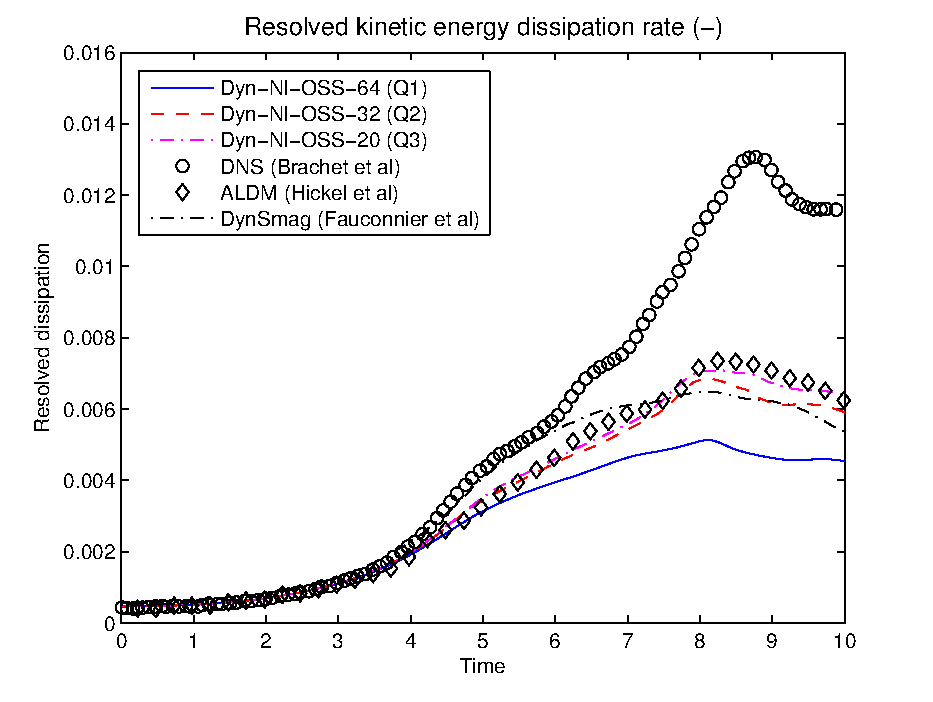
\includegraphics[width=0.49\textwidth]{Figures/Chapter4/TG/ens_64dofs_dynsmag_resolved}}
	\subfigure[Total]{\label{fig:enediss_dynsmag_total}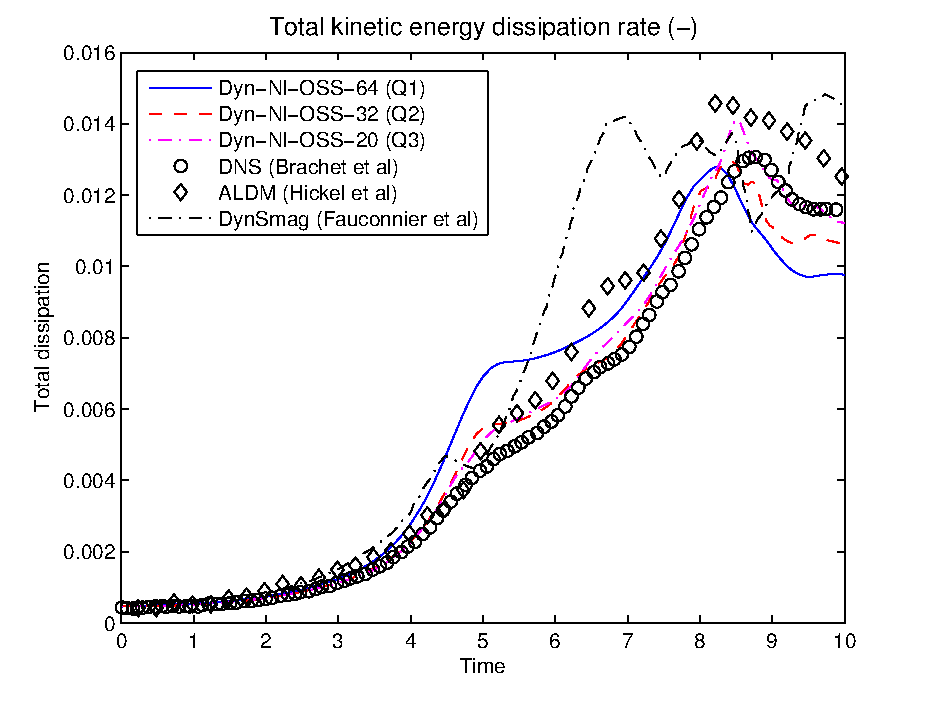
\includegraphics[width=0.49\textwidth]{Figures/Chapter4/TG/ens_64dofs_dynsmag_total}}
	\caption{Dissipation rate evolution compared to the dynamic Smagorinsky \cite{fauconnier_construction_2009} and ALDM models \cite{hickel_adaptive_2006}.}
	\label{fig:enediss_dynsmag}
\end{figure}

It can be observed in Fig. \ref{fig:enediss_dynsmag_resolved} that all the methods produce similar results, %. , ``certainly acceptable'' according to \cite{fauconnier_construction_2009} 
The dynamic Smagorinsky is more accurate in predicting the resolved dissipation at earlier times (up to $t\approx{}6$) but less accurate at later times (see Fig. \ref{fig:enediss_dynsmag_resolved}). 
%Nevertheless, 
We plot the total dissipation in Fig. \ref{fig:enediss_dynsmag_total}. We can see that the excellent job our implicit LES model does when the $20 (Q3)$ mesh is used, which would result in an excellent prediction of the resolved kinetic energy decay (which is not available in \cite{hickel_adaptive_2006}). 

\subsection{Turbulent channel flow}
\label{subsec-C4_TCF}
After studying the performance of VMS in the LES of homogeneous flows we turn our attention to wall-bounded turbulent flow and present results of fully developed turbulent flow in a channel.

This test consists of a fluid that flows between two parallel walls driven by an imposed pressure gradient which is defined by the Reynolds number based on the wall shear velocity, ${\rm Re}_\tau$. In the important amount of literature devoted to this problem, the usual Reynolds numbers are: ${\rm Re}_\tau=590$, ${\rm Re}_\tau=395$  and ${\rm Re}_\tau=180$ (see \cite{bazilevs_variational_2007, calderer_residual-based_2013, gamnitzer_time-dependent_2010, gravemeier_algebraic_2010, gullbrand_effect_2003, hughes_large_2001, john_variants_2008, kim_turbulence_1987, masud_variational_2011, moser_direct_1999}). We will restrict our attention to ${\rm Re}_\tau=180$ and ${\rm Re}_\tau=395$. See Section \ref{subsubsec-C3_TCF} for an extended description of this test.

\subsubsection{Setting}
\label{subsubsec-C4_TCF_setting}

We solve the problem using the coarsest mesh from previous tests, $32^3$ linear hexahedral $(Q_1)$ elements. The refinement in the wall-normal direction follows a hyperbolic function, also used in \cite{calderer_residual-based_2013,  gamnitzer_time-dependent_2010,  gravemeier_algebraic_2010, gullbrand_effect_2003, masud_variational_2011}, defined as 
$$y_i=\frac{\tanh\left(\gamma\left(\frac{2i}{np_y}-1\right)\right)}{\tanh(\gamma)},$$
where $i=1,...,np_y$ with $np_y$ the total amount of nodes in the wall-normal direction. Here, $\gamma$ is  chosen to be equal to $2.75$ for both  ${\rm Re}_\tau=180$ and ${\rm Re}_\tau=395$.  We refer the reader to \cite{avila_large_2014} for a complete study of the influence of the discretization in the results of the TCF.

As it has been said above, we solve the problem using two different friction Reynolds numbers, ${\rm Re}_\tau=180$ and ${\rm Re}_\tau=395$. We compare our results against those obtained by DNS in \cite{moser_direct_1999,kim_turbulence_1987} and we choose our parameters accordingly.
We take the bulk mean velocity and the half channel height equal to one, $\bar{U}=1$ and $\delta=1$. The viscosity is computed from the estimated Reynolds number based on the bulk mean velocity ${\rm Re}$. Then, from the friction Reynolds number ${\rm Re}_\tau$ we compute the friction velocity ($u_\tau$), the wall shear stress ($\tau_w$) and a driving force equivalent to a pressure gradient ($f_x$), given by  \cite{pope_turbulent_2000}:
$$u_\tau=\frac{\nu {\rm Re}_\tau}{\delta},\quad\quad\tau_w=\rho u_\tau^2,\quad\quad
f_x=\frac{\tau_w}{\delta}.$$

We use the Crank-Nicolson time integration scheme with a constant time step. Ham \emph{et al.}  test in \cite{ham_fully_2002} the influence of the time step for a fully implicit Finite Difference midpoint method, equivalent to Crank-Nicolson, on the statistics of a TCF DNS. They found little variation in statistical turbulence quantities up to $\delta t^+=1.6$. Following Gravemeier \emph{et al.} \cite{gravemeier_algebraic_2010}, we define a time step in wall units $\delta t^+=\frac{\delta tu_\tau^2}{\nu}\approx0.69$, which, according to \cite{ham_fully_2002}, should not affect the turbulent quantity statistics. The same authors performed 25000 time steps in order to allow the flow to develop and they collected the statistics during another 5000 time steps. A total averaging time about $500\delta/U_0$ is used in \cite{choi_effects_1994} once the statistically stable regime is achieved.

In Table~\ref{table:Channel_parameters} we present the value of the different parameters defined above for the two different friction Reynolds numbers. For the initial condition we impose a parabolic profile obtained solving the stationary Stokes problem with the driving force and viscosity defined above. Additionally, with the aim to achieve a fully developed flow earlier, we introduce a perturbation with a maximum value of $10\%$ the bulk velocity.

\begin{table}[h!]
\centering
\begin{tabular}{ccc}
\toprule
${\rm Re}_\tau$&$180$&$395$\\
\midrule
\midrule
$\nu$&$3.5714\cdot10^{-4}$&$1.4545\cdot10^{-4}$\\
$u_\tau$&$6.4286\cdot10^{-2}$&$5.7455\cdot10^{-2}$\\
$\tau_w$&$4.1327\cdot10^{-3}$&$3.3010\cdot10^{-3}$\\
$f_x$&$4.1327\cdot10^{-3}$&$3.3010\cdot10^{-3}$\\
$\delta t$&$0.06$&$0.03$\\
\bottomrule
\end{tabular}
\caption{Test parameters for the different friction Reynolds number.}
\label{table:Channel_parameters}
\end{table}

Our purpose is to check the VMS methods defined in Subsection \ref{subsec-C4_VMS_framework} for a wall-bounded flow. Following the computations performed for the previous tests, we solve the problem using the same cases defined in Table \ref{table:DHIT_cases} and the numerical parameters $\tau_c=0$ and $\tau_m$ are defined in the same way, now with the algorithmic constants  $c_1=12$ and $c_2=8$ (see Subsection \ref{subsec-C4_effect_const}) and the characteristic length, $h$, is chosen to be the minimum element length. 
%However, in the definition of the stabilization parameters (\ref{eq-C4_tau_m})-(\ref{eq-C4_tau_c}), the characteristic length, $h$, is choosen to be the minumum element length.

\subsubsection{Velocity profiles}
We first present the mean stream-wise velocity profile scaled by the wall shear stress velocity, $\langle u\rangle^+=\frac{\langle u\rangle}{u_\tau}$ for all cases defined in Table \ref{table:DHIT_cases}, where $\langle\cdot\rangle$  denotes the mean value in stream-wise and span-wise direction and in time, as a function of $y^+ = \frac{y u_\tau}{\nu}$.

In Fig. \ref{fig:Channel_umean_32} we show the mean stream-wise velocity normalized by the wall-shear velocity, $u_\tau$, obtained for all cases considered in Table \ref{table:DHIT_cases} in a $32^3$ linear elements mesh for the ${\rm Re}_\tau=395$ case. We compare the results with the DNS one obtained in  \cite{moser_direct_1999}. We can observe in Fig. \ref{fig:Channel_umean_32} that all methods perform quite similar and are very close to the DNS result. Fig. \ref{fig:Channel_re395_32} also depicts the stream-wise, span-wise and wall-normal root mean square (rms) velocity fluctuation components normalized by the wall-shear stress velocity. 
\begin{figure}[h!]
	\centering	
	\subfigure[Mean stream-wise velocity]{\label{fig:Channel_umean_32}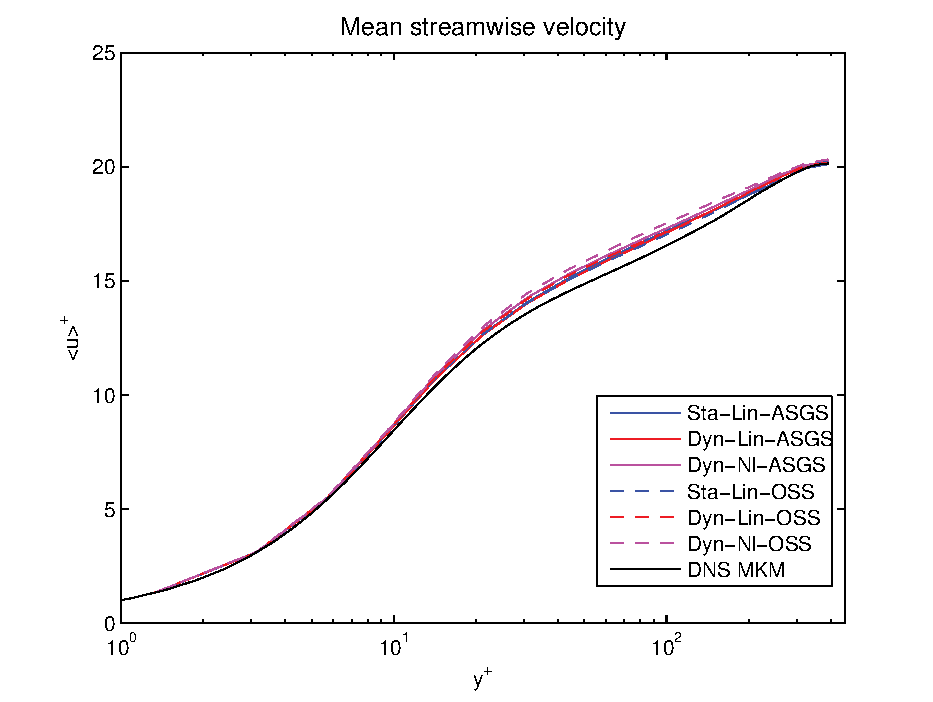
\includegraphics[width=0.49\textwidth]{Figures/Chapter4/CF/umean}}
	\subfigure[Rms stream-wise velocity fluctuation]{\label{fig:Channel_ufluc_32}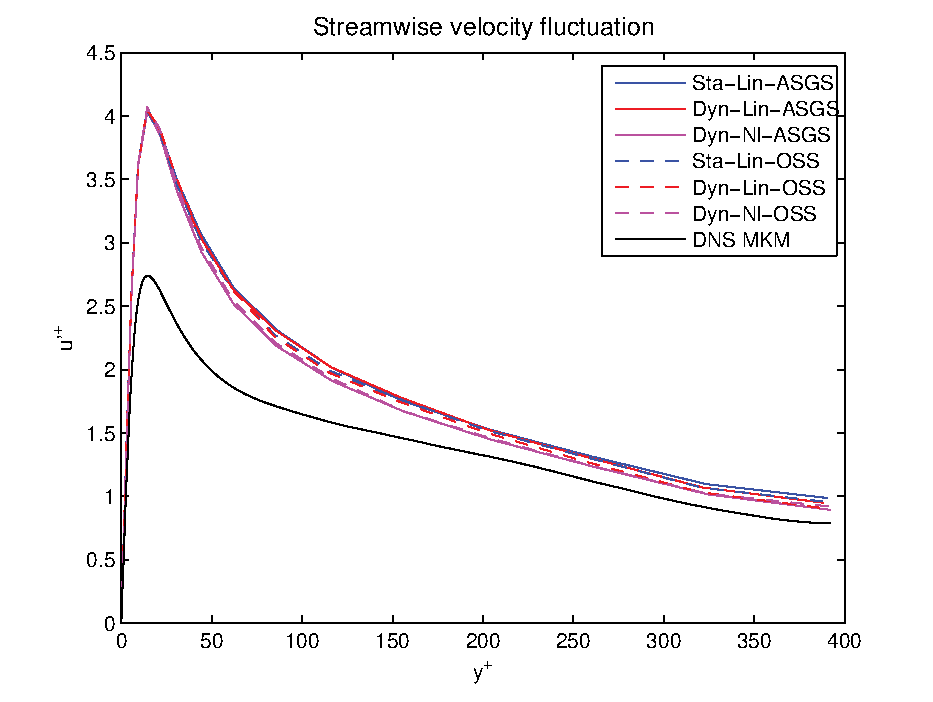
\includegraphics[width=0.49\textwidth]{Figures/Chapter4/CF/ufluc}}\\   
  	\subfigure[Rms wall-normal velocity fluctuation]{\label{fig:Channel_vfluc_32}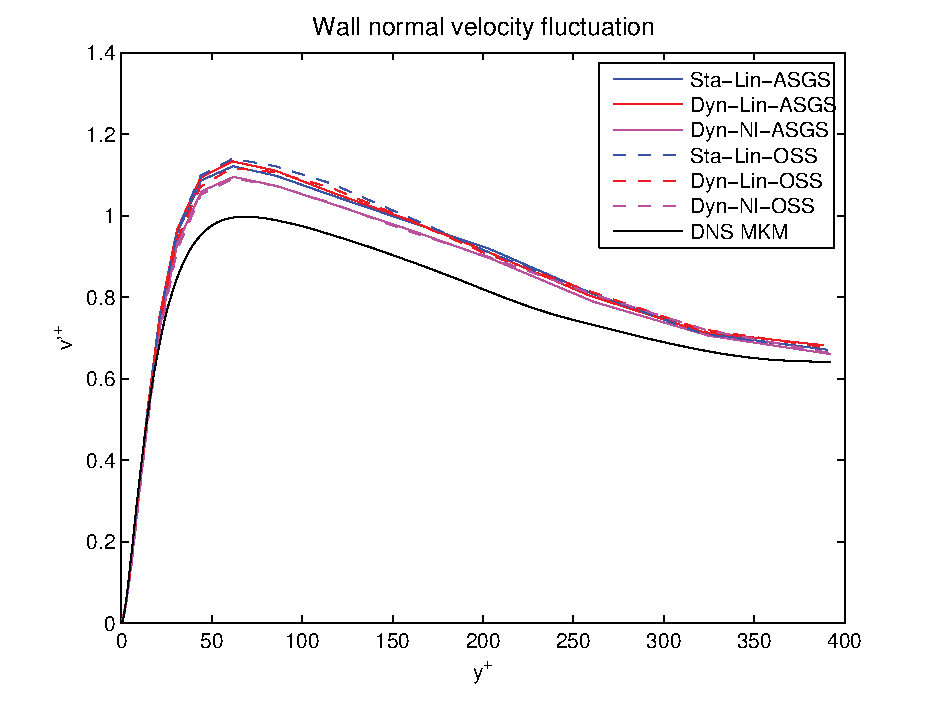
\includegraphics[width=0.49\textwidth]{Figures/Chapter4/CF/vfluc}}
  	\subfigure[Rms span-wise velocity fluctuation]{\label{fig:Channel_wfluc_32}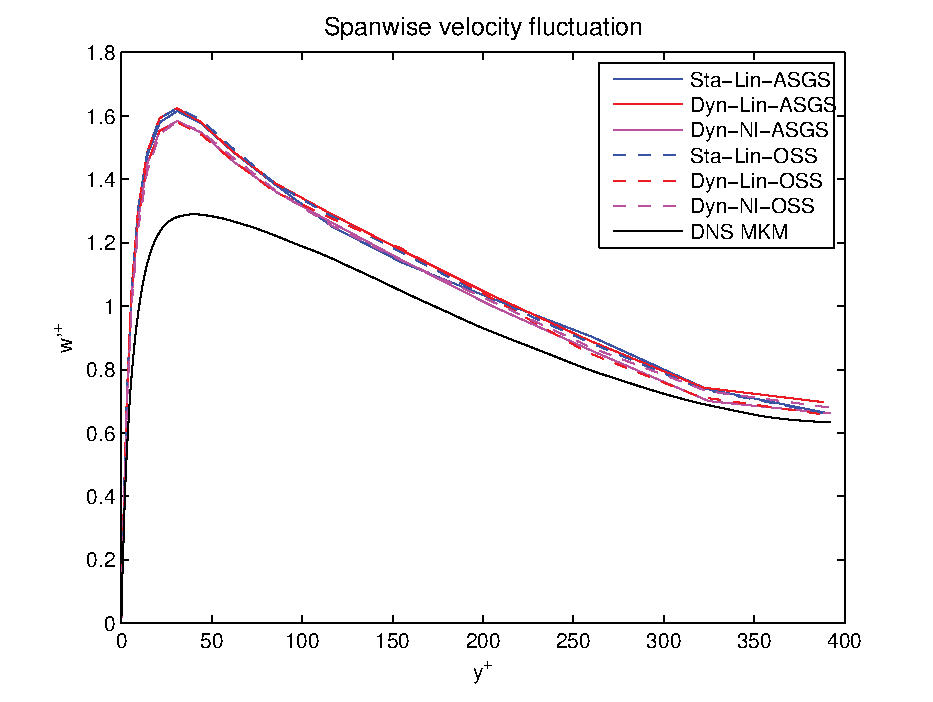
\includegraphics[width=0.49\textwidth]{Figures/Chapter4/CF/wfluc}}
	\caption{Mean stream-wise velocity and rms velocity fluctuations for ${\rm Re}_\tau=395$ case using a $32^3$ $Q$1 mesh.}
	\label{fig:Channel_re395_32}
\end{figure}

\subsubsection{Reynolds shear stress}

Another turbulent quantity widely used in the TCF test is the Reynolds shear stress. At the continuous level the Reynolds shear stress is defined as
\begin{equation}
\label{eq-C4_Rey_shear_cont}
R_{xy}=-\left\langle u'v'\right\rangle+\nu\frac{\partial\left\langle u\right\rangle}{\partial y},
\end{equation}
being $u$ and $v$ the velocity in the streamwise direction and wall-normal direction, respectively,
and the prime denoting the fluctuations, i.e., the variable minus the mean.

It can be seen that for the discrete equation (\ref{eq-C4_NS_discrete}), one can obtain the Reynolds shear stress defined as follows:
\begin{equation}
\label{eq-C4_Rey_shear_disc}
R_{xy}=-\left\langle a_x'a_y'\right\rangle+\nu\frac{\partial\left\langle u_h\right\rangle}{\partial y}=-\underbrace{\left\langle u_h'v_h'\right\rangle}_I-\underbrace{\left\langle u_h'\tilde{v}'\right\rangle-\left\langle \tilde{u}'v_h'\right\rangle-\left\langle \tilde{u}'\tilde{v}'\right\rangle}_{II}+\underbrace{\nu\frac{\partial\left\langle u_h\right\rangle}{\partial y}}_{III}.
\end{equation}
being $a_i$ the $i$-th component of the advection velocity. In (\ref{eq-C4_Rey_shear_disc}) we have used the nonlinear definition of the advection velocity defined in \Eq{C2_a_nl}.

The first term on the second part of  (\ref{eq-C4_Rey_shear_disc}) (term $I$) is the contribution of the resolved scales (FE component) to the cross term $\left\langle a_x'a_y'\right\rangle$. Term $II$ denotes the contribution of the subgrid scales and their interaction with the FE components, that is, the unresolved part of the equation. Finally, term $III$ accounts for the viscous portion of the Reynolds shear stress. Note that the derivatives of the approximated subscales are not computable, since these approximated subscales are discontinuous and have been designed to approximate the effect of the exact subscales on the FE scales element-wise. 

For a fully developed and statistically stable turbulent flow, the Reynolds shear stress along the wall-normal direction has a linear shape  (see \cite{kim_turbulence_1987}). Normalized by the viscous term $III$ value at the wall, the total Reynolds shear stress in terms of $y/	\delta$ should have the following expression: $R_{xy}(y/\delta)=(-y/\delta)$. Fig.~\ref{fig:OSS_dyn_Nl_reystr} depicts the absolute value of the Reynolds shear stress along the upper half channel ($y>0$), with the different terms appearing in (\ref{eq-C4_Rey_shear_disc}) and compared with the DNS in \cite{moser_direct_1999}, for the Dyn-Nl-OSS case with ${\rm Re}_\tau=395$. The computed results are almost identical to the DNS ones. It has to be noted that the computed results are evaluated at the integration points due to the presence of the derivative in the Reynolds shear stress, which using linear FEs is constant at each element. Then, using two integration points per direction for the numerical integration, term $III$ will be constant for those two integration points being in the same element. This behavior is observed in Fig.~\ref{fig:OSS_dyn_Nl_reystr}, where the viscous term is pairwise constant. This last fact also affects the total Reynolds shear stress. Since the resolved term has different values at each element Gauss point, the sum of terms $I$ and $III$ results in an oscillatory shape near the wall, where the viscous term is more relevant. It is also seen that the unresolved term $II$ does not contribute to the Reynolds shear stress, which is a good property of the tested VMS methods. The results for the remaining cases in Table \ref{table:DHIT_cases} are similar to those presented in Fig. \ref{fig:OSS_dyn_Nl_reystr} and have not been reported. 
\begin{figure}[h!]
	\centering	
	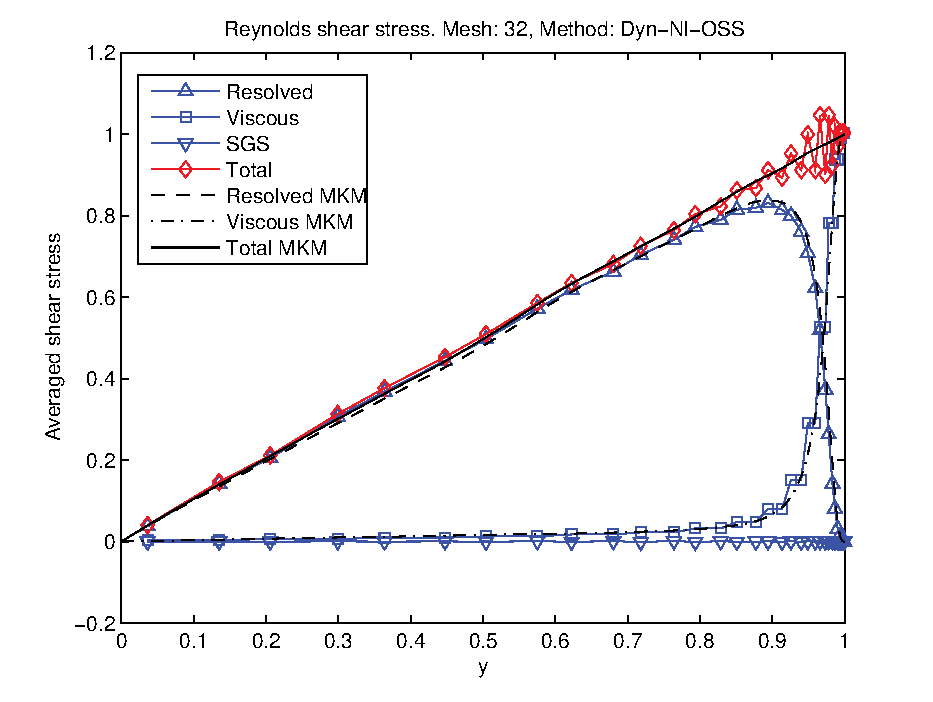
\includegraphics[width=0.5\textwidth]{Figures/Chapter4/CF/reystr_395_Dyn_Nl_OSS}
	\caption{Reynolds stress of the Dyn-Nl-OSS case.}
	\label{fig:OSS_dyn_Nl_reystr}
\end{figure}
% SB: Some change?
%{\color{blue} Esta seccion está perfecta, no tengo que tocar nada. However, si en la turbulencia homogenea calculamos los resultados usando $\u_h$ solamente...porque aca incluimos tambien $\tilde{\u}$?}

\subsection{Sensitivity with respect to the stabilization parameters}
\label{subsec-C4_effect_const}

All the VMS models considered herein depend on the stabilization parameters $\tau_m$ and $\tau_c$, which contain constants $c_1$ and $c_2$ whose value is chosen from numerical experiments. However, we can infer from (\ref{eq-C4_static_energy}) or (\ref{eq-C4_transfer}) how this dependency will be. As mentioned before, the last two terms in (\ref{eq-C4_transfer}) are dissipative and therefore, increasing $\tau_m$ and/or $\tau_c$ we obtain a more dissipative method. From (\ref{eq-C4_tau_m})-(\ref{eq-C4_tau_c}), increasing $\tau_m$ results in a reduction of $\tau_c$. More precisely 
\begin{equation}
\label{eq-C4_tau_c_new}
\tau_c=\nu + \frac{c_2}{c_1}{|\a|}{h}
\end{equation}
from where we see that increasing $c_1$ reduces both $\tau_m$ and $\tau_c$ but increasing $c_2$ reduces $\tau_m$ but increases $\tau_c$. On the other hand, only the fourth term in (\ref{eq-C4_transfer}) is essential to control
$ \tau_{m} \left\| \mathcal{P} \left( \mathbf{a}\cdot \mathbf{\nabla u}_{h}+\mathbf{\nabla }p_{h}\right) \right\|^{2} $ and it is possible to choose $\tau_c=0$. 

The results presented above have been obtained using different settings of the numerical stabilization parameters $\tau_m$ and $\tau_c$. In DHIT and TGV tests, we take the algorithmic constants $c_1=12$ and $c_2=2$ for $\tau_m$ and we set $\tau_c=0$, while for the TCF test we have used $c_1=12$ and $c_2=8$ for $\tau_m$ and also $\tau_c=0$. In this section we analyze the influence of these parameters on the numerical results and justify our choice of the constants for the large eddy simulation of turbulent flows.

We have performed a sensitivity analysis of the VMS schemes with respect to the value of $c_1$ and $c_2$. To see the effect of such algorithmic constants on $\tau_m$ and $\tau_c$ independently, we define a new constant $c_c$ which allows us to redefine (\ref{eq-C4_tau_c_new}) as
\begin{equation}
\label{eq-C4_tau_c_cc_new}
\tau_c=c_c\left(\nu + \frac{c_2}{c_1}{|\a|}{h}\right)
\end{equation}
These experiments have been done for the DHIT test using the Dyn-Nl-OSS case in a $32^3$ $Q$1 mesh and the results are depicted in Fig.~\ref{fig:tau_analysis}. They show important changes in the dissipation the VMS methods introduce when constants are changed. %, as energy dissipation and energy spectra. 
%{\color{blue} 
It is known that the decay rate of kinetic energy in isotropic turbulence is driven by large scales (of the order of the integral scale) (see, e.g., \cite{comte-bellot_simple_1971}). As we have observed, the subgrid model has only influence when a very coarse grid is used.
%} 

In particular, for high Reynolds number problems, the constant $c_1$ does not have so much influence on $\tau_m$, but it does on $\tau_c$. With respect to $c_2$, we observe that it influences the energy dissipation of the method, which is increased when the value of this constant is decreased. When $\tau_c$ is activated ($c_c=1)$, we observe a growth of the energy dissipation when the coefficient $c_2/c_1$ increases. This behavior is what we are expecting since the method becomes more diffusive  when $\tau_c$ is increased due to the last term in (\ref{eq-C4_transfer}).


Concerning the energy spectra, it is also shown in Fig.~\ref{fig:spec_tauc0_t04} and Fig.~\ref{fig:spec_tauc0_t08} that the only constant that influences the result when $\tau_c=0$ is $c_2$. In these figures we can see that when we increase $c_2$ the method is less dissipative, resulting in an inappropriate slope of the energy spectra. We can observe that with $c_2=2$ the decay of the energy behaves correctly, keeping the $k^{-5/3}$ law. For the largest values of $c_2$ the energy at small scales is not properly dissipated. Note that for $c_2=2$ the slope of the energy spectrum is kept almost constant along the time, which does not happen in the other cases. When we activate $\tau_c$ (see Figs. \ref{fig:spec_tauc1_t04} and \ref{fig:spec_tauc1_t08}) we are introducing additional dissipation into the system that eliminates the pile up of the energy spectra for all the cases, but generally results in steeper slopes. Here we also have to note that the energy spectra slope is time dependent for all cases except for $c_2=2$.
%{\color{red} To improve with references and better explanation of the energy spectra correct behavior}
This analysis led us to choose $c_1=12$ and $c_2=2$ for $\tau_m$ and set $\tau_c=0$ for homogeneous turbulence, i.e., DHIT and TGV tests.

%\begin{figure}[h!]
%  \centering
%  \subfigure[Energy with $c_1=12$, $c_2=8$ and $c_c$ variable]{\label{fig:tau_analysis_cc} 
%  \includegraphics[width=0.49\textwidth]{Figures/DHIT/ene_tauc_close}}    
%  \subfigure[Energy with $c_1$ and $c_2$ variable and $c_c=0$]{\label{fig:tau_analysis_c12}
%  \includegraphics[width=0.49\textwidth]{Figures/DHIT/ene_taum_close}}
%  \caption{Comparison of the global energy in the DHIT test for Dyn-Nl-OSS method using a $32^3$ $Q$1 mesh}
%  \label{fig:tau_analysis}
%\end{figure}

% \afterpage{
% \begin{landscape}
\begin{figure}[h!]
\begin{center}
%\begin{tabular}{c@{}c@{}c@{}c}
\begin{tabular}{@{}c@{}c}
%\multirow{2}{*}{\subfigure[Legend]{\label{fig:legend}
%\includegraphics[clip=true,trim=14cm 15cm 16cm 4cm,width=0.2\textwidth]{Figures/DHIT/legend}}} &
%\subfigure[Global energy with $c_c=0$]{\label{fig:ene_tauc0}
%\includegraphics[width=0.42\textwidth]{Figures/DHIT/ene_tauc0}} &
\subfigure[Energy spectra at $t=0.4$ with $c_c=0$]{\label{fig:spec_tauc0_t04}
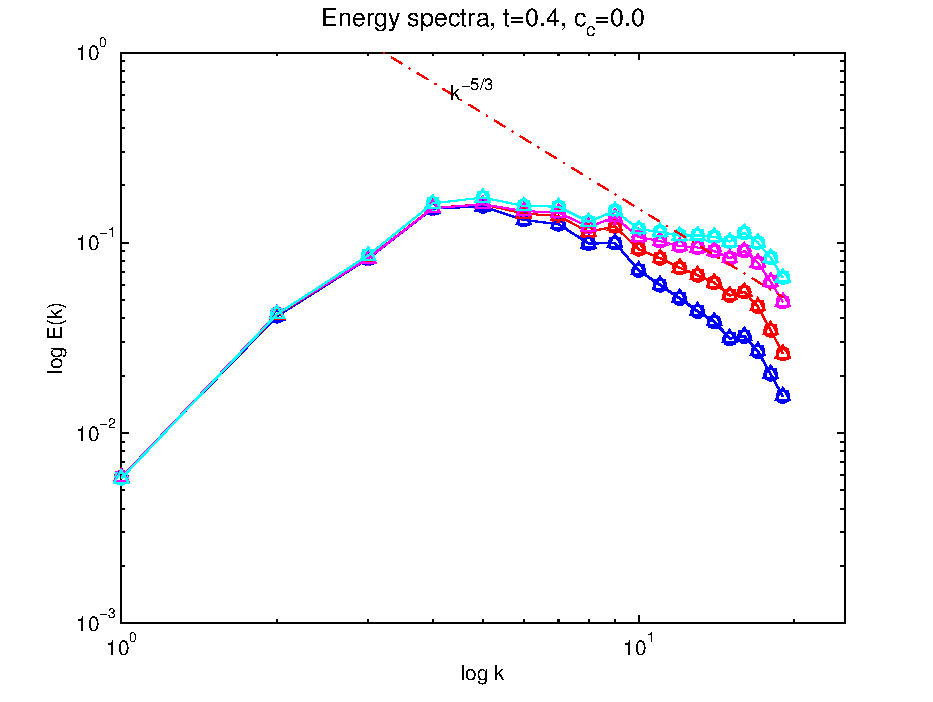
\includegraphics[width=0.48\textwidth]{Figures/Chapter4/DHIT/spec_tauc0_t04}} &
\subfigure[Energy spectra at $t=0.8$ with $c_c=0$]{\label{fig:spec_tauc0_t08}
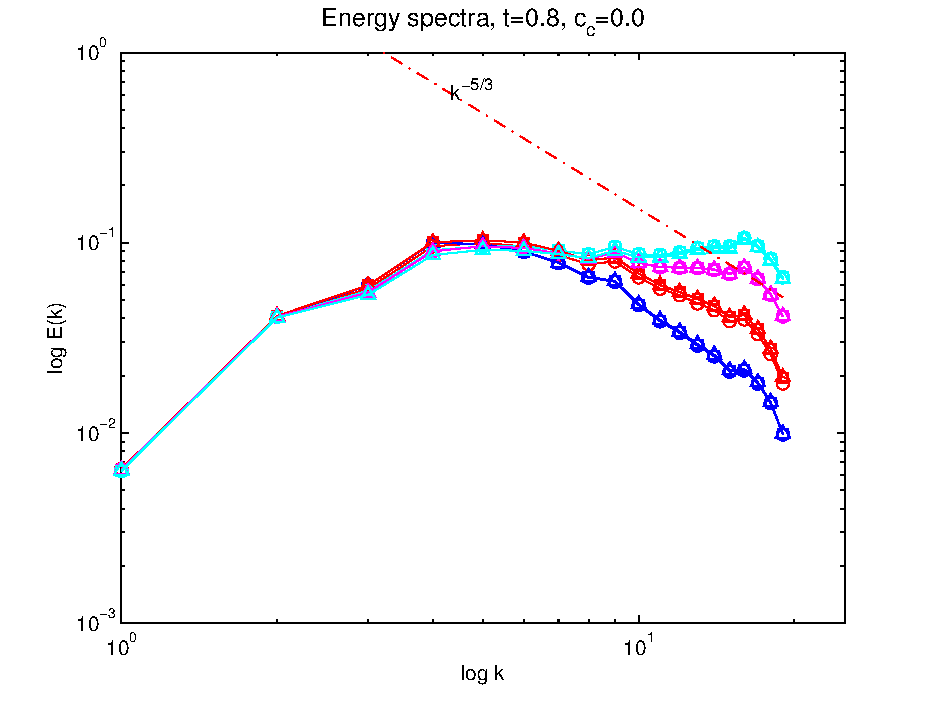
\includegraphics[width=0.48\textwidth]{Figures/Chapter4/DHIT/spec_tauc0_t08}} \\
%\subfigure[Global energy with $c_c=1$]{\label{fig:ene_tauc1}
%\includegraphics[width=0.42\textwidth]{Figures/Chapter4/DHIT/ene_tauc1}} &
\subfigure[Energy spectra at $t=0.4$ with $c_c=1$]{\label{fig:spec_tauc1_t04}
\includegraphics[width=0.48\textwidth]{Figures/Chapter4/DHIT/spec_tauc1_t04}} &
\subfigure[Energy spectra at $t=0.8$ with $c_c=1$]{\label{fig:spec_tauc1_t08}
\includegraphics[width=0.48\textwidth]{Figures/Chapter4/DHIT/spec_tauc1_t08}} \\
\multicolumn{2}{c}{\subfigure[Legend]{\label{fig:legend}
\includegraphics[clip=true,trim=0cm 0cm 0cm 0cm,width=0.6\textwidth]{Figures/Chapter4/DHIT/legend2}}}
\end{tabular}
\end{center}
\caption{Comparison of energy spectra for different $c_1$, $c_2$ and $c_c$ in the DHIT test.}
\label{fig:tau_analysis}
\end{figure}
%\end{landscape}
%}

%{\color{blue}Looking at Figure \ref{fig:tau_analysis}, it seems that the decision to choose $c_1=12$ and $c_2=2$ for $\tau_m$ and set $\tau_c=0$ is the best option among those analysed} {\color{red} for homogeneous turbulence, i.e., DHIT and TGV tests????}.

%{\color{blue}
In order to go in depth on the effect of the algorithmic constants $c_1$ and $c_2$ and the stabilization parameter $\tau_c$ of the incompressibility equation, we compare the results for the TCF problem with a friction Reynolds number ${\rm Re}_\tau=180$ using the same choice made for homogeneous turbulence 
%the setting used until now 
($c_1=12$, $c_2=2$ and $\tau_c=0$) against the setting of the incompressible case in \cite{avila_large_2014} ($c_1=12$, $c_2=2$ and $\tau_c$ as in (\ref{eq-C4_tau_c})) and a less dissipative setting with $c_1=12$, $c_2=8$ and $\tau_c=0$. These tests have been done using the Dyn-Nl-OSS case in a $32^3$ $Q_1$ mesh.
\begin{figure}[h!]
	\centering	
	\subfigure[Mean streamwise velocity]{\label{fig:OSS_taus_umean}\includegraphics[width=0.49\textwidth]{Figures/Chapter4/CF/umean_taus_DOSS}}
  	\subfigure[Rms streamwise velocity fluctuation]{\label{fig:OSS_Matias_ufluc}\includegraphics[width=0.49\textwidth]{Figures/Chapter4/CF/ufluc_taus_DOSS}}\\    
  	\subfigure[Rms wall-normal velocity fluctuation]{\label{fig:OSS_Matias_vfluc}\includegraphics[width=0.49\textwidth]{Figures/Chapter4/CF/vfluc_taus_DOSS}}
 	\subfigure[Rms span-wise velocity fluctuation]{\label{fig:OSS_Matias_wfluc}\includegraphics[width=0.49\textwidth]{Figures/Chapter4/CF/wfluc_taus_DOSS}}
 	\caption{Comparison of mean streamwise velocity and rms velocity fluctuations for ${\rm Re}_\tau=180$ case using a $32^3$ $Q$1 mesh.}
    \label{fig:OSS_taus_fluc}
\end{figure}

In Fig. \ref{fig:OSS_taus_umean} the mean velocity in the streamwise direction is shown. As in the case of homogeneous turbulence, some differences between the three cases can be observed, the choice used in section \ref{subsec-C4_TCF} being the most accurate one. The effect of the algorithmic constant $c_2$ and the stabilization parameter $\tau_c$ in the problem solution can be clearly observed, i.e., the less dissipative choice gives the best results.
%Not only  $\tau_c=0$ but also setting $c_2=8$ (instead of $c_2=2$) give less dissipative results.
Figs. \ref{fig:OSS_Matias_ufluc}, \ref{fig:OSS_Matias_vfluc} and \ref{fig:OSS_Matias_wfluc} depict the rms velocity fluctuations in all directions. The fluctuations in the streamwise direction are better predicted using ($c_1=12$, $c_2=8$ and $\tau_c=0$) but the span-wise and wall-normal directions are not.

\subsection{Behavior in the small time step limit}
\label{subsec-C4_small_time_step}

Small time step instabilities for VMS LES simulations of turbulent flows have been reported in \cite{hsu_improving_2010,gamnitzer_time-dependent_2010}. In these references, the VMS models differ from the ones in this work. Instead of the definition of  $\tau_m$ in (\ref{eq-C4_tau_m}), a time step dependent stabilization parameter $\tau_m$
$$
\tau_m=\left(\frac{1}{\delta t} + \frac{c_1\nu}{h^2}+\frac{c_2|\a|}{h}\right)^{-1},\\
$$
is considered in all cases.\footnote{The parameter $\tau_{m,t}$ for the dynamic subscales model also
scales with $\delta t$, as discussed in Section (\ref{sec-C4_discrete}). {\it However}, this dependence comes from a consistent time integration of the subscale time derivative (see also \cite[Section 3.2]{codina_time_2007}).} The plain introduction of a time step dependency in $\tau_m$ faces serious difficulties:
\begin{itemize}
\item The method becomes unstable in the small time step limit since it converges to the unstable Galerkin formulation.
%\item A similar situation occurs in the Navier-Stokes problem if $\tau_c=0$.
\item If $\tau_c$ is computed from (\ref{eq-C4_tau_c}) (as it is usually done, see, e.g., \cite{bazilevs_variational_2007,hsu_improving_2010,gamnitzer_time-dependent_2010,gravemeier_algebraic_2010}), $\tau_m \sim \delta t$ and $\tau_c \sim \delta t^{-1}$ in the small time step limit. If this approach is followed , the essential numerical dissipation given by the fifth term in (\ref{eq-C4_static_energy}) is reduced as $\delta t \to 0$, whereas the numerical dissipation introduced by the last term in the left hand side (a incompressibility penalty term) of (\ref{eq-C4_static_energy}) is increased. It has a compensating effect in practice, but the penalty term does not properly act as a turbulence model. % , as shown in the previous section.
\end{itemize}
%The behavior of the VMS models considered herein in the small time step limit is evaluated numerically in Section \ref{sec-C4_TCF}.

Let us perform a test to study the small time step behavior of the VMS methods presented in Section \ref{sec-C4_prob_statement}, using the skew-symmetric \textit{type 1} form of the convective term, as in previous numerical experiments. We also include a combination we do not advocate here, static subscales and nonlinear splitting, an approach followed in \cite{Calo_2004,bazilevs_variational_2007,hsu_improving_2010,gamnitzer_time-dependent_2010,gravemeier_algebraic_2010}. %The properties of the different methods in this respect have been discussed in Section \ref{subsec-C4_small_time_step}. 
The behavior of all the methods for the TCF test with $\delta t=0.002$ is summarized in Table \ref{table:small_time_step_T}, where YES means that the simulation was successful, NO means that the simulation diverged and $\delta t\downarrow$ means that the simulation was successful only when the adaptive time step strategy described in Section \ref{subsubsec-C4_DHIT_setting} was used.

%It is worth to point out that all these results have been obtained using the skew-symmetric \textit{type 1} form of the convective term, which exactly conserves energy. %Either a conservative or non conservative form is usually employed mentioned references and none of this forms conserve energy. As we have shown in Section \ref{subsubsec-C4_ene_cons_DHIT} for the skew-symmetric \textit{type 2}, they could be productive. 
It is important to note that the static and nonlinear ASGS formulation used in \cite{bazilevs_variational_2007,hsu_improving_2010,gamnitzer_time-dependent_2010,gravemeier_algebraic_2010} with the convective term \textit{type 2} becomes unstable after some time, as also reported in these works, even for the time step size defined in section \ref{subsubsec-C4_TCF_setting}. However, using the the skew-symmetric \textit{type 1} form of the convective term, which exactly conserves energy, the simulation ended successfully for the time step defined in section \ref{subsubsec-C4_TCF_setting}, but failed to converge with the small one. This result is a numerical evidence of the fact that the use of convective terms without the skew-symmetric property produce energy (see also Section \ref{subsubsec-C4_Total_ene_DHIT}) that can make simulations unstable. Further, \emph{these results evidence once again that it is a good choice to stick to provably unconditionally stable formulations, i.e., the dynamic formulations and/or orthogonal subscales formulations with a skew-symmetric convective term}. %{\color{blue} 
Similar results have been reported in the finite difference context in \cite{verstappen_symmetry-preserving_2003}, where it is shown that stable simulations of the TCF can be performed using an energy-preserving skew-symmetric formulation.
%}

\begin{table}[h!]
%\label{tab:small_dt}
%\footnotesize
\centering
\begin{tabular}{ccccccccc}
\toprule
Method&\multicolumn{4}{c}{ASGS}&\multicolumn{4}{c}{OSS}\\
\midrule
Tracking&\multicolumn{2}{c}{Static}&\multicolumn{2}{c}{Dynamic}&\multicolumn{2}{c}{Static}&\multicolumn{2}{c}{Dynamic}\\
\midrule
Advection&Linear&Nonlinear&Linear&Nonlinear&Linear&Nonlinear&Linear&Nonlinear\\
\midrule
Converged&Yes&No&Yes&Yes&$\delta t\downarrow$&$\delta t\downarrow$&Yes&Yes\\
\bottomrule
\end{tabular}
\caption{Small time step convergence analysis.}
\label{table:small_time_step_T}
\end{table}

%Furthermore, keeping aside the stability of the methods, 
To the best of our knowledge, the stability (or instability) of dynamic ASGS methods has not been proved. In our numerical experiments the static and dynamic linear versions fail to converge in some problems (e.g DHIT) but we have not found these problems with the Dyn-Nl-ASGS method. Nevertheless, we have found an important increase in the computational cost when the time step is reduced. 
%the time step size also has an effect on the computational cost. 
%In particular, the number of solver iterations for ASGS methods increase when the time step is reduced. 
This behavior is explained in Fig. \ref{fig:1st_step_comp_cost}, where the number of solver iterations at the first time step is plotted against the time step size for the dynamic and nonlinear cases of ASGS and OSS methods, with $32^3$ and $64^3$ $Q_1$ mesh, for the DHIT test case. \emph{The number of required solver iterations (and as a result the condition number of the system matrix) blows up exponentially for the ASGS method as we reduce the time step size, whereas it remains constant for the OSS method.} This important observation explains the computational cost trends observed in the previous section.
\begin{figure}[h!]
	\centering	
	\includegraphics[width=0.5\textwidth]{Figures/Chapter4/DHIT/1st_step_comp_cost}
	\caption{Solver iterations at the first time step for DHIT test.}
	\label{fig:1st_step_comp_cost}
\end{figure}

%Finally, it is clearly seen in Fig. \ref{fig:1st_step_comp_cost} the exponential increase of solver iterations for the ASGS methods when the time step tends to zero, independently of the mesh size. This performance denotes the \emph{ill conditioning of the ASGS system matrix with respecto to the time step size}. On the other hand, \emph{the number of solver iterations remains constant for the OSS method}, regardless of the time step size.

%%\subsubsection{Numerical dissipation}
%%
%%\begin{figure}[h!]
%%	\centering	
%%	\includegraphics[width=0.5\textwidth]{Figures/CF/numdis_395_Dyn_Nl_OSS}
%%	\caption{Numerical dissipation of the Dyn-Nl-OSS case}
%%	\label{fig:OSS_dyn_Nl_numdis}
%%\end{figure}
%
\section{Conclusions}
\label{sec-C4_conclusions}

In this paper we have assessed the performance of the numerical formulations previously developed in our group \cite{codina_stabilized_2002,codina_time_2007,Codina-chap-2011,principe_dissipative_2010} for turbulent incompressible flow problems. 

The methods proposed are different to those whose testing in turbulent regimes has been published before, the closest ones being those reported in \cite{bazilevs_variational_2007,gamnitzer_time-dependent_2010}. First, we consider orthogonal subscales formulations. Further, in \cite{bazilevs_variational_2007} the ASGS method with quasi-static subscales is used (in the isogeometrical analysis context) but the time step dependency is included in the stabilization parameter (with the inconsistencies and problems discussed in section \ref{subsec-C4_small_time_step}) and the nonlinear scale splitting is applied in the FE equation only (not in the subscale equation). Time dependent subscales are used in \cite{gamnitzer_time-dependent_2010}, but the authors consider a linear scale splitting. Furthermore, in both works $\tau_c \neq 0$. 

First, we have discussed some theoretical aspects, such as the dissipative structure of the methods and the way energy is conserved, which we have numerically verified. Related to this point, we analyze the effect of using different skew-symmetric forms of the convective term, and its impact on energy conservation; if a skew symmetric form is not used, negative energy dissipation can be introduced to the scheme, which may be a source of instability. 

However, the most important conclusions come from the different problems that we have solved numerically. Overall, OSS and ASGS yield similar results, all displaying the features of turbulent flows, reproducing appropriately global outputs such as energy spectra. The methods are stable and converge to reference solutions, both when the mesh is refined and when the polynomial order is increased. 

On the other hand, we have thoroughly analyzed the effect of the algorithmic constants for isotropic turbulence and wall-bounded turbulent flows, and chosen them based on this sensitivity analysis. An important observation in this line is the fact that all the methods considered in this work are certainly sensitive to the algorithmic constants and they have to be properly chosen in order to simulate turbulent flows on coarse meshes. In fact, the differences in the numerical results are much more influenced by the algorithmic constants than by the choice of the VMS formulation itself.  This strong influence seems to be a characteristic feature of turbulence, since in our experience it is not so important in laminar flows. VMS methods is something that needs further research.

Further, we have analyzed the effect of small time steps when the stabilization parameters depend on them.


Apart from the quality of the results, the OSS method with dynamic subscales is convenient in terms of numerical performance. It requires more nonlinear iterations than ASGS, but less iterations of the linear solver, altogether leading to lower computational cost. In both formulations, ASGS and OSS, the use of dynamic subscales has been found to be crucial for nonlinear convergence. In fact, in some cases quasi-static subscales failed to converge. We have explained these facts by plotting the number of solver iterations required to converge as we reduce the time step size, for a fixed mesh in space. The number of iterations (and as a result the condition number of the system matrix) blows up exponentially for ASGS whereas it remains bounded for OSS.